\documentclass[a4paper]{article}
\usepackage[utf8]{inputenc} 
\usepackage[spanish]{babel} 
\usepackage{caratula}

% Comandos para simbolos matematicos.
\usepackage{enumitem}
\usepackage{amsmath}
\usepackage{amssymb}
\usepackage{tabularx}

% Uno de estos imports rompe la carátula
%\usepackage{amsfonts,epsfig,epstopdf,titling,url,array}

% Configuración para usar tikz
\usepackage{tikz}
\usetikzlibrary{positioning,arrows.meta, shapes.geometric}

% Estilos para dibujar grafos
\tikzset{arco/.style={line width=0.2mm, -latex}}
\tikzset{arista/.style={line width=0.2mm}}
\tikzset{blabel/.style={midway,below,draw=none,fill=none}}
\tikzset{alabel/.style={midway,above,draw=none,fill=none}}
\tikzset{rlabel/.style={midway,right,draw=none,fill=none}}
\tikzset{llabel/.style={midway,left, draw=none,fill=none}}

% Colores
\definecolor{pastelgreen}{RGB}{145,210,144} % RGB format
\definecolor{pastelblue}{RGB}{111,183,214}
\definecolor{pastelred}{HTML}{FF6961}       % Hexadecimal format

% Comandos para referencias
\usepackage{natbib}

% Comandos para Figuras, Graficos, Tikz etc.
\usepackage{tikz}
\usepackage{epsfig}
\usepackage{pgfplots}
\usepackage{graphicx}
\usepackage{caption}
\usepackage{prettyref,cleveref}
\DeclareCaptionFont{white}{\color{white}}
\DeclareCaptionFormat{listing}{\colorbox[cmyk]{0.43, 0.35, 0.35,0.01}{\parbox{\textwidth}{\hspace{15pt}#1#2#3}}}

\usepackage{subcaption}
\usepackage{svg}
\setsvg{inkscapeexe=inkscape inscapeopt=-z -D}

% Comandos para algoritmos.
\usepackage[noend]{algpseudocode}
\usepackage{algorithm}
\algnewcommand{\IfThenElse}[3]{% \IfThenElse{<if>}{<then>}{<else>}
\State \algorithmicif\ #1\ \algorithmicthen\ #2\ \algorithmicelse\ #3}
\algnewcommand{\IfThen}[2]{% \IfThenElse{<if>}{<then>}
  \State \algorithmicif\ #1\ \algorithmicthen\ #2}
\pgfplotsset{compat=1.16}

% FORMATO

% Formato de párrafos
\setlength{\parskip}{0.5em}

% Formato de páginas
\usepackage{fancyhdr}
\pagestyle{fancy}

\renewcommand{\sectionmark}[1]{\markright{\thesection\ - #1}}

\fancyhf{}

\fancyhead[LO]{Sección \rightmark} % \thesection\ 
\fancyfoot[LO]{\small{Cerdeira, Gianatiempo, Panichelli, Schuster}}
\fancyfoot[RO]{\thepage}
\renewcommand{\headrulewidth}{0.5pt}
\renewcommand{\footrulewidth}{0.5pt}

\setlength{\hoffset}{-0.8in}
\setlength{\textwidth}{16cm}
\setlength{\headsep}{0.5cm}
\setlength{\textheight}{25cm}
\setlength{\voffset}{-0.7in}
\setlength{\headwidth}{\textwidth}
\setlength{\headheight}{13.1pt}

\renewcommand{\baselinestretch}{1.1}  % line spacing

% ******************************************************** %

\begin{document}

\thispagestyle{empty}
\materia{Algoritmos y Estructura de Datos III}
\submateria{Segundo Cuatrimestre de 2020}
\titulo{Trabajo Práctico II}
\subtitulo{\textit{PCMI}}
\grupo{Grupo 15}

\integrante{Cerdeira, Elías Nahuel}{692/12}{eliascerdeira@gmail.com}
\integrante{Gianatiempo, Octavio}{280/10}{ogianatiempo@gmail.com}
\integrante{Panichelli, Manuel}{72/18}{panicmanu@gmail.com}
\integrante{Schuster, Martín}{208/18}{m.a.schuster98@gmail.com}

\maketitle

\newpage

\thispagestyle{empty}
\vfill

% Temas a hablar por seccion
% 
% Abstract
%   - lo de siempre
% 
% Introducción
%  - [DONE] describir el problema de PCMI dando ejs y sols.
%  - [WIP]  situaciones de la vida real
% 
% Desarrollo
%   - intro teorica de tabu search
%   - Para cada algoritmo (W, WP, TSC-E/C TSS-E/C)
%       - Explicar el algoritmo y dar complejidad
%       - Describir instancias para las cuales no de sols optimas.
%       - Indicar que tan mala puede ser una solucion obtenida respecto de la optima ???
%       mas una cuestion intuitiva, entendiendo como anda darnos cuenta en que instancias o flia de instancias podria andar mal
% 
% Experimentacion
%   - exp 1: comparar golosos
%   - exp 2: optimizar meta-parametros
%       - ver como son las instancias que tomamos
%   - exp 3: probar con instancias nuevas
%
% Trabajo futuro
%   - Explorar vecindades menos restrictivas.
%   - ver las diferencias más finas (w vs wp y E vs C) con un conjunto de instancias más grande. Es más probable que las diferencias en el ranking entre entrenamiento y testeo se deban a particularidades de las instancias que quedaron en cada caso. Por eso podemos distinguir bien entre cambios con alto impacto i.e swap vs change pero se introduce ruido en el ranking para diferencias finas.

\thispagestyle{empty}
\vspace{3cm}
\tableofcontents
\newpage

\clearpage
\setcounter{page}{1}

\section{Introducción}

En la vida cotidiana es común tener situaciones donde se deseen asignar, disponer o distribuir elementos según algunas restricciones y/o preferencias. Algunos problemas complejos pueden resolverse con algoritmos de optimización combinatoria. Generalmente, estos algoritmos resuelven instancias de problemas que se consideran difíciles de resolver, explorando el espacio de soluciones (usualmente grande) utilizando algunas heurísticas. Estos algoritmos, además, lo logran reduciendo el tamaño efectivo del espacio ya que exploran el espacio de búsqueda eficientemente.

Un problema conocido de optimización combinatoria es el problema de \textit{coloreo mínimo}, donde se explora el espacio de soluciones válidas (coloreos) y se selecciona aquel que utilice el menor número de colores. En este trabajo, se estudiará un problema alternativo, en el que se desea encontrar un coloreo factible para el grafo $G$ buscando maximizar un función $I$ (impacto) de acuerdo a las relaciones establecidas por otro grafo $H$ que presenta los mismos vértices pero no necesariamente la misma distribución de aristas.

Formalmente, dados dos grafos $G=(V,X_G)$ y $H=(V,X_H)$ definidos sobre el mismo conjunto de vértices $V$ y dado un conjunto de $C$ de colores, se define el impacto $I(c)$ sobre $H$ de un coloreo $c:V\rightarrow C$ de $G$ como el número de aristas $e=(i,j)\in X_H$ tales que $c(i) = c(j)$. Se define entonces el Problema de Coloreo Máximo Impacto (PCMI) como un problema de optimización combinatoria donde se busca maximizar el valor de impacto ($I(c)$) obtenido. Para simplificar, se considera \textit{solución factible} a todo coloreo válido de $G$. Cada coloreo se representa como un arreglo de colores de longitud $n$ donde la posición $i$-ésima corresponde al color del vértice $i$.

A continuación se exhibe un ejemplo con su correspondiente respuesta esperada.

\begin{itemize}
    \item $n=5$ con los grafos $G$ y $H$ representados en la \cref{fig:example-graph}. Las soluciones factibles son todos los coloreos válidos de $G$, como pueden ser [\textit{rojo, verde, amarillo, azul, violeta}] o [\textit{rojo, rojo, azul, azul, rojo}]. El primero corresponde a un coloreo trivial, asignar colores distintos a cada vértice, y presenta un impacto de $0$ debido a que ningún par de vértices comparte colores. El segundo, es el coloreo óptimo ya que todas las aristas de H que no están en G, es decir todas las que podrían contribuir al impacto sin invalidar el coloreo si unieran dos vértices del mismo color, efectivamente unen dos vértices del mismo color.
\end{itemize}

\begin{figure}[H]
    \centering
    \begin{subfigure}[H]{0.45\textwidth}
        \centering
        \begin{tikzpicture}[scale = 1, every node/.style={draw,circle}] 
            \node[] (1) at (0,0) {1};
            \node[below right= 4mm  and 7mm   of 1] (2) {2};
            \node[below right= 16mm and 2.5mm of 1] (3) {3};
            \node[below left=  16mm and 2.5mm of 1] (4) {4};
            \node[below left=  4mm  and 7mm   of 1] (5) {5};
            
            \draw[arista] (1) to (3);
            \draw[arista] (1) to (4);
            \draw[arista] (2) to (4);
            \draw[arista] (2) to (3);
        \end{tikzpicture} 
        \caption{Grafo G}
        \label{fig:graphG}
    \end{subfigure}
    \begin{subfigure}[H]{0.45\textwidth}
        \centering
        \begin{tikzpicture}[scale = 1,every node/.style={draw,circle}] 
            \node[] (1) at (0,0) {1};
            \node[below right= 4mm  and 7mm   of 1] (2) {2};
            \node[below right= 16mm and 2.5mm of 1] (3) {3};
            \node[below left=  16mm and 2.5mm of 1] (4) {4};
            \node[below left=  4mm  and 7mm   of 1] (5) {5};
            
            \draw[arista] (1) to (2);
            \draw[arista] (1) to (5);
            \draw[arista] (2) to (5);
            \draw[arista] (3) to (4);
            \draw[arista] (1) to (4);
            \draw[arista] (1) to (3);
            \draw[arista] (2) to (3);
        \end{tikzpicture}
        \caption{Grafo H}
        \label{fig:graphH}
    \end{subfigure}
    \caption{Instancia de ejemplo para el problema de PCMI. El grafo $G$ se utiliza para verificar que el coloreo sea válido, establece restricciones entre nodos, mientras que el grafo $H$ establece las relaciones de impacto.}
    \label{fig:example-graph}
\end{figure}

Algunas situaciones de la vida cotidiana donde se puede encontrar un problema de PCMI podría ser el caso de distribución de invitados en las distintas mesas en un casamiento, cumpleaños o demás fiestas. Cada invitado se representa con un nodo $v\in V$. Luego, como estamos modelando personas reales, existirán enemistades, peleas o cualquier tipo de restricción que impida o sugiera que no es correcto sentar a dos personas en la misma mesa. Estas restricciones se representarán como una arista en el grafo $G$. Luego, tendremos gente que se desee agrupar preferencialmente por algún criterio, como pueden ser parejas, amigos, familiares directos o grupos etarios. Estas relaciones deseables, pero no restrictivas, se modelan como una arista en el grafo $H$. Luego, las distintas mesas (que pueden considerarse de tamaño infinito para simplificar el problema) se pueden representar a través de los colores. Así, es fácil ver que se puede utilizar una solución al problema de PCMI para encontrar una asignación óptima para las personas en las distintas mesas, dado que el coloreo obtenido permite evitar juntar gente que no quiere reunirse y maximiza la cantidad de personas que se quieren poner juntas.

El objetivo de este trabajo es implementar una solución para PCMI utilizando 3 heurísticas golosas constructivas y 2 metaheurísticas y evaluar la efectividad de cada una para distintas instancias. En primer lugar se utiliza el algoritmo de \textit{heurística secuencial de coloreo con orden largest first} (S-LF) que consiste en colorear secuencialmente los vértices del grafo $G$ comenzando por alguno de grado mayor ($\triangle_G(v)$) y asignando el menor número de color posible. Para el algoritmo de \textit{Wyrnística diferencial} (W) se genera un conjunto de aristas $W$ tales que $e \in W \iff e \in X_H \wedge e \not\in X_G$. Luego, para cada arista en $W$, se colorean sus extremos del mismo color. En caso de que uno de los dos esté ya coloreado, ignora ambos vértices y, al terminar, asigna un color distinto a cada vértice no coloreado. Finalmente, la heurística \textit{Wyrnística power} (WP) consiste en realizar el mismo procedimiento anteriormente descrito, excepto que al intentar colorear el par $(v, w) \in W$, si $w$ ya está coloreado, en vez de saltearlo intenta colorear a $v$ del mismo color, siempre y cuando sea válido.

Para el caso de las metaheurísticas, se utilizan para construir una solución inicial todas las heurísticas golosas descritas anteriormente. Por un lado, para el algoritmo \textit{Tabu Search con Swap} (TSS) se explora la vecindad de una solución intermedia intercambiando el color de dos vértices del grafo, mientras que para el algoritmo \textit{Tabu Search con Change} (TSC), se cambia el color de un vértice por algún color válido presente en el coloreo observado. En ambos casos, se utiliza una memoria o \textit{lista tabú} para almacenar soluciones intermedias ya recorridas. En un caso, se almacena de forma \textit{estructural} (E), definiendo qué vértices se intercambiaron o qué color se le asignó al vértice cambiado. En otro, se almacena directamente el \textit{coloreo} (C) completo de la solución revisada.

En la sección de metodología se introducen y explican los algoritmos y las diferencias entre las distintas técnicas junto con las respectivas demostraciones de correctitud y complejidad. Luego, se exponen los experimentos realizados con sus resultados y la respectiva discusión. Por último, se detallan las conclusiones finales del trabajo.

\section{Metodología}\label{metodologia}

Dado que PCMI pertenece a la categoría de problemas $\mathcal{NP}$-hard, en este trabajo se busca dar soluciones de la mejor calidad posible, pero no las óptimas. A continuación se presentan los distintos métodos utilizados para desarrollar algoritmos que lo resuelvan.

\section{Heurísticas constructivas golosas}

Las \textbf{heurísticas constructivas} son métodos que construyen iterativamente una solución factible para una instancia de un problema dado. Se suelen utilizar procedimientos golosos, que si bien no garantizan que las soluciones sean óptimas, retornan soluciones de una calidad aceptable por un costo computacional comparativamente menor. En este trabajo se implementa una heurística existente para el problema de coloreo \textit{(Secuencial - Largest First)} y se definen dos nuevas específicas para PCMI (\textit{Wyrnística Diferencial y Wyrna Power}).

\subsection{Secuencial - Largest First (S-LF)}

La heurística \textbf{secuencial} consiste en recorrer los vértices de forma secuencial y colorear a cada uno con el mínimo posible. La implementación \textbf{Secuencial - Largest First (LF)} los recorre en forma descendiente según su grado, lo cuál hace que genere coloreos más cercanos al óptimo. Es la heurística más natural para colorear los vértices de un grafo y su correctitud es trivial. Es fácil verificar que no genera siempre el coloreo óptimo, lo cual no resulta importante para PCMI dado que sólo interesa optimizar el impacto. En la \cref{fig:slf_coloreo} se presenta el coloreo obtenido con esta heurística.

El Algoritmo~\ref{alg:alg_secuencial} muestra una implementación posible. Es importante notar que es un algoritmo que solo toma en cuenta el grafo $G$ y no considera el impacto que genera. Sin embargo, resulta intuitivo que a menor cantidad de colores, mayor es la probabilidad de que haya un impacto alto.

\begin{algorithm}[H]
    \begin{algorithmic}[1]
        \State{\textbf{Entrada:} los grafos $G$ y $H$ en representación de listas de adyacencias}
        \State{\textbf{Salida:} coloreo de $G$ e impacto}
        \State
        \Function{$secuencialLF$}{$G$, $H$}:
            \State{$vertices \leftarrow \forall v \in G$ pares de $(d_G(v), v)$} \Comment{$O(n)$}
            \State{$sort(vertices)$}\Comment{$O(n\times log(n))$}
            
            \State{$coloreo \leftarrow array_n[undefined$]} \Comment{$O(n)$}
            
            \For{$(g,v)$ \textbf{in} $vertices$}: \Comment{$O(n^2)$}
                \For{$color~c$ \textbf{in} $1..n \wedge coloreo[v]~is~undefined$}:
                     \If{$\nexists\ u \in N_G(v) \mid coloreo[u] = c$} \Comment{$O(n)$}
                            \State{$coloreo[v] = c$}
                        \EndIf
                \EndFor
            \EndFor
    
            \State{\textbf{return} $coloreo$, $impacto(H,coloreo)$} \Comment{$O(m_H)$}
        \EndFunction
        \State{}
        \State{\textbf{Complejidad:} $O(n^2 + n\times log(n)+n + m_H) = O(n^2)$}
    \end{algorithmic}
    \caption{Algoritmo de \textit{Secuencial con ordenamiento Largest First} para PCMI.}
    \label{alg:alg_secuencial}
\end{algorithm}

\begin{figure}[H]
    \centering
    \begin{subfigure}[H]{0.45\textwidth}
        \centering
        \begin{tikzpicture}[scale = 1, every node/.style={draw,circle}] 
            \node[fill=pastelgreen] (1) at (0,0) {1};
            \node[fill=pastelgreen, below right= 4mm  and 7mm   of 1] (2) {2};
            \node[fill=pastelblue,  below right= 16mm and 2.5mm of 1] (3) {3};
            \node[fill=pastelblue,  below left=  16mm and 2.5mm of 1] (4) {4};
            \node[fill=pastelgreen, below left=  4mm  and 7mm   of 1] (5) {5};
            
            \draw[arista] (1) to (3);
            \draw[arista] (1) to (4);
            \draw[arista] (2) to (4);
            \draw[arista] (2) to (3);
        \end{tikzpicture} 
        \caption{Grafo G}
    \end{subfigure}
    \begin{subfigure}[H]{0.45\textwidth}
        \centering
        \begin{tikzpicture}[scale = 1,every node/.style={draw,circle}] 
            \node[fill=pastelgreen] (1) at (0,0) {1};
            \node[fill=pastelgreen, below right= 4mm  and 7mm   of 1] (2) {2};
            \node[fill=pastelblue,  below right= 16mm and 2.5mm of 1] (3) {3};
            \node[fill=pastelblue,  below left=  16mm and 2.5mm of 1] (4) {4};
            \node[fill=pastelgreen, below left=  4mm  and 7mm   of 1] (5) {5};
            
            \draw[arista] (1) to (2);
            \draw[arista] (1) to (5);
            \draw[arista] (2) to (5);
            \draw[arista] (3) to (4);
            \draw[arista] (1) to (4);
            \draw[arista] (1) to (3);
            \draw[arista] (2) to (3);
        \end{tikzpicture}
        \caption{Grafo H}
    \end{subfigure}
    \caption{Instancia de ejemplo para el problema de PCMI. Se presenta el coloreo esperado obtenido al correr el algoritmo presentado para la heurística S-LF.}
    \label{fig:slf_coloreo}
\end{figure}

Dado que esta heurística colorea a cada vértice con el mínimo que pueda asignarle sin tener en cuenta $H$, dados 3 vértices, $u, v, w$ tales que $(v, w) \in X_H, (u, v) \in X_G$ y $d_G(u) > d_G(v) > d_G(w)$, se colorea primero a $u$, luego a $v$ de un color diferente a $u$ y finalmente a $w$ del mismo color de $u$. Como resultado, $u$ tiene un color diferente al de $v$, reduciendo así el impacto.

Esto puede extenderse a clases de instancias, donde dados $u$ y $v$, $u$ es universal en $G - v$ (pero aislado en $H$) y $v$ universal en $H - u$ (pero aislado en $G$). $u$ no es adyacente a $v$. Se colorea primero a $v$ por ser el de grado máximo en $G$ del color $1$, luego a todos menos $v$ del color $2$, y finalmente a $v$ del color 1, llevando a un impacto 0 sin importar que tan grande sea el grafo, cuando en realidad el impacto máximo es $n - 1$. 

\begin{figure}[H]
    \centering
    \begin{subfigure}[H]{0.45\textwidth}
        \centering
        \begin{tikzpicture}[scale = 1, every node/.style={draw,circle}] 
            \node[]  (1) at (0,0) {$v$};
            \node[below right= 8mm  and 9.5mm of 1] (2) {2};
            \node[below right= 21mm and 4mm   of 1] (3) {3};
            \node[below left=  21mm and 4mm   of 1] (4) {4};
            \node[below left=  8mm  and 9.5mm of 1] (5) {5};
            \node[below = 7mm of 1] (6) {$u$};

            %\draw[arista] (6) to (1);
            \draw[arista] (6) to (2);
            \draw[arista] (6) to (3);
            \draw[arista] (6) to (4);
            \draw[arista] (6) to (5);
        \end{tikzpicture} 
        \caption{Grafo G}
    \end{subfigure}
    \begin{subfigure}[H]{0.45\textwidth}
        \centering
        \begin{tikzpicture}[scale = 1,every node/.style={draw,circle}] 
            \node[]  (1) at (0,0) {$v$};
            \node[below right= 8mm  and 9.5mm of 1] (2) {2};
            \node[below right= 21mm and 4mm   of 1] (3) {3};
            \node[below left=  21mm and 4mm   of 1] (4) {4};
            \node[below left=  8mm  and 9.5mm of 1] (5) {5};
            \node[below = 7mm of 1] (6) {$u$};

            \draw[arista, color=pastelblue] (1) to [bend right=30] (5);
            \draw[arista, color=pastelblue] (1) to [bend left= 30] (2);
            \draw[arista, color=pastelblue] (1) to [bend left= 30] (3);
            \draw[arista, color=pastelblue] (1) to [bend right=30] (4);
        \end{tikzpicture}
        \caption{Grafo H}
    \end{subfigure}
    \vspace{}
    \begin{subfigure}[H]{0.45\textwidth}
        \centering
        \begin{tikzpicture}[scale = 1, every node/.style={draw,circle}] 
            \node[fill=pastelgreen] (1) at (0,0) {$v$};
            \node[fill=pastelblue, below right= 8mm  and 9.5mm of 1] (2) {2};
            \node[fill=pastelblue, below right= 21mm and 4mm   of 1] (3) {3};
            \node[fill=pastelblue, below left=  21mm and 4mm   of 1] (4) {4};
            \node[fill=pastelblue, below left=  8mm  and 9.5mm of 1] (5) {5};
            \node[fill=pastelgreen, below = 7mm of 1] (6) {$u$};

            %\draw[arista] (6) to (1);
            \draw[arista] (6) to (2);
            \draw[arista] (6) to (3);
            \draw[arista] (6) to (4);
            \draw[arista] (6) to (5);
        \end{tikzpicture} 
        \caption{Grafo G coloreado según S-LF. Impacto 0}
    \end{subfigure}
    \begin{subfigure}[H]{0.45\textwidth}
        \centering
        \begin{tikzpicture}[scale = 1, every node/.style={draw,circle}] 
            \node[fill=pastelblue] (1) at (0,0) {$v$};
            \node[fill=pastelblue, below right= 8mm  and 9.5mm of 1] (2) {2};
            \node[fill=pastelblue, below right= 21mm and 4mm   of 1] (3) {3};
            \node[fill=pastelblue, below left=  21mm and 4mm   of 1] (4) {4};
            \node[fill=pastelblue, below left=  8mm  and 9.5mm of 1] (5) {5};
            \node[fill=pastelgreen, below = 7mm of 1] (6) {$u$};

            \draw[arista] (6) to (2);
            \draw[arista] (6) to (3);
            \draw[arista] (6) to (4);
            \draw[arista] (6) to (5);
        \end{tikzpicture} 
        \caption{Grafo G coloreado de forma óptima. Impacto 4}
    \end{subfigure}
    \caption{Ejemplo de instancia que funciona mal para S-LF.}
    \label{fig:s-lf-patologico}
\end{figure}

Como se ve en la \cref{fig:s-lf-patologico} el algoritmo primero colorea $u$ del color 1, luego todos los adyacentes a el del color 2, y finalmente a $v$ del color 1 nuevamente, llevando a un impacto de 0.

\subsection{Wyrnística Diferencial (W)}

El algoritmo de la \textit{Wyrnística diferencial} (W) consiste en dados $X_G$ y $X_H$ conjunto de aristas, generar un conjunto $W = \{ e \mid e \in X_H \wedge e \notin X_G\}$ y para cada $(u, v) \in W$ intentar pintar los extremos del mismo color. Así, si ninguno de los dos vértices está coloreado, se pone en ambos vértices el color de aquel con menor numeración. En caso de que alguno de los dos tenga color definido, para evitar tener que chequear si es posible asignarles el mismo color, se ignoran. Finalmente, para todo vértice que no tenga color definido, se le asigna un color distinto de forma incremental. De esta manera, este algoritmo no permite tener más de dos vértices con el mismo color.

Por ejemplo, en el caso presentado en la \cref{fig:w_coloreo} se puede observar una instancia de ejemplo coloreado según el algoritmo \ref{alg:alg_wyrnistica} descrito a continuación. Al recorrer los nodos adyacentes al nodo $1$ en $W$ se encuentran $2$ y $5$. En la primera iteración observa al nodo $2$, como ninguno se encuentra coloreado aún, le asigna el primer color. Luego, en la siguiente iteración se verifica que $v$ fue coloreado, por lo que se cancela el ciclo y se pasa a observar el siguiente vértice ($2$). Al finalizar, como $5$ no fue coloreado, se le asigna un color arbitrario no utilizado aún.


\begin{figure}[H]
    \centering
    \begin{subfigure}[H]{0.45\textwidth}
        \centering
        \begin{tikzpicture}[scale = 1, every node/.style={draw,circle}] 
            \node[fill=pastelgreen] (1) at (0,0) {1};
            \node[fill=pastelgreen, below right= 4mm  and 7mm   of 1] (2) {2};
            \node[fill=pastelblue, below right= 16mm and 2.5mm of 1] (3) {3};
            \node[fill=pastelblue, below left=  16mm and 2.5mm of 1] (4) {4};
            \node[fill=pastelred, below left=  4mm  and 7mm   of 1] (5) {5};
            
            \draw[arista] (1) to (3);
            \draw[arista] (1) to (4);
            \draw[arista] (2) to (4);
            \draw[arista] (2) to (3);
        \end{tikzpicture} 
        \caption{Grafo G}
    \end{subfigure}
    \begin{subfigure}[H]{0.45\textwidth}
        \centering
        \begin{tikzpicture}[scale = 1,every node/.style={draw,circle}] 
            \node[fill=pastelgreen] (1) at (0,0) {1};
            \node[fill=pastelgreen, below right= 4mm  and 7mm   of 1] (2) {2};
            \node[fill=pastelblue, below right= 16mm and 2.5mm of 1] (3) {3};
            \node[fill=pastelblue, below left=  16mm and 2.5mm of 1] (4) {4};
            \node[fill=pastelred, below left=  4mm  and 7mm   of 1] (5) {5};
            
            \draw[arista, color=red] (1) to (2);
            \draw[arista, color=red] (1) to (5);
            \draw[arista, color=red] (2) to (5);
            \draw[arista, color=red] (3) to (4);
            \draw[arista] (1) to (4);
            \draw[arista] (1) to (3);
            \draw[arista] (2) to (3);
        \end{tikzpicture}
        \caption{Grafo H}
    \end{subfigure}
    \caption{Instancia de ejemplo para el problema de PCMI. Se presenta el coloreo esperado obtenido al correr el algoritmo presentado para la heurística $W$. El conjunto $W$ está pintado de rojo sobre $H$.}
    \label{fig:w_coloreo}
\end{figure}

\begin{algorithm}[H]
    \begin{algorithmic}[1]
        \State{\textbf{Entrada:} los grafos $G$ y $H$ en representación de listas de adyacencias}
        \State{\textbf{Salida:} coloreo de $G$ e impacto}
        \State
        \Function{$WyrnisticaDiferencial$}{$G$, $H$}:
            \State{$coloreo \leftarrow array_n[undefined$]} \Comment{$O(n)$}
            \State{$matrizG \leftarrow listaAMatrizDeAdyacencia(G)$} \Comment{$O(m_G)$}
            \For{$vertice~v$ \textbf{in} $H$}: \Comment{$O(m_H)$}
                \For{$w \in H[v] \wedge coloreo[v] = undefined$}:
                    \IfThen{$matrizG[v][w]$}{$continue$}
                    \IfThen{$coloreo[w] \not= undefined$}{$continue$}\label{alg-line:wyrnistica-vecindad}
                    \State{}
                    \State{coloreo[w] $\gets$ coloreo[v] $\gets min(v, w)$}\Comment{$O(1)$}
                \EndFor
            \EndFor
    
            \For{$v \in G$}: \Comment{$O(n)$}
                \If{$coloreo[v] = undefined$}
                    \State{$coloreo[v]= n + v$} \Comment{para asegurarse que sean distintos}
                \EndIf
            \EndFor
    
            \State{\textbf{return} $coloreo$, $impacto(H,coloreo)$} \Comment{$O(m_H)$}
        \EndFunction
        \State{}
        \State{\textbf{Complejidad:} $O(m_G + m_H + n)$}
    \end{algorithmic}
    \caption{Algoritmo de \textit{Wyrnística diferencial} para PCMI.}
    \label{alg:alg_wyrnistica}
\end{algorithm}

Se desprende del algoritmo \ref{alg:alg_wyrnistica} que cada vértice se recorre de tres maneras posibles.

\begin{itemize}
    \item Al comenzar la iteración $v$ no está coloreado. Presenta un adyacente en $H$ no coloreado. Ambos se colorean del mismo color. Se deja de recorrer la vecindad de $v$.
    \item Al comenzar la iteración $v$ no está coloreado. Se observa que $v$ tiene todos sus vecinos en $H$ coloreadas. Al finalizar el recorrido de $H$ se colorea $v$ con un color exclusivo.
    \item Se observa que $v$ no presenta vecinos en $H$. Al finalizar el recorrido de $H$ se colorea $v$ con un color exclusivo.
\end{itemize}

La correctitud del algoritmo depende de que ambos valores devueltos sean correctos.

\begin{itemize}
    \item \textbf{Coloreo válido:} el coloreo obtenido es válido, pues sólo se pintan del mismo color aquellos nodos que presenten arista en el grafo $H$ y no en $G$, de esta manera, cualquier restricción presente en $G$ definirá que esos vértices tengan colores distintos.
    \item \textbf{Impacto válido:} el impacto se calcula antes de finalizar el algoritmo. La función $impacto(H, coloreo)$ recorre las aristas de $H$ y verifica cuántas tienen sus extremos del mismo color. Por lo tanto, el impacto retornado también es válido.
\end{itemize}


Se considera el caso de una arista $e=(u,v)$ cuyos extremos presentan el mismo color en el óptimo coloreo para PCMI. Sin embargo, si en toda iteración del algoritmo descrito para W al menos uno de ellos ya se encuentra coloreado, no se les asignará nunca el mismo color. Esto sucederá para todas las instancias en las que $G$ sea $n \times K_1$ (grafo de todos nodos aislados) y $H$ un grafo \textit{estrella} $K_{1, n}$, en los cuales el óptimo es pintar a todos del mismo color pero solamente pintaremos a dos.

\begin{figure}[H]
    \centering
    \begin{subfigure}[H]{0.45\textwidth}
        \centering
        \begin{tikzpicture}[scale = 1, every node/.style={draw,circle}] 
            \node[] (3) at (0,0) {3};
            \node[below right= 8mm  and 9.5mm of 3] (2) {2};
            \node[below right= 21mm and 4mm   of 3] (1) {1};
            \node[below left=  21mm and 4mm   of 3] (4) {4};
            \node[below left=  8mm  and 9.5mm of 3] (5) {5};
            \node[below = 7mm of 3] (6) {6};
        \end{tikzpicture} 
        \caption{Grafo G, todos nodos aislados}
    \end{subfigure}
    \begin{subfigure}[H]{0.45\textwidth}
        \centering
        \begin{tikzpicture}[scale = 1,every node/.style={draw,circle}] 
            \node[] (3) at (0,0) {3};
            \node[below right= 8mm  and 9.5mm of 3] (2) {2};
            \node[below right= 21mm and 4mm   of 3] (1) {1};
            \node[below left=  21mm and 4mm   of 3] (4) {4};
            \node[below left=  8mm  and 9.5mm of 3] (5) {5};
            \node[below = 7mm of 3] (6) {6};

            \draw[arista] (6) to (1);
            \draw[arista] (6) to (2);
            \draw[arista] (6) to (3);
            \draw[arista] (6) to (4);
            \draw[arista] (6) to (5);
        \end{tikzpicture}
        \caption{Grafo estrella $H = K_{1, 5}$}
    \end{subfigure}
        \begin{subfigure}[H]{0.45\textwidth}
        \centering
        \begin{tikzpicture}[scale = 1, every node/.style={draw,circle}] 
            \node[fill=yellow] (3) at (0,0) {3};
            \node[fill=orange, below right= 8mm  and 9.5mm of 3] (2) {2};
            \node[fill=pastelblue, below right= 21mm and 4mm   of 3] (1) {1};
            \node[fill=pastelgreen, below left=  21mm and 4mm   of 3] (4) {4};
            \node[fill=pastelred, below left=  8mm  and 9.5mm of 3] (5) {5};
            \node[fill=pastelblue, below = 7mm of 3] (6) {6};
        \end{tikzpicture} 
        \caption{Grafo G coloreado según W. Impacto 1}
    \end{subfigure}
    \begin{subfigure}[H]{0.45\textwidth}
        \centering
        \begin{tikzpicture}[scale = 1, every node/.style={draw,circle}] 
            \node[fill=pastelblue] (3) at (0,0) {3};
            \node[fill=pastelblue, below right= 8mm  and 9.5mm of 3] (2) {2};
            \node[fill=pastelblue, below right= 21mm and 4mm   of 3] (1) {1};
            \node[fill=pastelblue, below left=  21mm and 4mm   of 3] (4) {4};
            \node[fill=pastelblue, below left=  8mm  and 9.5mm of 3] (5) {5};
            \node[fill=pastelblue, below = 7mm of 3] (6) {6};
        \end{tikzpicture} 
        \caption{Grafo G coloreado de forma óptima. Impacto 5}
    \end{subfigure}
    \caption{Ejemplo de instancia que funciona mal para W.}
\end{figure}

El coloreo óptimo sería simplemente colorear a todos lo vértices del mismo color. Sin embargo, el algoritmo colorea a $6$ y $1$ del mismo color, y para el resto de los vértices no puede ya que $6$ está coloreado.

\subsection{Wyrnística Power (WP)}

La técnica de \textit{Wyrnística power} (WP) constituye una mejora por sobre la técnica W. En este caso también se construye el conjunto de aristas $W$ ya descrito y se recorren los vértices de acuerdo a los adyacentes encontrados en $W$. Dada una arista $e=(u,v)$ si ninguno de los dos vértices tiene color, se pone a ambos vértices el color de aquel con menor numeración. Al recorrer los vecinos de $u$, es decir, $u$ aún no está coloreado. En ese caso, si $v$ vecino de $u$ está coloreado, verifica que $u$ pueda tener ese color revisando todos sus adyacentes. Si ningún vecino de $u$ tiene ese color, le asigna el color de $v$ a $u$. Caso contrario, se ignora la iteración y continúa.

En \cref{fig:wp_coloreo} se observa un ejemplo de coloreo obtenido luego de una iteración de WP. En la primera iteración se colorean $1$ y $2$. Al recorrerse los vecinos de $5$ se encuentra con que $1$ está coloreado, verifica en los vecinos de $5$ en $G$ y como no tiene vecinos, puede colorearlo del mismo color que $1$. Al finalizar, $1$, $2$ y $5$ quedan del mismo color.

\begin{figure}[H]
    \centering
    \begin{subfigure}[H]{0.45\textwidth}
        \centering
        \begin{tikzpicture}[scale = 1, every node/.style={draw,circle}] 
            \node[fill=pastelgreen] (1) at (0,0) {1};
            \node[fill=pastelgreen, below right= 4mm  and 7mm   of 1] (2) {2};
            \node[fill=pastelblue,  below right= 16mm and 2.5mm of 1] (3) {3};
            \node[fill=pastelblue,  below left=  16mm and 2.5mm of 1] (4) {4};
            \node[fill=pastelgreen, below left=  4mm  and 7mm   of 1] (5) {5};
            
            \draw[arista] (1) to (3);
            \draw[arista] (1) to (4);
            \draw[arista] (2) to (4);
            \draw[arista] (2) to (3);
        \end{tikzpicture} 
        \caption{Grafo G}
    \end{subfigure}
    \begin{subfigure}[H]{0.45\textwidth}
        \centering
        \begin{tikzpicture}[scale = 1,every node/.style={draw,circle}] 
            \node[fill=pastelgreen] (1) at (0,0) {1};
            \node[fill=pastelgreen, below right= 4mm  and 7mm   of 1] (2) {2};
            \node[fill=pastelblue,  below right= 16mm and 2.5mm of 1] (3) {3};
            \node[fill=pastelblue,  below left=  16mm and 2.5mm of 1] (4) {4};
            \node[fill=pastelgreen, below left=  4mm  and 7mm   of 1] (5) {5};
            
            \draw[arista] (1) to (2);
            \draw[arista] (1) to (5);
            \draw[arista] (2) to (5);
            \draw[arista] (3) to (4);
            \draw[arista] (1) to (4);
            \draw[arista] (1) to (3);
            \draw[arista] (2) to (3);
        \end{tikzpicture}
        \caption{Grafo H}
    \end{subfigure}
    \caption{Instancia de ejemplo para el problema de PCMI. Se presenta el coloreo esperado obtenido al correr el algoritmo presentado para la heurística WP.}
    \label{fig:wp_coloreo}
\end{figure}

Para verificar la correctitud, es necesario comprobar que la línea modificada en el algoritmo \ref{alg:alg_wyrnistica_power} no genere soluciones inválidas.

\begin{itemize}
    \item \textbf{Coloreo válido:} para asignar el color del adyacente en $H$ ya coloreado a un nodo $v$ se recorren todos los vecinos de $v$ en $G$. En caso de encontrar uno que tenga ese color, no se asigna. Caso contrario, se pinta del mismo color que el adyacente en $H$. De esta manera, no puede resultar en un coloreo inválido, pues se verifican las relaciones en $G$.
    \item \textbf{Impacto válido:} como se calcula al final del código mantiene correctitud al igual que en W 
\end{itemize}

\begin{algorithm}[H]
    \begin{algorithmic}[1]
        \If{$coloreo[w] \not= undefined$}
            \If{$\nexists\ u \in N_G(v) \mid coloreo[u] = coloreo[w]$} \Comment{$O(n)$}
                \State{$coloreo[v] = coloreo[w]$}
            \EndIf
        \EndIf
        \State{}
        \State{\textbf{Complejidad resultante:} $O(m_G+m_H\times n +n)$}
    \end{algorithmic}
    \caption{Modificación al algoritmo de \textit{Wyrnística diferencial} para PCMI en la línea \ref{alg-line:wyrnistica-vecindad}. El algoritmo resultante es el que corresponde a \textit{Wyrnística power}.}
    \label{alg:alg_wyrnistica_power}
\end{algorithm}

Si bien es una mejora por sobre W, sigue teniendo clases de instancias en las que no da soluciones óptimas. La idea es que un color se bloquee siendo usado por un nodo universal.

\begin{figure}[H]
    \centering
    \begin{subfigure}[H]{0.45\textwidth}
        \centering
        \begin{tikzpicture}[scale = 1, every node/.style={draw,circle}] 
            \node[] (1) at (0,0) {1};
            \node[below right= 8mm  and 9.5mm of 1] (6) {6};
            \node[below right= 21mm and 4mm   of 1] (3) {3};
            \node[below left=  21mm and 4mm   of 1] (4) {4};
            \node[below left=  8mm  and 9.5mm of 1] (5) {5};
            \node[below = 7mm of 1] (2) {2};

            \draw[arista] (2) to (3);
            \draw[arista] (2) to (6);
            %\draw[arista] (6) to (3);
            \draw[arista] (2) to (4);
            \draw[arista] (2) to (5);
        \end{tikzpicture} 
        \caption{Grafo G}
    \end{subfigure}
    \begin{subfigure}[H]{0.45\textwidth}
        \centering
        \begin{tikzpicture}[scale = 1,every node/.style={draw,circle}] 
            \node[] (1) at (0,0) {1};
            \node[below right= 8mm  and 9.5mm of 1] (6) {6};
            \node[below right= 21mm and 4mm   of 1] (3) {3};
            \node[below left=  21mm and 4mm   of 1] (4) {4};
            \node[below left=  8mm  and 9.5mm of 1] (5) {5};
            \node[below = 7mm of 1] (2) {2};

            \draw[arista, color=red]        (2) to node[llabel]{$e_1$} (1);
            \draw[arista, color=pastelblue] (1) to [bend right=30] (5);
            \draw[arista, color=pastelblue] (1) to [bend left= 30] (6);
            \draw[arista, color=pastelblue] (1) to [bend left= 30] (3);
            \draw[arista, color=pastelblue] (1) to [bend right=30] (4);
        \end{tikzpicture}
        \caption{Grafo H}
    \end{subfigure}
        \begin{subfigure}[H]{0.45\textwidth}
        \centering
        \begin{tikzpicture}[scale = 1, every node/.style={draw,circle}] 
            \node[fill=pastelgreen] (1) at (0,0) {1};
            \node[fill=pastelblue, below right= 8mm  and 9.5mm of 1] (6) {6};
            \node[fill=pastelred, below right= 21mm and 4mm   of 1] (3) {3};
            \node[fill=orange, below left=  21mm and 4mm   of 1] (4) {4};
            \node[fill=yellow, below left=  8mm  and 9.5mm of 1] (5) {5};
            \node[fill=pastelgreen, below = 7mm of 1] (2) {2};

            \draw[arista] (2) to (3);
            \draw[arista] (2) to (6);
            \draw[arista] (2) to (4);
            \draw[arista] (2) to (5);
        \end{tikzpicture} 
        \caption{Grafo G coloreado según WP. Impacto 1}
    \end{subfigure}
    \begin{subfigure}[H]{0.45\textwidth}
        \centering
        \begin{tikzpicture}[scale = 1, every node/.style={draw,circle}] 
            \node[fill=pastelblue] (1) at (0,0) {1};
            \node[fill=pastelblue, below right= 8mm  and 9.5mm of 1] (6) {6};
            \node[fill=pastelblue, below right= 21mm and 4mm   of 1] (3) {3};
            \node[fill=pastelblue, below left=  21mm and 4mm   of 1] (4) {4};
            \node[fill=pastelblue, below left=  8mm  and 9.5mm of 1] (5) {5};
            \node[fill=pastelgreen, below = 7mm of 1] (2) {2};

            \draw[arista] (2) to (3);
            \draw[arista] (2) to (6);
            \draw[arista] (2) to (4);
            \draw[arista] (2) to (5);
        \end{tikzpicture} 
        \caption{Grafo G coloreado de forma óptima. Impacto 4}
    \end{subfigure}
    \caption{Ejemplo de instancia que funciona mal para WP. En rojo la arista que primero se visita de H. }
    \label{fig:wp_coloreo}
\end{figure}

Visitando primero $e_1$, se pintan $1$ y $2$ del mismo color. Como $2$ es universal en G, no se puede pintar a ninguno de sus vecinos del mismo color que $1$, lo que llevaría al máximo impacto.

\section{Búsqueda local y Metaheurísticas}

Si bien las heurísticas constructivas golosas dan soluciones razonables, se pueden mejorar. Una forma es tomarlas de solución \textit{base}, para luego iterativamente explorar soluciones \textit{cercanas}, resultantes de cambiar levemente el coloreo, con las esperanzas de así acercarse más al óptimo.

Más formalmente, dado un problema específico y una instancia con un conjunto de soluciones factibles $S$, una \textbf{vecindad} es una función $N: S \to \mathcal{P}(S)$, donde $\mathcal{P}(S)$ es el conjunto de partes de $S$. Para $s \in S$ decimos que $N(s)$ es su vecindad. Luego, un \textbf{óptimo local} será la solución con máximo impacto de una vecindad dada.

Los algoritmos de \textbf{búsqueda local} exploran este espacio de vecindad partiendo desde una solución inicial, moviendose por óptimos locales, con esperanzas de así llegar a un óptimo global o terminar cerca de él. Pero tienen un problema fundamental: quedan estancados en óptimos locales siempre que tengan que empeorar temporalmente para llegar a un óptimo global


\begin{figure}[H]
    \centering
    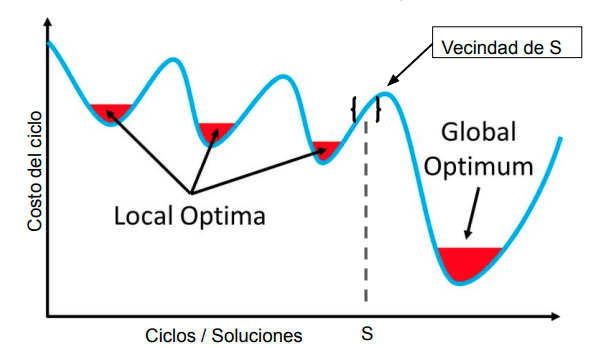
\includegraphics[width=0.5\textwidth]{img/tmp/busqueda-local.png}
    \caption{Esquema representativo del costo de cada ciclo en función de la relación ciclos sobre soluciones. Se puede observar la representación de óptimos locales (local optima), el óptimo global (global optimum) y las soluciones vecinas de $S$.}
    %\label{}
\end{figure}

Para intentar vencer esa limitación se desarrollaron las \textbf{metaheurísticas}, cuyo objetivo es realizar una búsqueda más amplia del espacio de soluciones, para así evitar caer en óptimos locales. Estas no son específicas para un problema dado, sino que son técnicas más generales utilizadas para construir heurísticas de búsqueda particulares para cada uno. La metaheurística implementada en este trabajo es \textbf{Tabú Search}

\subsection{Tabú Search}

La base del método es parecida a búsqueda local, comienza con una solución inicial y se mueve por su vecindad, pero contempla que a veces se necesita pasar por soluciones peores para llegar a soluciones mejores. El problema con esto es que puede llevar a ciclos, entonces para evitarlo hace uso de una \textbf{lista tabú}, que recuerda las soluciones previamente visitadas donde fue y no las exploras nuevamente. El esquema general del método es el descrito en el algoritmo \ref{alg:tabu-esquema}.

\begin{algorithm}[H]
    \begin{algorithmic}[1]
        \State{\textbf{Entrada:} los grafos $G$ y $H$ en representación de lista de adyacencia.}
        \State{\textbf{Salida:} coloreo y su impacto}
        \State
        \Function{TabuSearch}{$G$, $H$, ...}:
            \State actual $\gets$ \textbf{solucionInicial}(G, H) \Comment{$O(I)$}
            \State mejor $\gets$ actual
            \State T $\gets$ \textbf{inicializarMemoria(...)} \Comment{$O(T)$}
            
            \While{No se cumple el \textbf{criterio de parada}} \Comment{$O(\#it)$}
                \State actual $\gets$ $max$\{ filtrarTabu(\textbf{vecindad}(actual), T) \} \Comment{$O(|V| + N(s))$}
                \State T $\gets T + actual$ \Comment{$O(1)$}
                \If{impacto(actual) $>$ impacto(mejor)}
                    \State mejor $\gets$ actual
                \EndIf
            \EndWhile
            \State{\textbf{return} mejor, impacto(mejor)}
        \EndFunction
    \end{algorithmic}
    \caption{Esquema general de tabú search, en \textbf{negrita} cosas a definir. Las complejidades suponen accesos en tiempo constante a memoria}
    \label{alg:tabu-esquema}
\end{algorithm}

La complejidad entonces será $O(I + T + \#it \times (|V| + N(s))$, donde

\begin{itemize}
    \item \textbf{I} es el costo de obtener la solución inicial,
    \item \textbf{T} es el costo de inicializar la memoria,
    \item \textbf{$|V|$} es el tamaño de la vecindad, $max$ y $filtrarTabu$ son lineales en cuanto a ella,
    \item \textbf{N(s)} es el costo de encontrar la vecindad.
\end{itemize}

\subsubsection{Parámetros}

Como se puede ver en esquema general presentado en el Algoritmo \ref{alg:tabu-esquema}, el método varía según la elección de \textbf{solución inicial}, \textbf{memoria}, \textbf{criterio de parada} y \textbf{vecindad}. Se describen las versiones que se contemplan de cada uno.

\begin{itemize}
    \item \textbf{Solución inicial}: Se consideran como procedimientos para generar la solución inicial todas heurísticas constructivas golosas presentadas previamente: W, WP y S-LF.
    \item \textbf{Criterio de parada}: Se toma una cantidad máxima de iteraciones para el algoritmo.
    \item \textbf{Memoria}: Existen dos tipos. Por \textbf{solución} (i.e un coloreo) y \textbf{estructura}, en lugar de recordar las soluciones, se recuerdan los \textit{cambios estructurales} que llevaron de una a otra. En el segundo caso, podría causar que más de una solución que se obtenga con el mismo cambio se marque como tabú y no se visite. Incluso las no exploradas que podrían llegar a ser mejores, dado que el coloreo resultante de aplicar un cambio estructural depende del \textit{contexto} en el cuál se aplicó. El mismo cambio engloba a más de un coloreo. Para evitar perder buenas solucionas, se introduce la \textbf{función de aspiración}. Si una solución es tabú pero es mejor que lo visto hasta el momento, \textit{se aspira} y se la considera como solución factible. Esto es contemplado en \textit{filtrarTabu} del Algoritmo \ref{alg:tabu-esquema}.
    
    Es importante notar que la función de aspiración no tiene sentido junto con la memoria por soluciones, ya que si el algoritmo ya pasó por esa solución, fue contemplada ella y su vecindad en su totalidad, y no tendría sentido volver a verla.
    
    Además, la memoria tiene un tamaño fijo, ya que guardar el espacio entero de soluciones sería demasiado costoso.

    \item \textbf{Vecindad}: Se definen dos movimientos o cambios estructurales para pasar de una solución a otra: \textbf{change} (cambiar un color de un vértice por uno ya usado en el coloreo) y \textbf{swap} (intercambiar los colores de dos vértices). Finalmente, la vecindad de una solución será el conjunto de variaciones que presenten un coloreo válido luego de realizar un solo cambio. Opcionalmente, se puede tomar una parte de la vecindad para restringir la búsqueda e influenciar la toma de decisiones subóptimas. La representación de la estructura utilizada para almacenar en la memoria es en tuplas $(v, c) \mid v \in V, c$ color para $change$ y $(v, w) \mid v, w \in V$ para $swap$.
\end{itemize}

\subsection{Vecindades}

Los procedimientos para las vecindades a ser usados en las implementaciones concretas de Tabú Search son los siguientes:

\begin{algorithm}[H]
    \begin{algorithmic}[1]
        \Function{VecinosChange}{$G = (V, X_G)$, $H$, coloreo, ...} \Comment{$O(n^2 + n \times (m_G + m_H))$}
            \State vecinos $\gets \{\}$
            \For{v $\in$ V} \Comment{$O(n^2 + n \times (m_G + m_H))$}
                \State coloresAdy $\gets \{ coloreo[w] \mid (w, v) \in X_G\} \cup \{ coloreo[v] \}$ \Comment{$O(m_G)$}
                \State coloresFactibles $\gets coloreo \setminus coloresAdy$ \Comment{$O(n)$}
                \For{c $\in$ coloresFactibles}
                \State vecinos $\gets$ vecinos $\cup\ \{(coloreo[v] \twoheadleftarrow c, impacto(coloreo) + \Delta_I\}$ \Comment{$O(m_H)$} \label{alg-line:vecinos-twohead}
                \EndFor 
            \EndFor
            \State \textbf{return} vecinos
            \EndFor
        \EndFunction
        \Function{VecinosSwap}{$G = (V, X_G)$, $H$, coloreo, ...} \Comment{$O(n^2 + n \times (m_G + m_H))$}
            \State vecinos $\gets \{\}$
            \For{v $\in$ V} \Comment{$O(n^2 + n \times (m_G + m_H))$}
                \For{w $\in$ V}
                    \State $swapValido \gets \begin{aligned}[t]
                        &\nexists\ u \in N(v), coloreo[u] = coloreo[w]\ \wedge \\
                        &\nexists\ u \in N(w), coloreo[u] = coloreo[v]
                    \end{aligned}$  \Comment{$O(m_G)$}
                    \If{swapValido}
                        \State vecinos $\gets$ vecinos $\cup\ \{(swap(coloreo, v, w), impacto(coloreo) + \Delta_I\}$ \Comment{$O(m_H)$}
                    \EndIf
                \EndFor
            \EndFor
                
            \State \textbf{return} vecinos
            \EndFor
        \EndFunction
    \end{algorithmic}
    \caption{Procedimientos para distintas vecindades}
    \label{alg:tabu-proc-vecindad}
\end{algorithm}

Donde $\twoheadleftarrow$ en la línea \ref{alg-line:vecinos-twohead} de Change asigna el color al coloreo y devuelve el coloreo resultante. $\Delta_I$ es la diferencia de impacto resultante del cambio estructural. Para ambos casos, se calcula en $O(m_H)$ y está definido de la siguiente manera

$$\Delta_I = \#\{w \in N_H(v) \wedge c_w = c\} - \#\{w \in N_H(v) \wedge c_w = c_v\},$$

donde $c_v$ es el color del vértice $v$, $N_H(v)$ son los vértices adyacentes a él en $H$ y $c$ el nuevo color del vértice $v$.

El tamaño de ambas vecindades $|V|$ es $O(n^2)$, ya que para cada vértice se puede cambiar el color por todos los usados hasta el momento (a lo sumo $n$) o intercambiar con el resto (también $n$).

Para ambas, opcionalmente se puede especificar un \textbf{porcentaje} a tomar de la vecindad, para lo cual se mezcla la vecindad de forma aleatoria y se toma la primera fracción cuyo tamaño alcanza dicho porcentaje. Esto puede ayudar a que tabú explore más y tome soluciones peores que los óptimos locales.

\subsection{Variaciones}\label{ts-variaciones}

Finalmente, se presentan las variaciones de \textit{tabú search} implementadas en este trabajo. Para la complejidad, se deja sin determinar aquello que depende de meta parámetros no definidos, cada uno de los cuales será optimizado durante la experimentación. Por lo tanto, la complejidad es la misma para todos: $O(I + T + \#it \times (|V| + N(s)) = O(I + |T| + \#it \times (n^2 + n \times (m_G + m_H))$

\begin{itemize}
    \item \textbf{TSC-E}: Tabú Search con vecindades de \textit{change} y memoria de tipo estructura.
    \item \textbf{TSC-C}: Tabú Search con vecindades de \textit{change} y memoria de tipo solución (coloreo).
    \item \textbf{TSS-C}: Tabú Search con vecindades de \textit{swap} y memoria de tipo solución (coloreo).
    \item \textbf{TSS-E}: Tabú Search con vecindades de \textit{swap} y memoria de tipo estructura.
\end{itemize}

Cada clase de vecindad tiene una desventaja. Para \textbf{change}, como se cambia el color de un vértice por otro ya utilizado en el coloreo, en cada paso la cantidad de colores pasa a ser menor o igual. Esto hace que el espacio de soluciones al que se puede llegar desde la vecindad de la solución actual se reduzca en cada iteración hasta que no haya más vecinos. Por lo tanto, ciertas soluciones muy cerca del óptimo no se podrían explorar mucho y el algoritmo terminaría cortando luego de pocas iteraciones. En cambio, resulta evidente que algoritmos que den soluciones razonables, pero no con la mínima cantidad de colores, pueden hacer que el algoritmo performe mejor. Por otro lado, en \textbf{swap} pasa lo contrario. Al intercambiar los colores de dos vértices, la cantidad de colores se mantiene luego de cada iteración, por lo que se cree que puede ser más conveniente tener como solución inicial un coloreo de pocos colores. Visto en términos de los algoritmos descritos, probablemente sea conveniente que comience con $S-LF$ o $WP$ en vez de $W$, ya que dan soluciones con menos colores. Estas suposiciones se validarán experimentalmente.
\section{Experimentación}

 % hilo de la exp:
 % 1. heur golosas
 % 2. analisis de cual va a ser el impacto de los parms sobre tabu
 % 3. desarmar el impacto de cada parametro
 % 4. resultados, ranking, evaluacion general

\subsection{Metodología experimental}\label{section:metodologia-experimental}

El objetivo de la experimentación es lograr comparar el desempeño de los distintos algoritmos para diferentes parámetros, contrastando tiempo de ejecución con calidad de soluciones. Para ello, se define un conjunto de instancias de tamaños variados ($n = [6, 8..., 30]$) para las cuales se conoce el valor óptimo, separado en instancias de \textit{train} (entrenamiento, $n \not\equiv 0\ (\text{mod}\ 4)$) y \textit{test} (verificación, $n \equiv 0\ (\text{mod}\ 4)$). De esta forma, se buscan los mejores parámetros en las instancias de \textit{train} y luego se verifica si efectivamente son los mejores comparándolos con instancias del conjunto de \textit{test}.

\subsubsection{Rangos para parámetros de Tabú Search}

Para correr todas las combinaciones de las variaciones descritas en la sección \ref{ts-variaciones} sobre las instancias de \textit{train}, se definen los siguientes rangos para los parámetros de Tabú Search:

\begin{itemize}
    \item \% vecindad $\in \{5, 10, \dots, 30, 40, \dots, 100\}$
    \item $|T|$ (\textit{tamaño de la memoria}) $\in \{5, 20, \dots, 65, 100, 200, \dots 600\}$
    \item $\#iteraciones \in \{100, 300, \dots, 900\}$
    \item aspirar $\in \{si, no\}$.
\end{itemize}

\subsubsection{Métricas}

Para medir la eficiencia se usa el tiempo de ejecución, y para la calidad de las soluciones el \textit{gap relativo} con respecto de la solución óptima, definido de la siguiente manera:

$$\text{gap relativo} = \frac{I(x) - I(x^*)}{I(x^*)},$$

\textit{donde $I$ calcula el impacto de una solución $x$ y $x^*$ es alguna óptima.}

\subsubsection{Especificaciones técnicas}

Los algoritmos fueron implementados utilizando el lenguaje de programación $C++$, y fueron ejecutados en una computadora con un Intel(R) Core(TM) i5-4460 CPU @ 3.20GHz (32K cache lvl 1, 256K lvl 2 y 6MB lvl 3) y 16GB de RAM.

\subsection{Heurísticas constructivas golosas}

Se comenzó evaluando el desempeño de las distintas heurísticas constructivas golosas para distintas instancias del problema PCMI. En la \cref{plot:heuristicas constructivas} izquierda se puede observar que, en líneas generales, el $gap$ relativo promedio aumenta con el tamaño de la instancia para todas las heurísticas constructivas golosas implementadas. Este resultado es esperable porque a mayor tamaño de instancia es más probable que un algoritmo goloso tome una decisión local que afecte negativamente la calidad de la solución futura y, por su naturaleza, esta decisión no es reevaluada. Se observan también oscilaciones en la calidad de la solución que pueden deberse a particularidades topológicas de cada instancia.

Como se menciona en la Sección \ref{metodologia}, la heurística WP es una mejora de la heurística W. Los resultados obtenidos en la \cref{plot:heuristicas constructivas} soportan está observación, dado que para todas las instancias evaluadas el gap relativo promedio es menor para WP que para W. A su vez, como la mejora de WP respecto de W está asociada a intentar colorear vértices que W no colorearía, esto requiere corroborar la factibilidad de dicha decisión en cada caso. En la \cref{plot:heuristicas constructivas} derecha, se observa que esto implica un aumento en el tiempo promedio de ejecución de WP respecto de W. Sin embargo, la diferencia parece ser despreciable.

\begin{figure}[H]
    \centering
    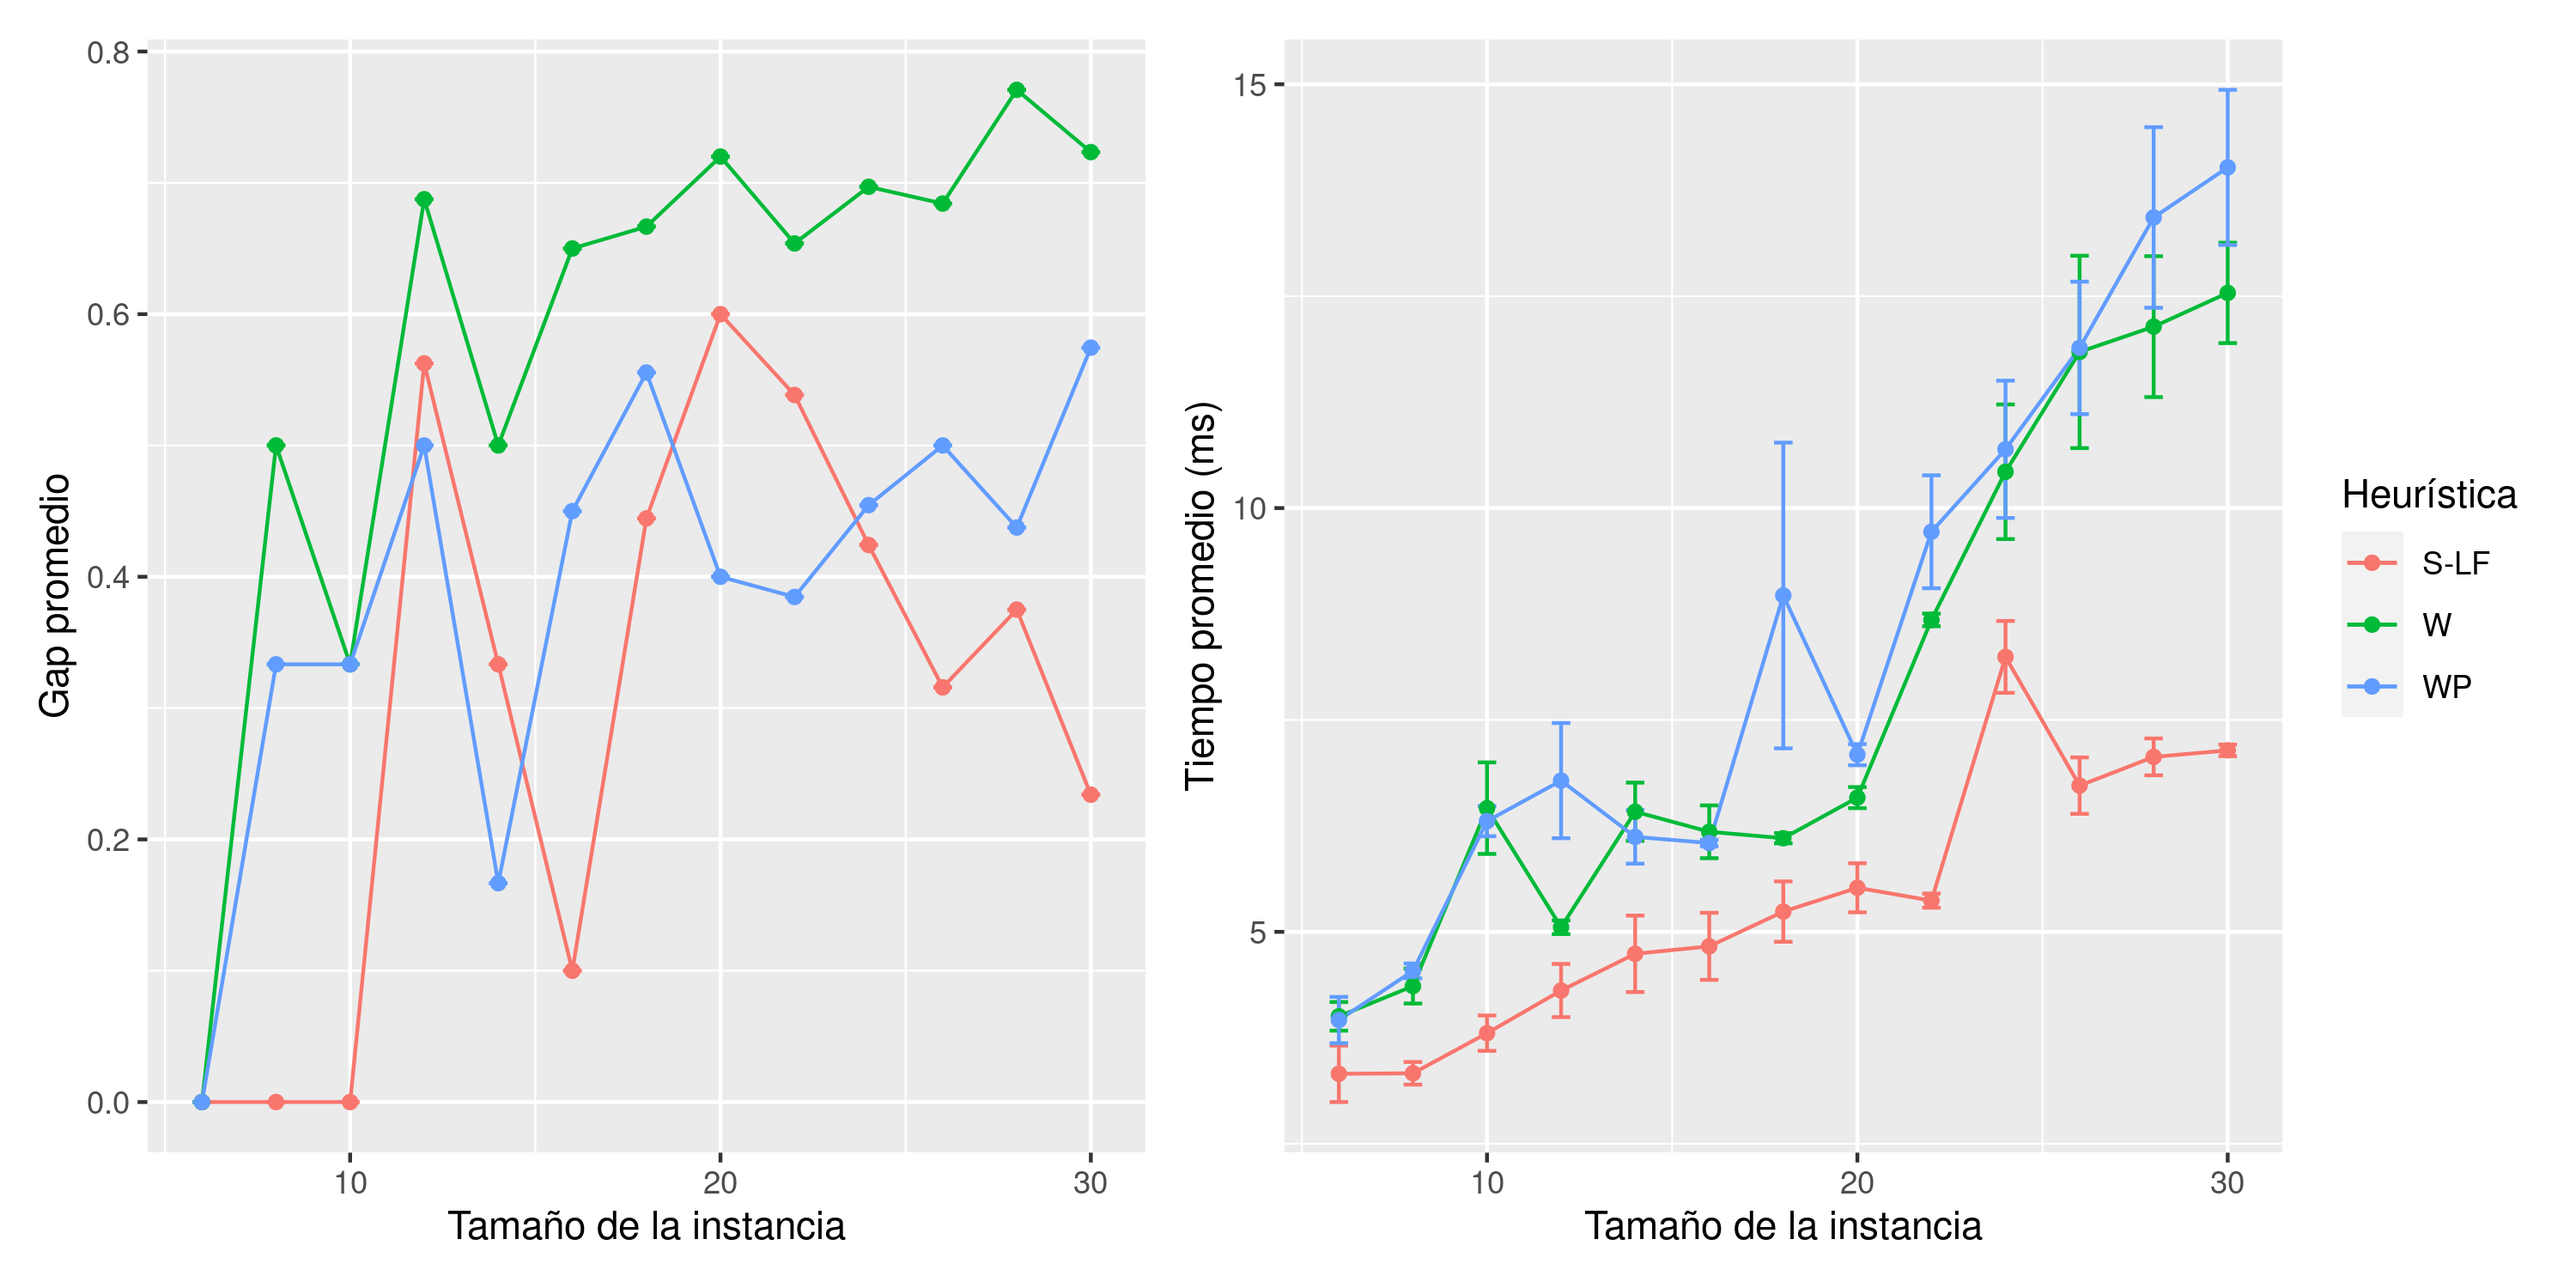
\includegraphics[width=.9\textwidth]{plots/heuristicas_constructivas.png}
    \caption{Gap relativo promedio en función del tamaño de la instancia (izq.) y tiempo promedio de ejecución en función del tamaño de la instancia. Los puntos representan el valor medio y las barras el error estándar. Se realizaron 5 repeticiones por instancia.}
    \label{plot:heuristicas constructivas}
\end{figure}

Por otro lado, también se observa que para muchas instancias el desempeño de WP y SL-F parece ser comparable. Sin embargo, para tamaños de instancia muy chicos y muy grandes S-LF parece ser mejor. Una posible explicación para las instancias de mayor tamaño es que como WP busca aumentar el impacto evaluando vértices de a pares, dependiendo del orden de evaluación de los vértices conectados en H, podría ocurrir que se generen subgrupos de vértices con colores distintos. Esto no pasaría en S-LF ya que minimiza la cantidad de colores, aumentando así el impacto como consecuencia y desconociendo las relaciones presentes en H. Finalmente, se puede observar que el tiempo de ejecución de SL-F es mucho menor al de las otras dos heurísticas constructivas golosas. 

\begin{figure}[H]
    \centering
    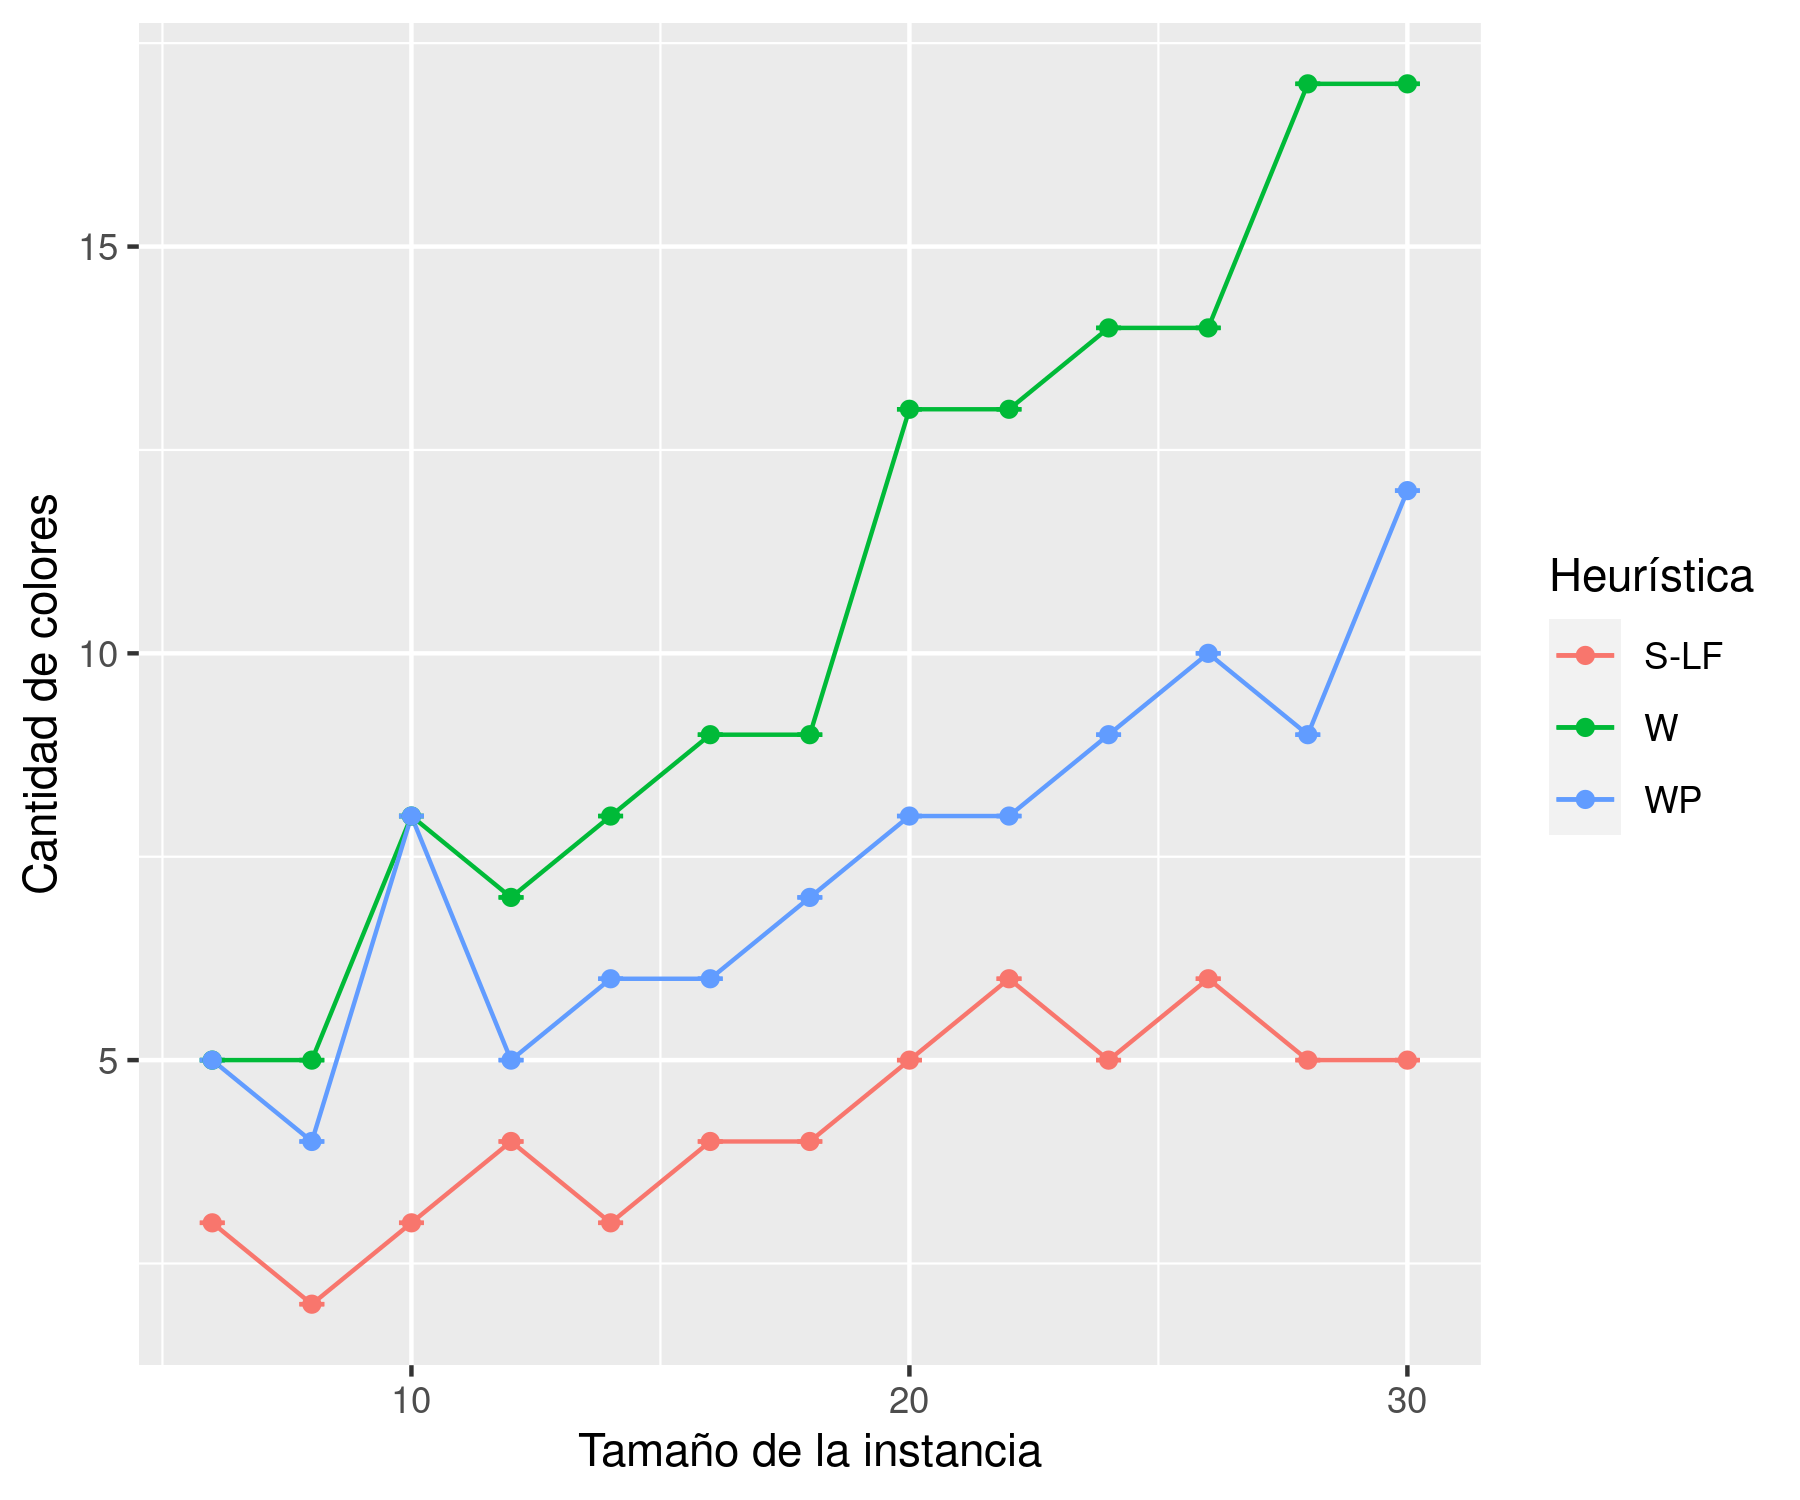
\includegraphics[width=0.6\textwidth]{plots/heuristicas_constructivas_colores.png}
    \caption{Cantidad de colores de la solución obtenida en función del tamaño de la instancia para las distintas heurísticas constructivas golosas. Se realizaron 5 repeticiones por instancia.}
    \label{plot:heuristicas constructivas colores}
\end{figure}

En la \cref{plot:heuristicas constructivas colores} se corrobora que, para cada tamaño de instancia, la cantidad de colores de la solución obtenida es mayor para W, intermedia para WP y menor para S-LF.

Teniendo en cuenta los resultados de esta sección, se concluye que S-LF es la mejor heurística constructiva golosa en términos de distancia respecto del óptimo y tiempo de ejecución. Sin embargo, esto no implica que necesariamente sea la mejor heurística inicial para todas las metaheurísticas y parámetros posibles porque la cantidad de coloreos de la solución inicial podría tener un impacto importante sobre la posibilidad de generar vecinos, dependiendo de la estrategia empleada por cada metaheurística.

\subsection{Impacto de parámetros}

De acuerdo a lo concluido en la sección anterior, se evaluó a cada metaheurística partiendo de la solución proporcionada por cada una de las heurísticas constructivas golosas. Adicionalmente, para cada una de estas combinaciones, se variaron los parámetros de las metaheurísticas como se describe en la sección \ref{section:metodologia-experimental} con el objetivo de poder encontrar una configuración óptima. Para esto sólo se utilizaron las instancias de entrenamiento.

\begin{figure}[H]
    \centering
\begin{subfigure}[b]{0.7\textwidth}
         \centering
         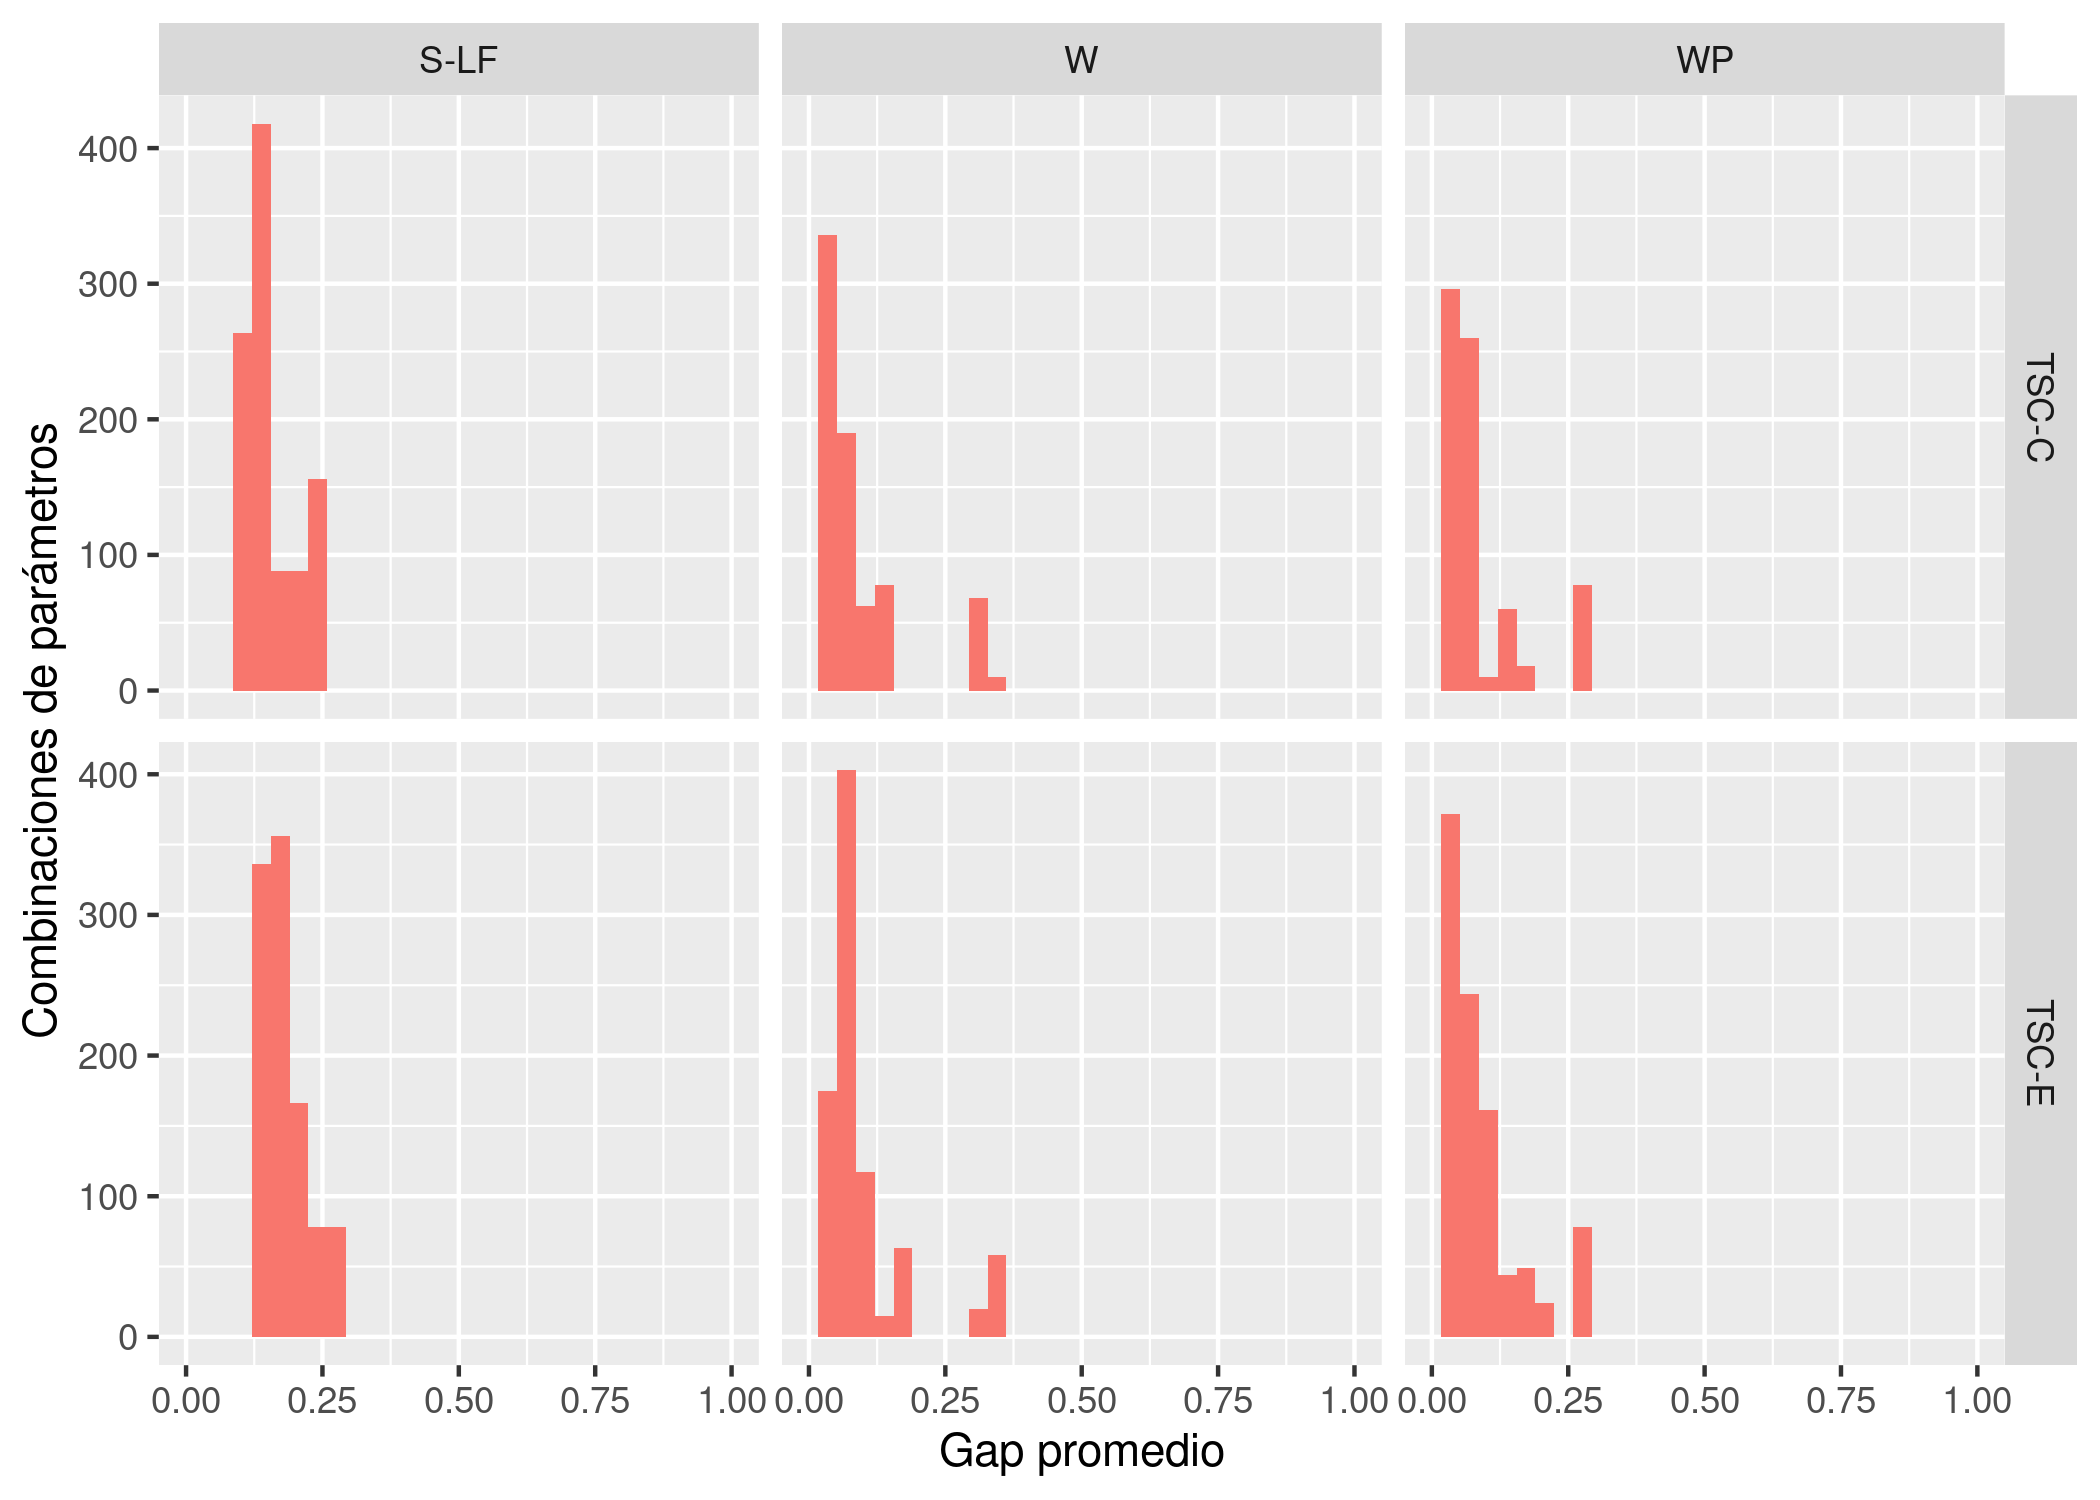
\includegraphics[width=\textwidth]{plots/histograma_tsc.png}
         \label{fig:histogramas-TSC}
\end{subfigure}
\begin{subfigure}[b]{0.7\textwidth}
         \centering
         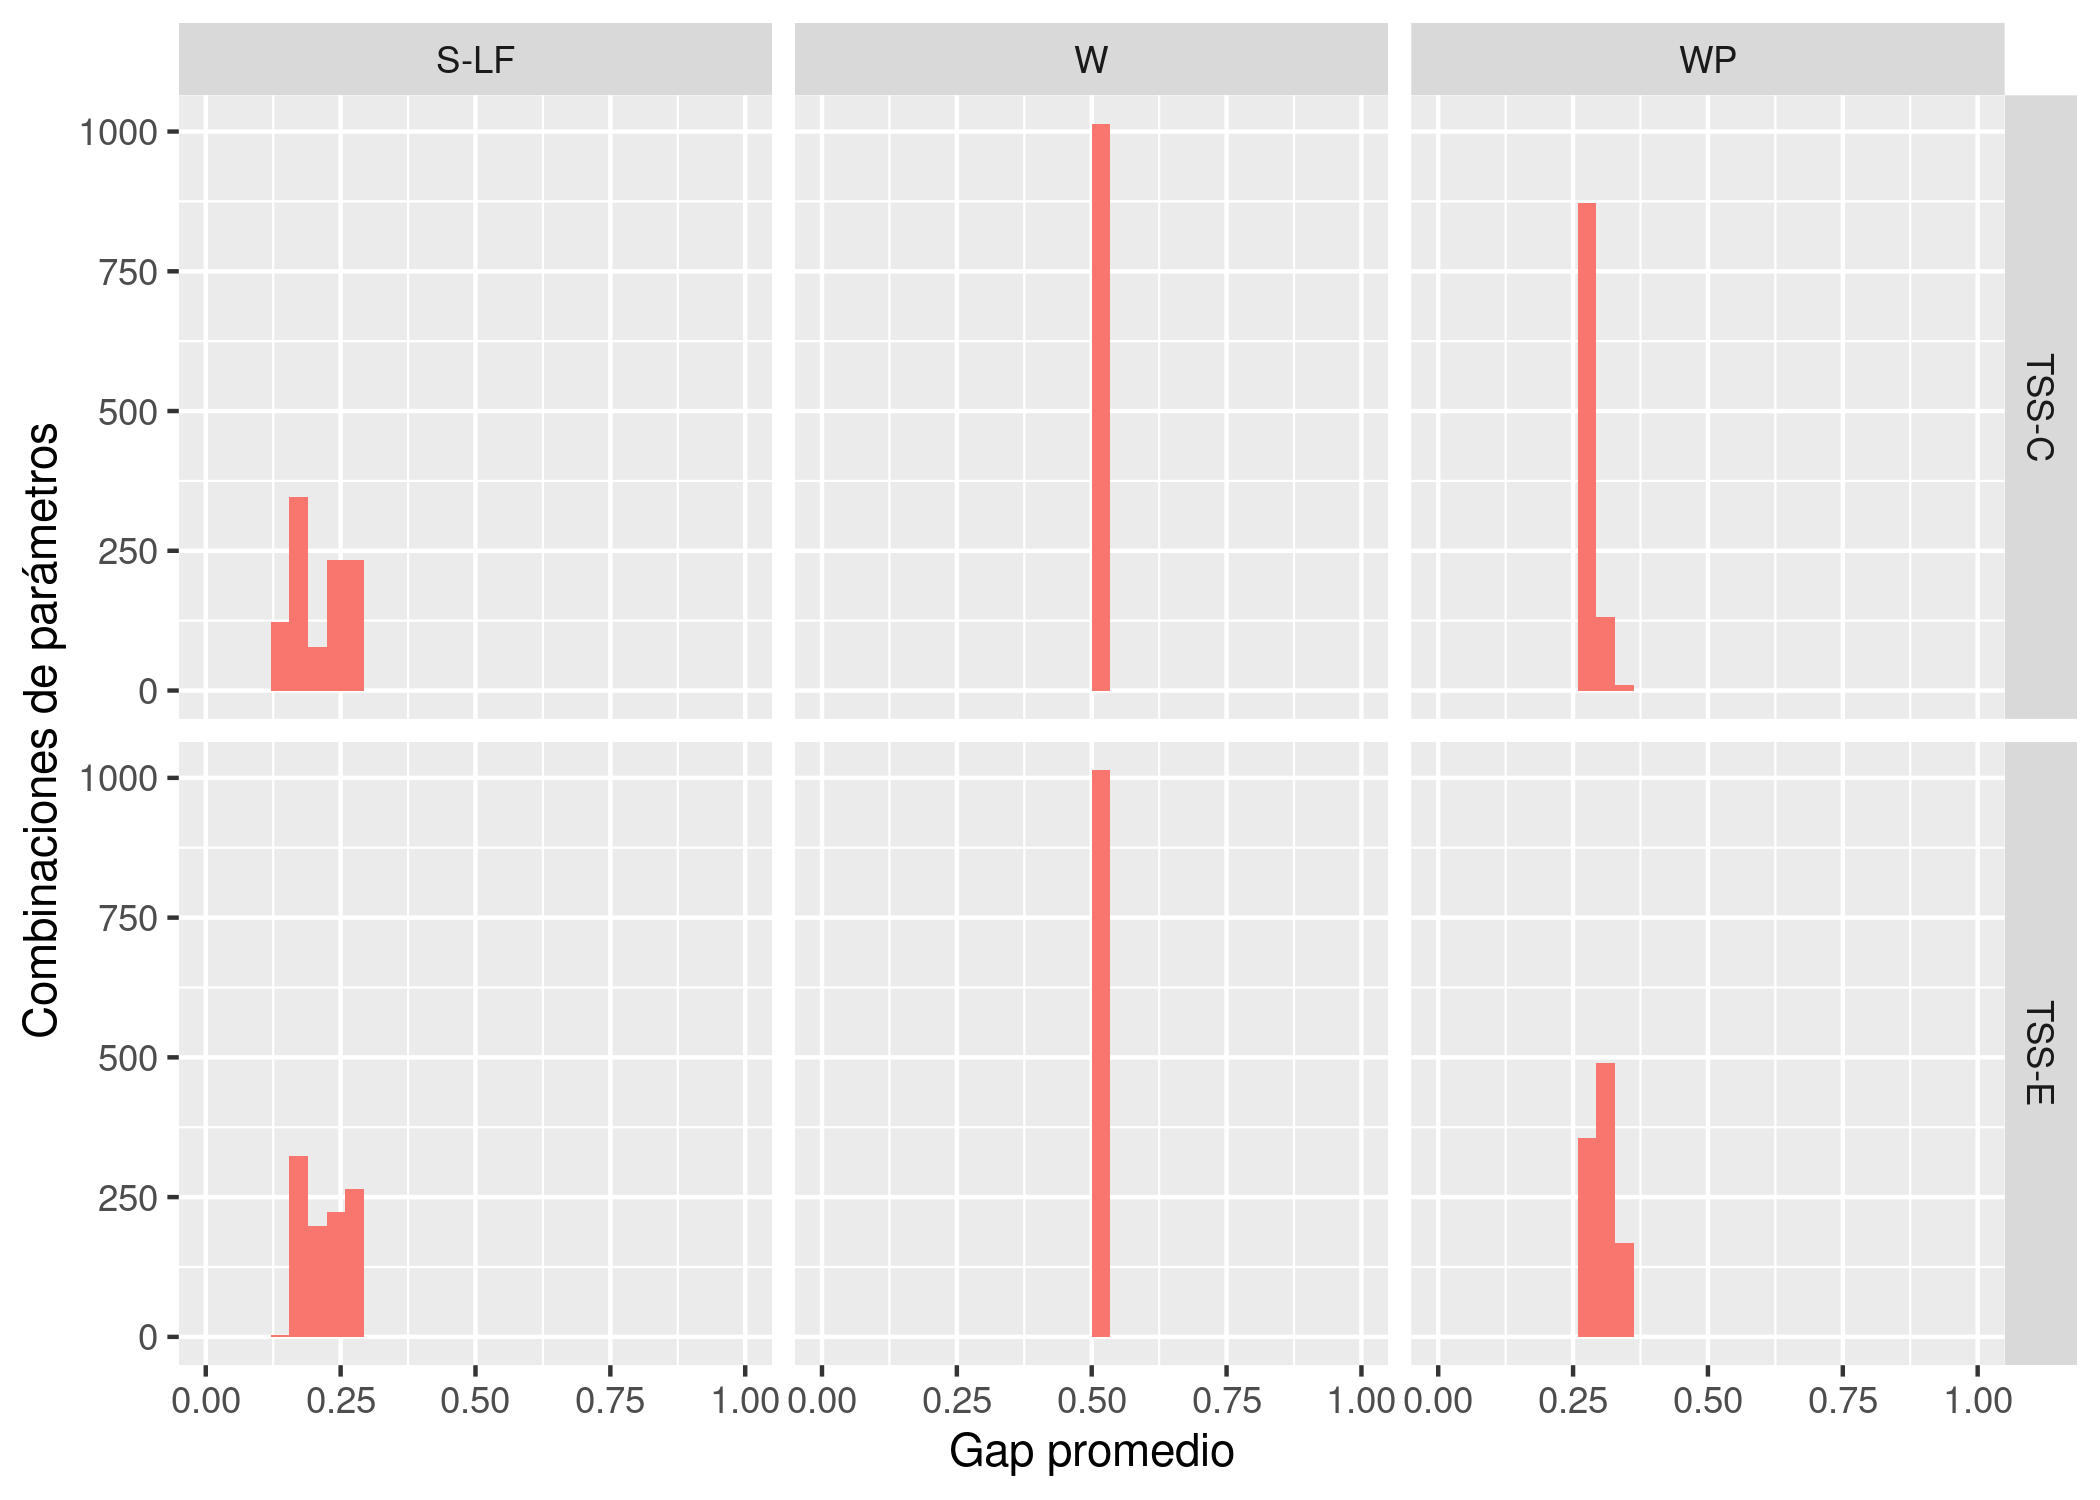
\includegraphics[width=\textwidth]{plots/histograma_tss.png}
         \label{fig:histogramas-TSS}
\end{subfigure}
\caption{Histogramas que indican la cantidad de combinaciones de parámetros que resultan en un mismo valor de gap relativo promedio. En la parte superior, se muestran los resultados obtenidos para las variaciones de Tabú search que usan vecindades generadas por la metodología \textbf{change} (TSC) y, en parte inferior, los resultados obtenidos para las variaciones que usan vecindades generadas por la metodología \textbf{swap} (TSS). A su vez, cada una está dividida en paneles según el tipo de memoria usada (C por coloreo y E por estructura) y la heurística constructiva inicial empleada (S-LF, W o WP).}
\label{plot:histogramas}
\end{figure}

En la \cref{plot:histogramas} se muestran, en la parte superior, los resultados obtenidos para las variaciones de Tabú search que usan vecindades generadas por la metodología \textbf{change} (TSC) y, en parte inferior, los resultados obtenidos para las variaciones que usan vecindades generadas por la metodología \textbf{swap} (TSS). A su vez, cada una está dividida en paneles según el tipo de memoria usada (C por coloreo y E por estructura) y la heurística constructiva inicial empleada (S-LF, W o WP). En cada panel se grafica un histograma que indica la cantidad de combinaciones de parámetros que resultan en un mismo valor de gap relativo promedio.

En líneas generales, a pesar de los amplios rangos de los parámetros evaluados, se observa una gran cantidad de combinaciones de los mismos que dan resultados equivalentes. En la siguientes secciones se intentará comprender por qué ocurre esto.

Más allá de esto, para TSC (figura superior) se observa un rango de variación en la calidad de la solución ocasionado por la variación de los parámetros independientemente del tipo de memoria y de la heurística constructiva inicial. Adicionalmente, para esta metodología de construcción de vecindad, parece ser peor la heurística constructiva S-LF que WP y W, ya que para estás últimas dos el mejor gap está más cerca de $0$. Sin embargo, existen combinaciones de parámetros que permiten obtener resultados comparables entre todos los tipos de heurísticas constructivas golosas para TSC.

En el caso de TSS (figura inferior) la variación en la calidad de la solución es más reducida y es dependiente de la heurística constructiva inicial. Se observan grandes diferencias de gap promedio que parecen depender más de la heurística inicial que de los parámetros. A pesar de esto, se puede concluir que, en el caso de emplear la heurística constructiva S-LF, parece haber lugar para la optimización de parámetros y posiblemente en el caso de WP también. Para esta metodología de generación de vecinos, parece ser mejor la heurística S-LF que W y WP ya que el mejor $gap$ está más cerca de 0 para S-LF. Adicionalmente, no existe combinación de parámetros que logre resultados competitivos para W y WP respecto de S-LF.

Para analizar el impacto de variar cada parámetro sobre el desempeño de las metaheurísticas y tratar de comprender por qué distintas combinaciones de los mismos pueden resultar equivalentes, se decidió empezar evaluando el efecto de variar el porcentaje de vecindad.

\subsection{Impacto del porcentaje de vecindad}

Dados los resultados vistos en la sección anterior, resultó interesante comenzar a analizar cada parámetro en particular para intentar dilucidar el impacto de cada uno en el desempeño de los algoritmos. Se comenzó analizando el efecto de tomar distintos tamaños de vecindad, ya que esto podría implicar cambios notables en el comportamiento del algoritmo. Para tamaños de vecindad baja, podría suceder que se ignoren mejoras de impacto que formen parte de la vecindad pero hayan quedado fuera por estar tomando una porción demasiado pequeña. Por el contrario, tomar la totalidad de la vecindad podría resultar en un estancamiento en óptimos locales.

En la \cref{plot:porcentaje vecindad} se puede observar una fuerte variación en los resultados al variar el porcentaje de vecindad. Respecto a TSC se puede ver que tomar una vecindad más grande resulta más provechoso, encontrando sus óptimos en los valores del rango $70 - 100$. Por el contrario, tomar una vecindad demasiado pequeña parece restringir demasiado las posibilidades de movimiento, inhabilitando posibles soluciones vecinas mejores.

Respecto de TSS se puede observar que algunos algoritmos como TSS-C-WP y TSS-E-WP encuentran óptimos para porcentajes de vecindad medianos. Se corrobora que TSS sólo varía el gap promedio de forma relevante cuando la heurística inicial es S-LF. Para la heurística WP la variación es mucho menor y para W es inexistente. Esto lleva a pensar junto con lo visto en la subfig. \ref{fig:histogramas-TSS}, que los algoritmos de \textit{Tabú Search Swap} no ofrecen mejoría alguna para el algoritmo inicial W, estancándose siempre en el impacto obtenido por la solución inicial. Sólo ofrecen mejoras leves para el algoritmo inicial WP.
 
Lo observado en esta sección permite concluir que el cambio del porcentaje de vecindad puede explicar en gran medida la variación del gap vista en la fig. \ref{plot:histogramas}, mostrando así la injerencia de este parámetro en la calidad de las soluciones obtenidas por el algoritmo. Por este motivo, se decidió evaluar el impacto de los parámetros restantes teniendo en cuenta el porcentaje de vecindad empleado.

\begin{figure}[H]
    \centering
    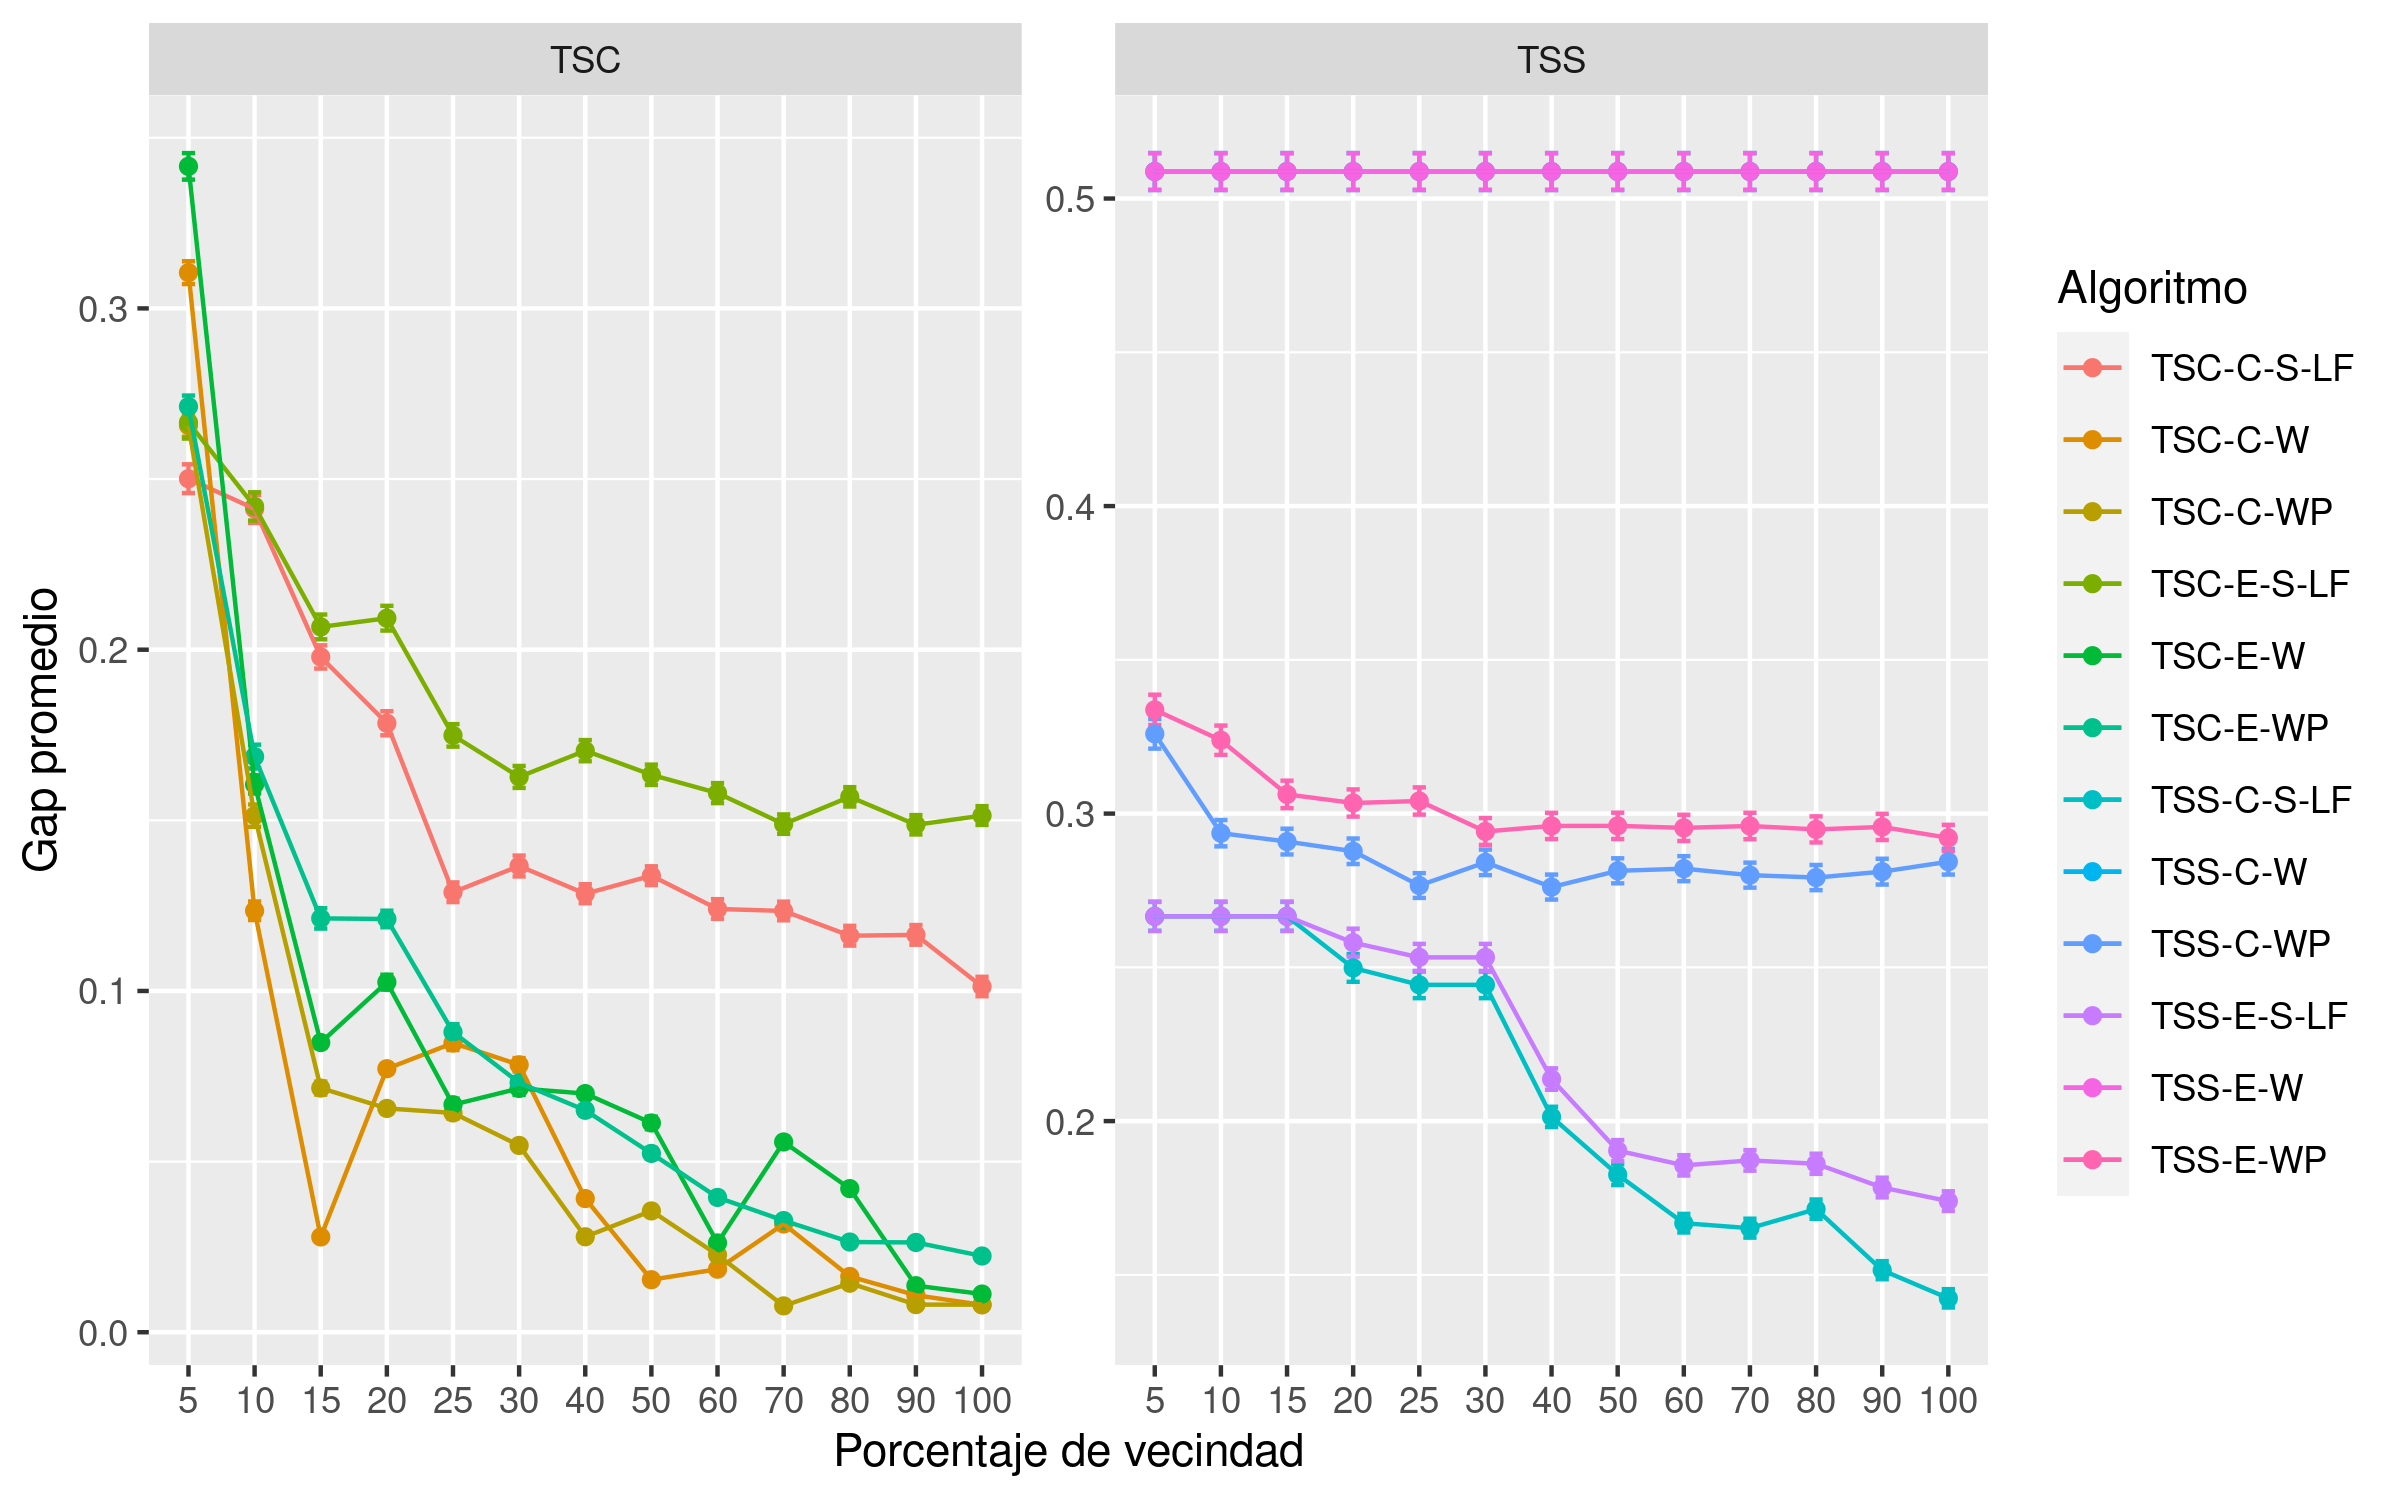
\includegraphics[width=0.8\textwidth]{plots/porcentaje_vecindad.png}
    \caption{{Gap promedio según combinación de algoritmo de Tabú Search con algoritmo goloso inicial para diferentes porcentajes de vecindad.}}
    \label{plot:porcentaje vecindad}
\end{figure}

\subsection{Impacto de aspirar}

Otro de los metaparámetros cuyo análisis resultó importante fue la utilización de una función de aspiración. Para ello, se corrieron los diferentes métodos de Tabú con un algoritmo goloso inicial óptimo para cada uno. Los resultados de TSS no presentaron diferencia alguna en la utilización de la función de aspiración para ninguna estructura de memoria.

\begin{figure}[H]
    \centering
    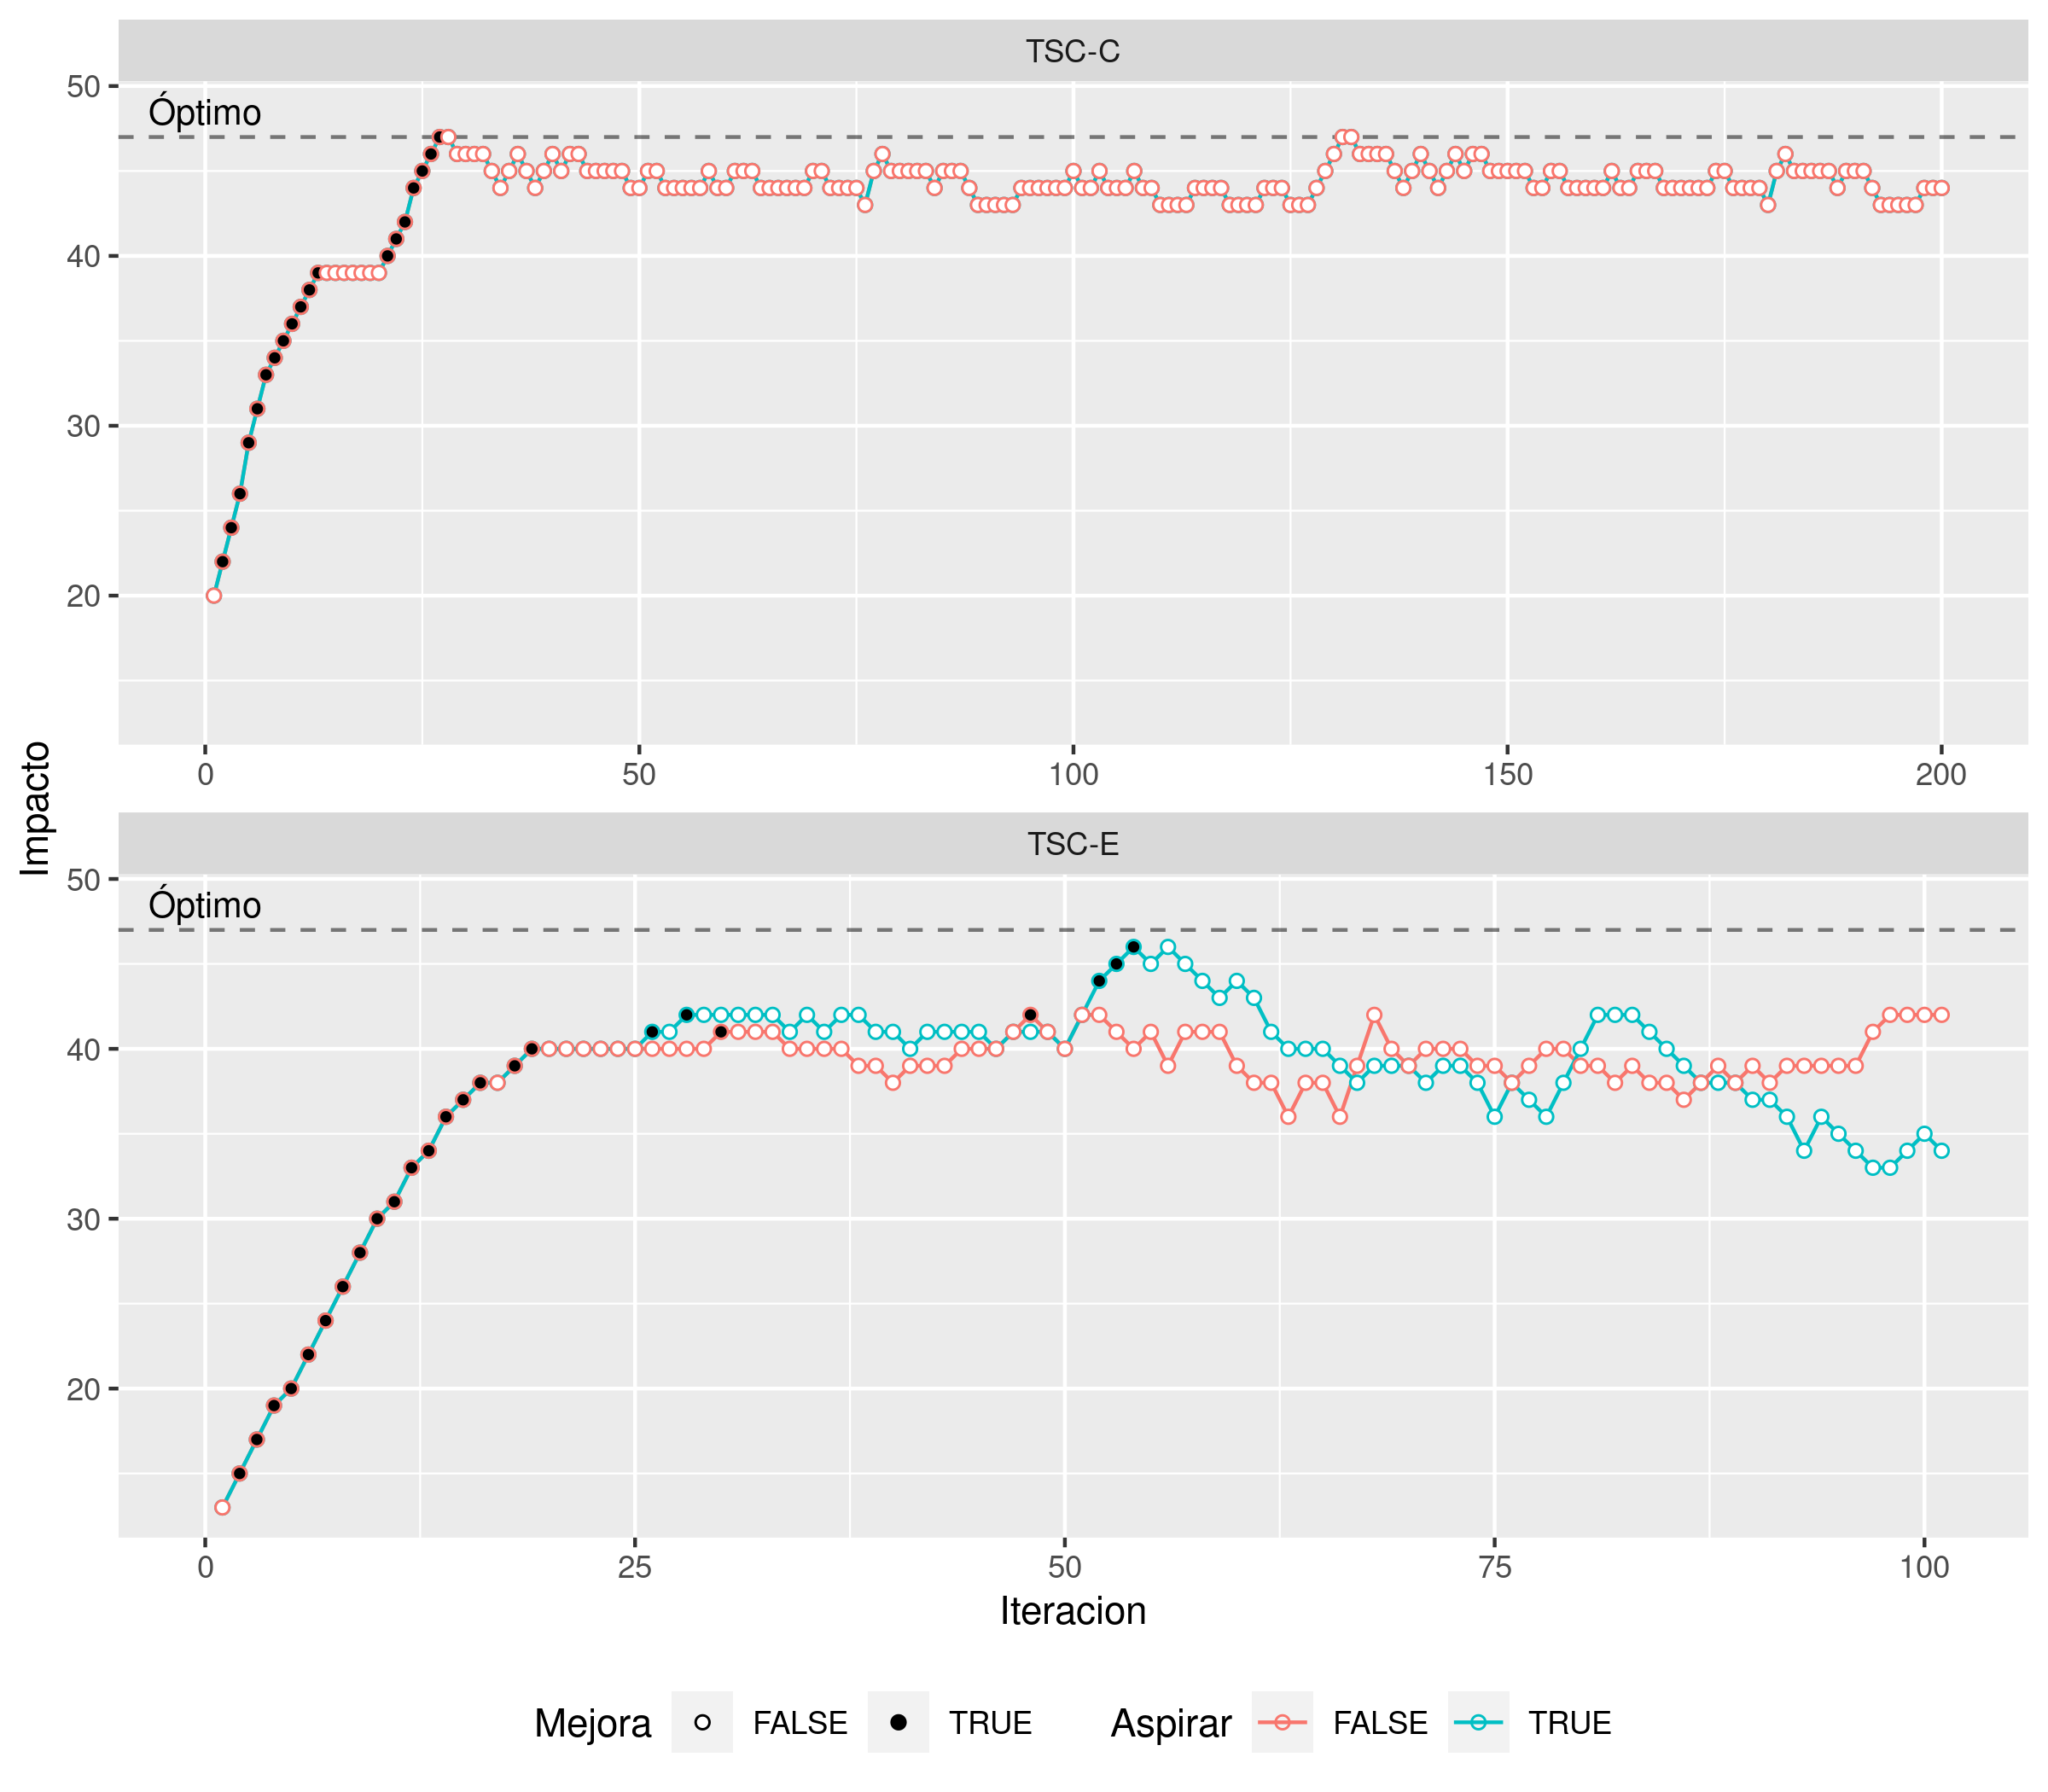
\includegraphics[width=0.7\textwidth]{plots/impacto_tiempo.png}
    \caption{Se observa el impacto en función del número de iteraciones para los algoritmos TSC-C Y TSC-E. Se observan en rojo los casos evaluados con función de aspiración y, en azul, aquellos que no. Los círculos rellenos implican que se observa una mejora en el impacto. Se realizaron 5 repeticiones por instancia.}
    \label{plot:impacto vs iteracion}
\end{figure}

Para el algoritmo TSC se observan dos situaciones diferentes. En el caso de utilizar una memoria por estructura se pueden obtener mejores resultados a partir de la función de aspiración. Esto se debe a que volver a utilizar un cambio de color en un vértice específico en un futuro coloreo distinto puede permitir una mejoría en el impacto de la solución, ya que dos coloreos radicalmente distintos (y con distinto impacto) pueden ser vecinos del mismo cambio estructural. En este sentido, la utilización de la función de aspiración permite desbloquear muchas soluciones posibles que permiten impactos distintos.

En el caso de utilizar una memoria por coloreo, aspirar no presenta ninguna diferencia con no hacerlo. Esto se condice con lo dicho anteriormente, ya que al haber pasado por un coloreo específico, se contemplan esa solución y sus vecinas. Luego, volver a pasar por esa situación no presenta nuevas oportunidades de coloreo que permitan una mejoría en el impacto. A su vez, resulta muy poco probable que un coloreo sufra los suficientes cambios como para pasar por una solución y luego volver exactamente al mismo coloreo. En este sentido, la probabilidad de volver a un coloreo exacto anterior resulta muy baja y no presenta ninguna mejoría, por lo que la función de aspiración no genera cambios en el impacto obtenido por esta implementación.

Finalmente, considerando la mejoría que brinda la función de aspiración, el costo temporal que ésta requiere resulta tolerable, por lo que resulta provechoso utilizarla. Esto puede verse en mayor profundidad en las figuras \ref{plot:aspirar tiempo tsc}, \ref{plot:aspirar tiempo tss}, \ref{plot:aspirar tsc} y \ref{plot:aspirar tss}.
 
\subsection{Impacto de tamaño de memoria}

En el paradigma computacional, los recursos de memoria y tiempo suelen ser elementos cuya optimización puede llevar a resultados considerablemente mejores. En el caso de los algorítmos metaheurísticos, la memoria y el tiempo resultan de vital importancia para un correcto funcionamiento. Sin embargo, se debe evitar el abuso de los mismos para no sumar gastos innecesarios. Por ello, se decidió establecer un rango amplio de memoria \ref{metodologia} y luego verificar cuánta era realmente necesaria para llegar a una buena solución.

Se corrió cada combinación de algoritmos Tabú con heurísticos iniciales y se graficó cada uno según porcentaje de vecindad. A su vez, se agregó una línea vertical con la cantidad de iteraciones efectivas\footnote{Iteraciones realmente efectuadas que terminaron antes de llegar al tope de iteraciones asignadas al algoritmo.} realizadas y sus respectivas barras de error, lo que permitió analizar en detalle la real utilización de la memoria.

\begin{figure}[H]
    \centering
    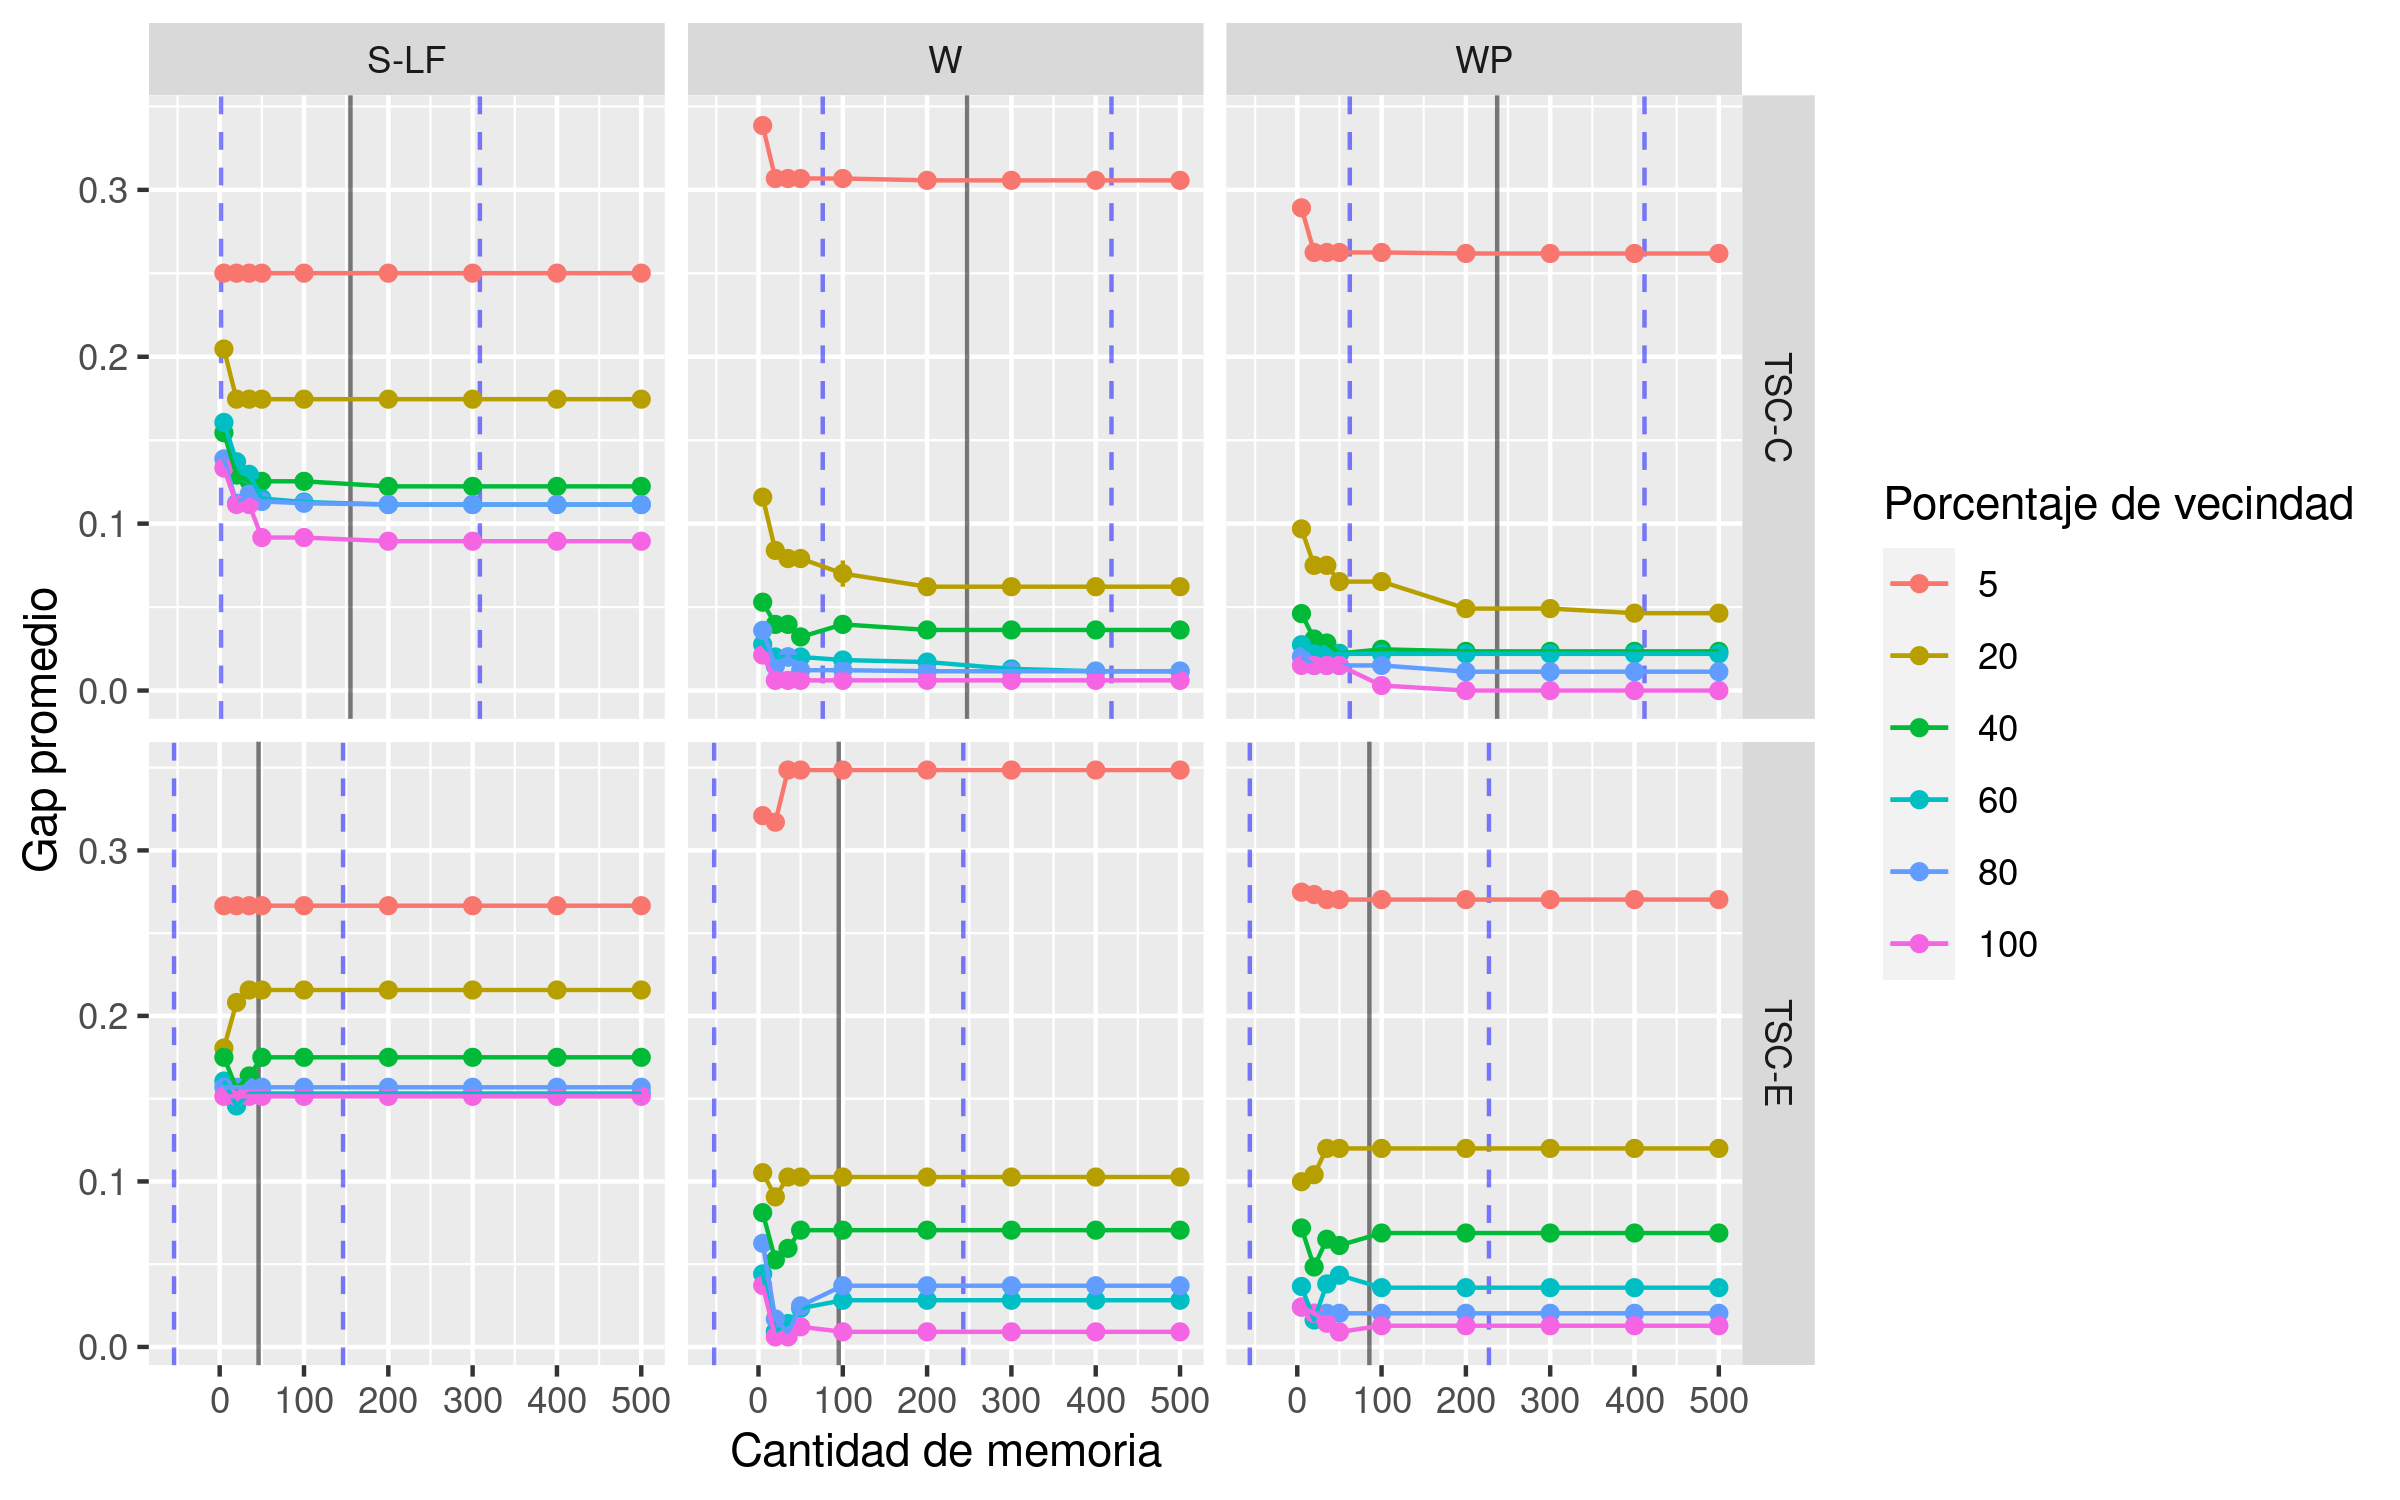
\includegraphics[width=0.8\textwidth]{plots/memoria_tsc.png}
    \caption{Gap promedio según cantidad de memoria asignada para cada combinación de algoritmo. Se grafican líneas verticales con iteraciones efectivas realizadas por cada algoritmo.}
    \label{plot:memoria tsc}
\end{figure}

En el caso de TSC, se puede observar que las iteraciones efectivas hacen que memoria no se use, lo que indica que no hace falta tanta memoria en algunos algoritmos. A su vez, no se notan cambios significativos en el gap para memoria mayor a 200 aproximadamente, lo que parecería mostrar que no es necesaria una gran cantidad de memoria para mantener una zona tabú efectiva.

A su vez, entre las dos diferentes estructuras de TSC (TSC-E y TSC-C) se ven diferencias en las iteraciones efectivas, realizando TSC casi el doble en promedio.  Esto podría deberse a lo explicado anteriormente, ya que al no recortar tanto la vecindad por la zona tabú definida en base a coloreo, se precisan más iteraciones para analizar la vecindad hasta quedarse sin vecinos o terminarse las iteraciones.

Respecto a los algoritmos iniciales elegidos, se puede observar que W y WP funcionan de manera similar en TSC-C y TSC-E pero S-LF no. Esto se debe a que la lógica del \textit{change} genera un nuevo vecino a partir de colores pre-existentes en el grafo no presentes en sus adyacentes. Por lo tanto, sólo puede mantener o disminuir el número de colores en el grafo. En consecuencia, al partir de una heurística golosa que minimiza la cantidad de colores\footnote{Notar que minimizar la cantidad de colores pensando únicamente en G puede ser contraproducente porque tener impacto implica repetir colores en H.}, la cantidad de soluciones posibles que puede explorar el algoritmo se ve reducida afectando negativamente a su performance.

\begin{figure}[H]
    \centering
    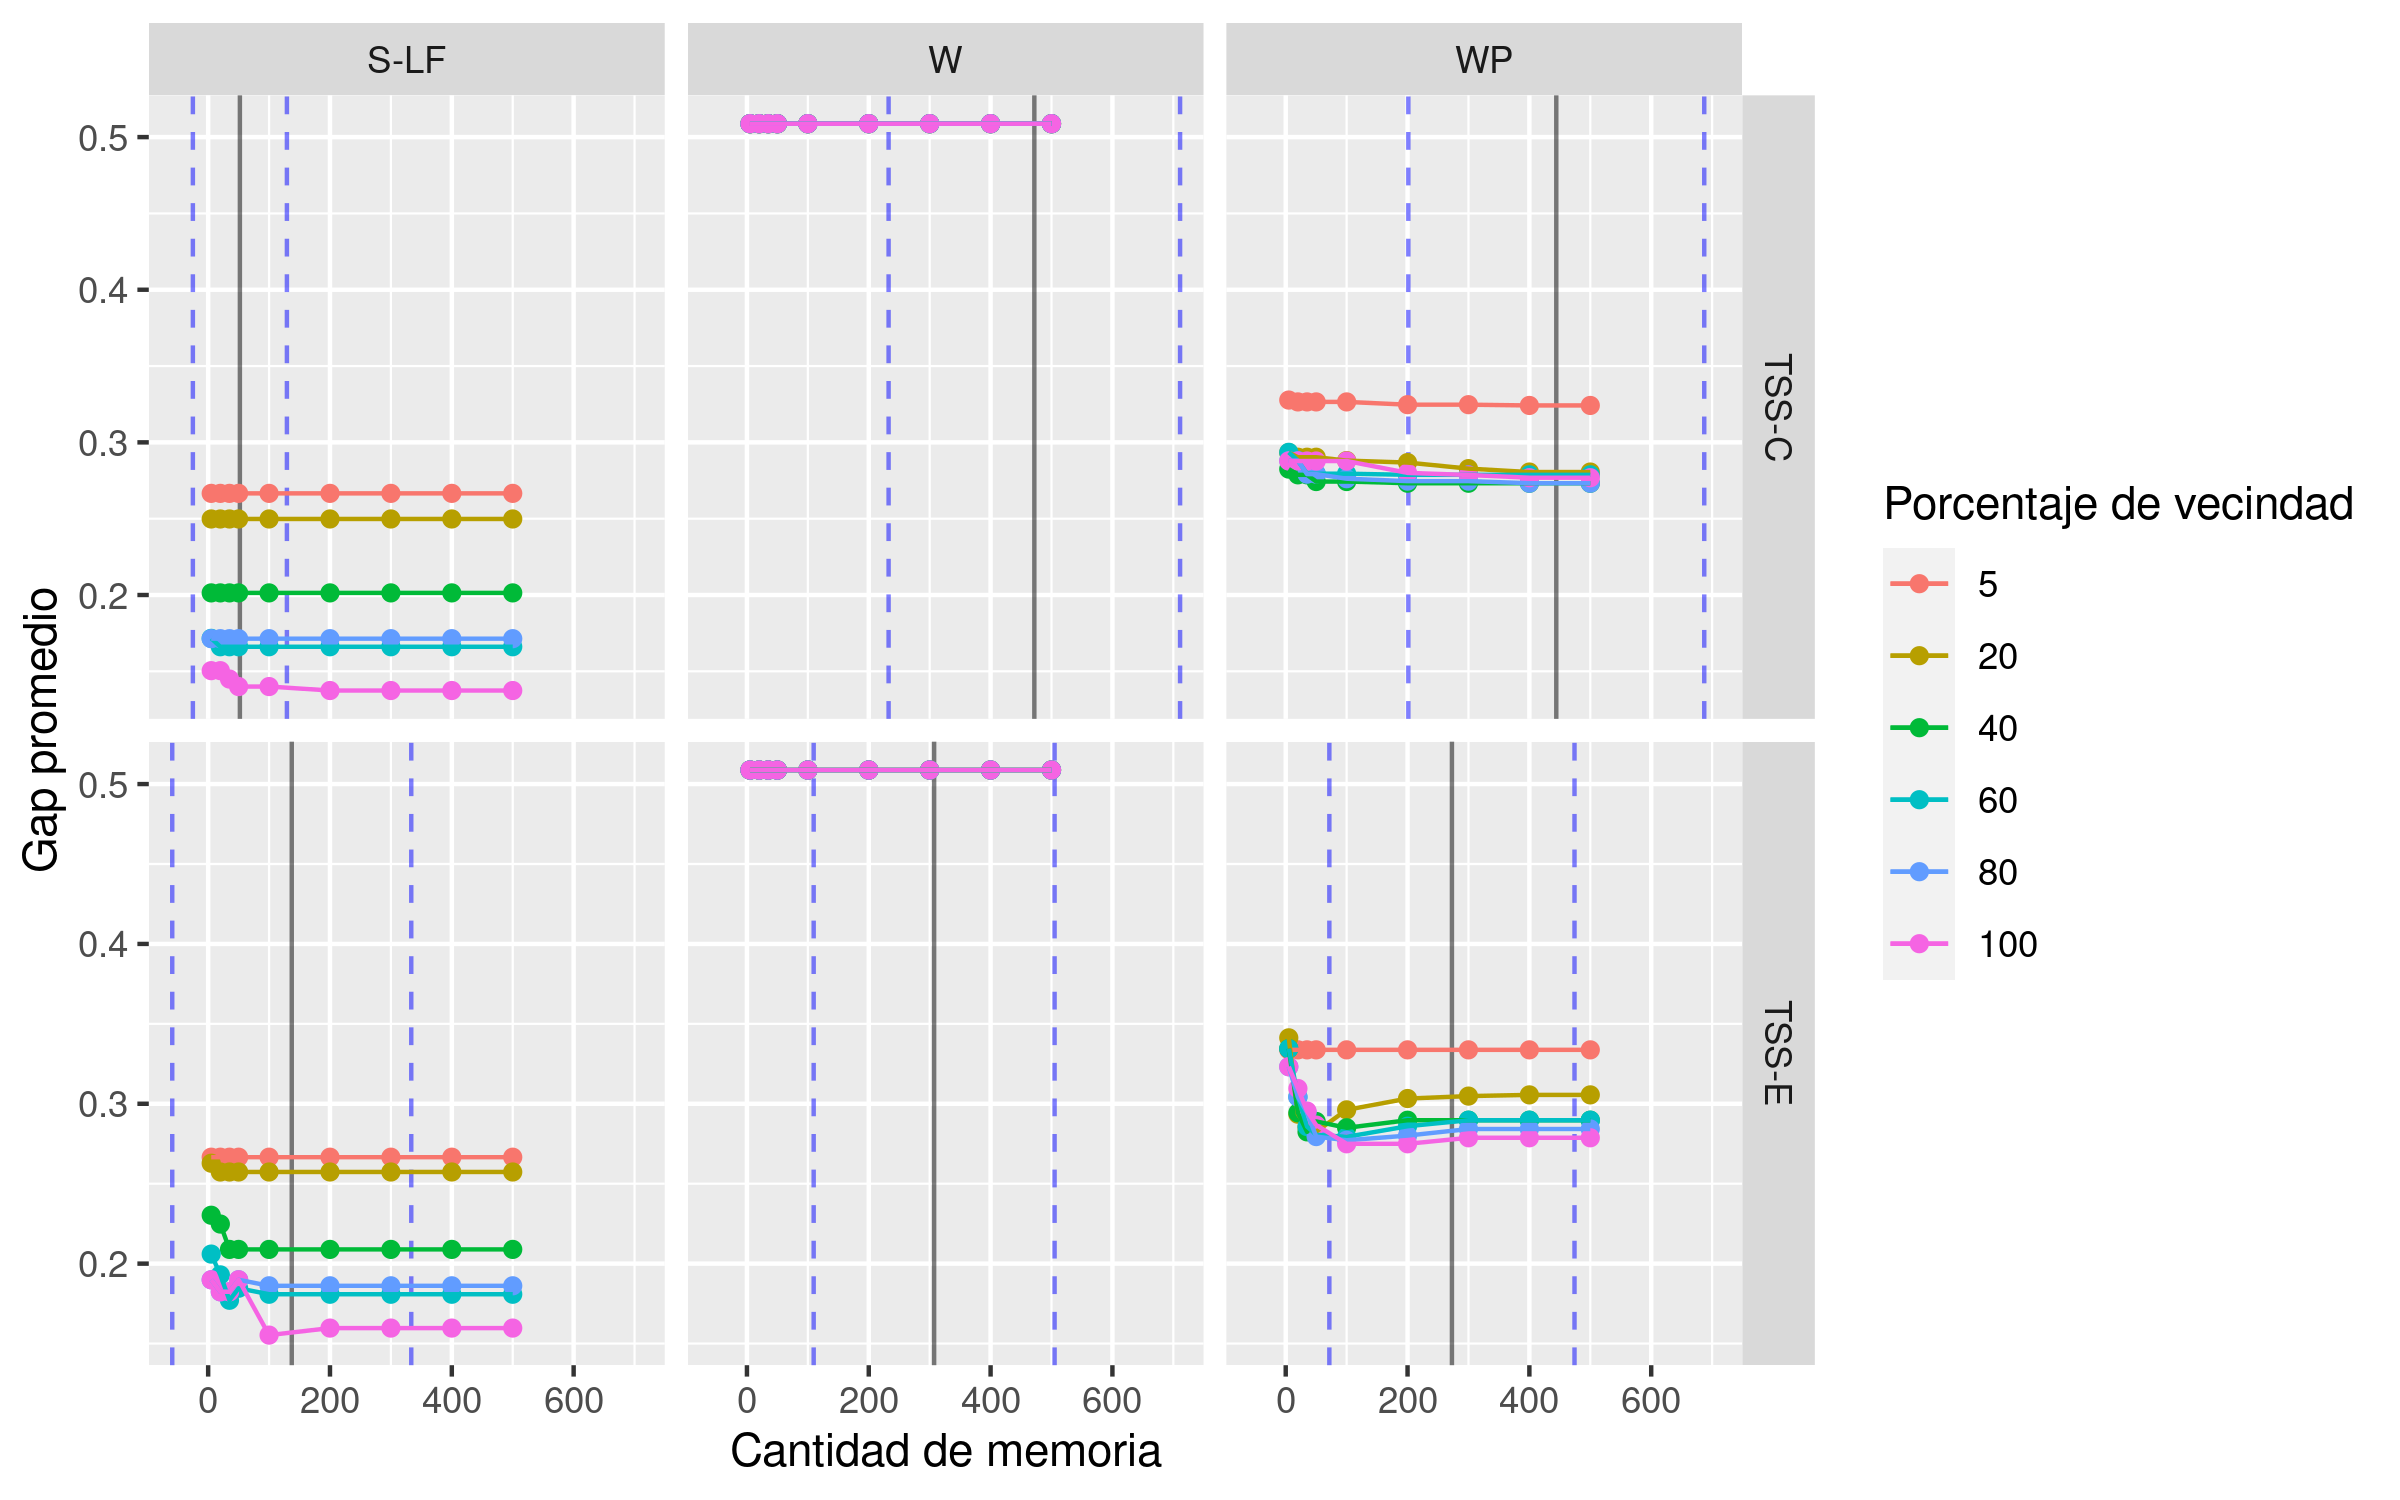
\includegraphics[width=0.8\textwidth]{plots/memoria_tss.png}
    \caption{Se observa el gap promedio en función de la cantidad de memoria para todas las combinaciones de tabú search swap y los algoritmos heurísticos iniciales. En todos los casos, se grafican los resultados obtenidos para valores de porcentaje de vecindad en [5, 20, 40, 60, 80, 100]. Se realizaron 5 repeticiones por instancia.}
    \label{plot:memoria tss}
\end{figure}

A primera vista, para TSS utilizando los algoritmos iniciales W y WP parecería tener sentido usar una gran cantidad de memoria, ya que no estaría siendo anulada por la cantidad de iteraciones. Sin embargo, para W la performance no cambia respecto de este parámetro, descartando esta posibilidad. En este caso, lo que sucede es que hay gran vecindad que la memoria no es capaz de cubrir completamente, por lo que siempre habrá vecinos para analizar (aunque no mejoren el impacto). Esto sucede porque la heurística golosa W utiliza muchos colores. Luego, como TSS sólo intercambia colores (no introduce nuevos) de vértices y W utiliza muchos colores, la vecindad resulta muy grande y la memoria no logra acapararla toda, por lo que el algoritmo prácticamente se detiene cuando se queda sin iteraciones. A su vez, es por este mismo motivo que el desempeño del algoritmo es malo. Al no tener muchos colores repetidos y no puede introducir nuevos, no logra tener un alto impacto ni tampoco mejorarlo, llegando a su óptimo rápidamente y estancándose en él.

En el caso de WP, la heurística golosa reduce la cantidad de colores en las componentes conexas de H pero no limita la cantidad en los vértices aislados en H, generando una cantidad de colores intermedia que da una vecindad de tamaño intermedio. Por otro lado S-LF reduce la cantidad de colores en general, causando una mayor reducción del número de colores y en consecuencia de la vecindad. Esto explica por qué las iteraciones efectivas decrecen en el orden W, WP, S-LF y la performance aumenta en el mismo sentido.

\subsection{Impacto de cantidad de iteraciones}

Según lo visto en la sección anterior, resultaría lógico ver una gran diferencia entre las iteraciones asignadas a cada algoritmo y las efectivas. Para verificar esto se analizaron las diferentes combinaciones de algoritmos y se graficó el gap promedio según la cantidad de iteraciones. Al igual que antes se agregó una línea vertical que indica las iteraciones efectivas.

\begin{figure}[H]
    \centering
    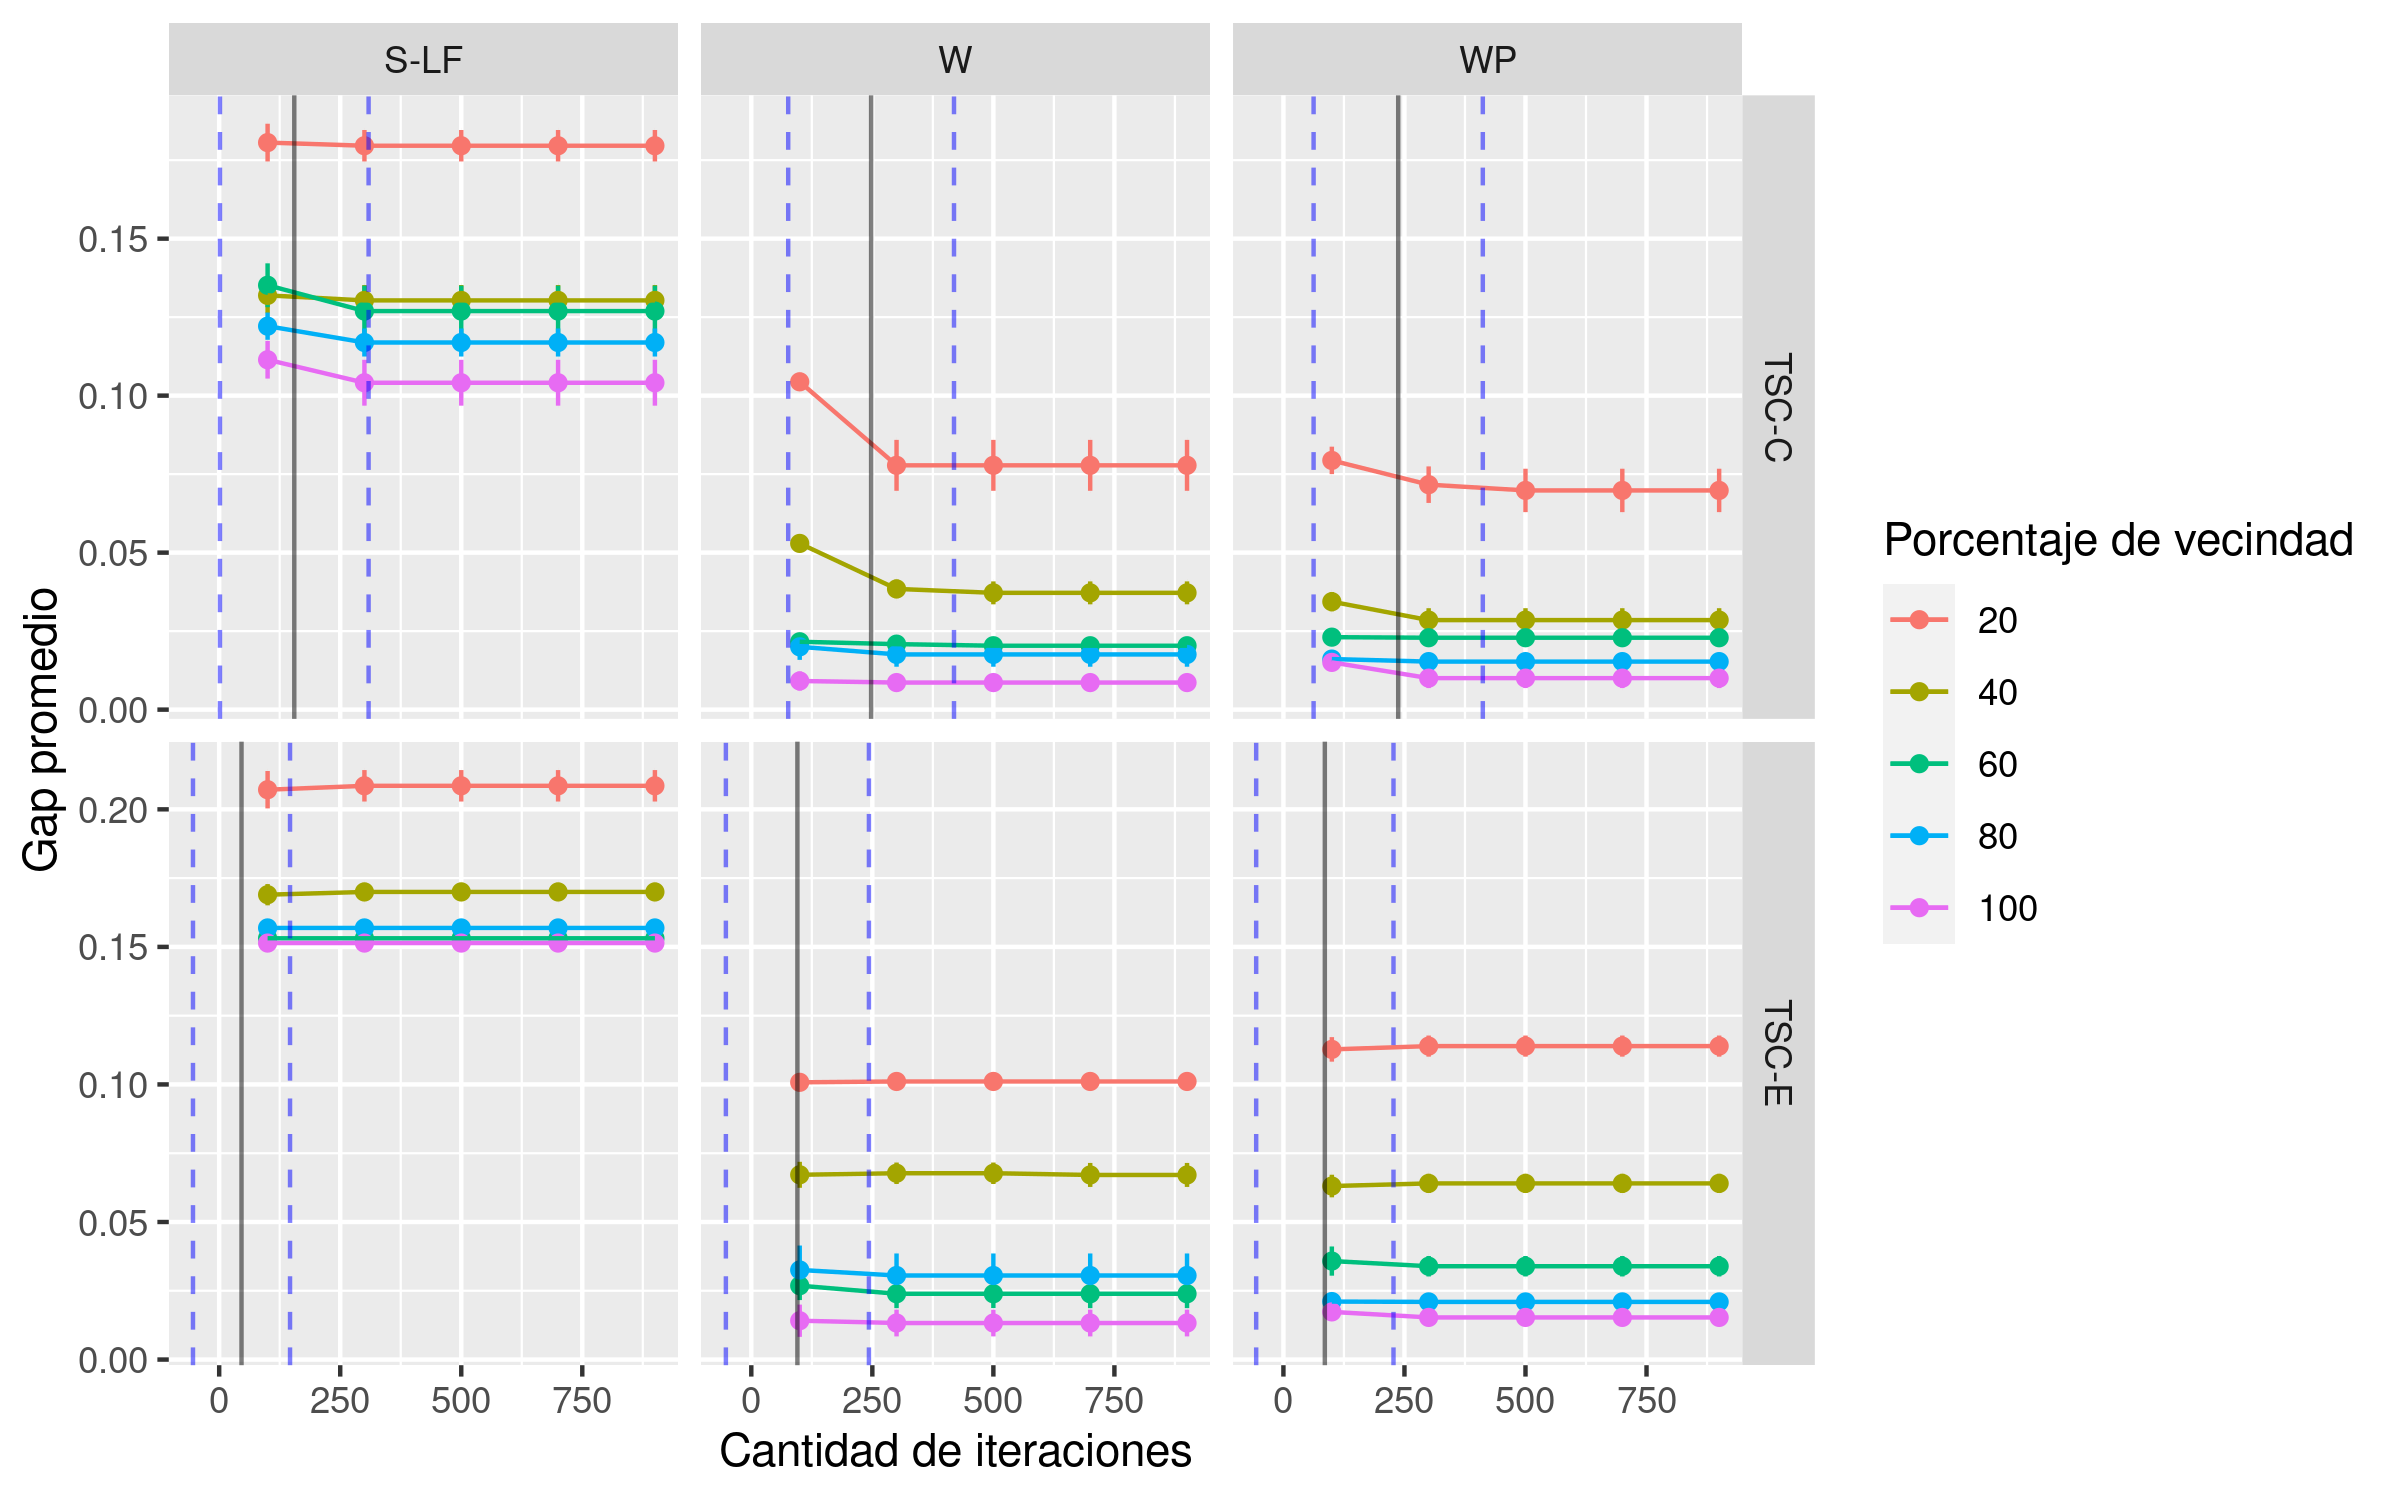
\includegraphics[width=0.8\textwidth]{plots/iteraciones_tsc.png}
    \caption{Se observa el gap promedio en función de la cantidad de memoria para todas las combinaciones de tabú search change y los algoritmos heurísticos iniciales. En todos los casos, se grafican los resultados obtenidos para valores de porcentaje de vecindad en [5, 20, 40, 60, 80, 100]. Se realizaron 5 repeticiones por instancia.}
    \label{plot:iteraciones tsc}
\end{figure}

\begin{figure}[H]
    \centering
    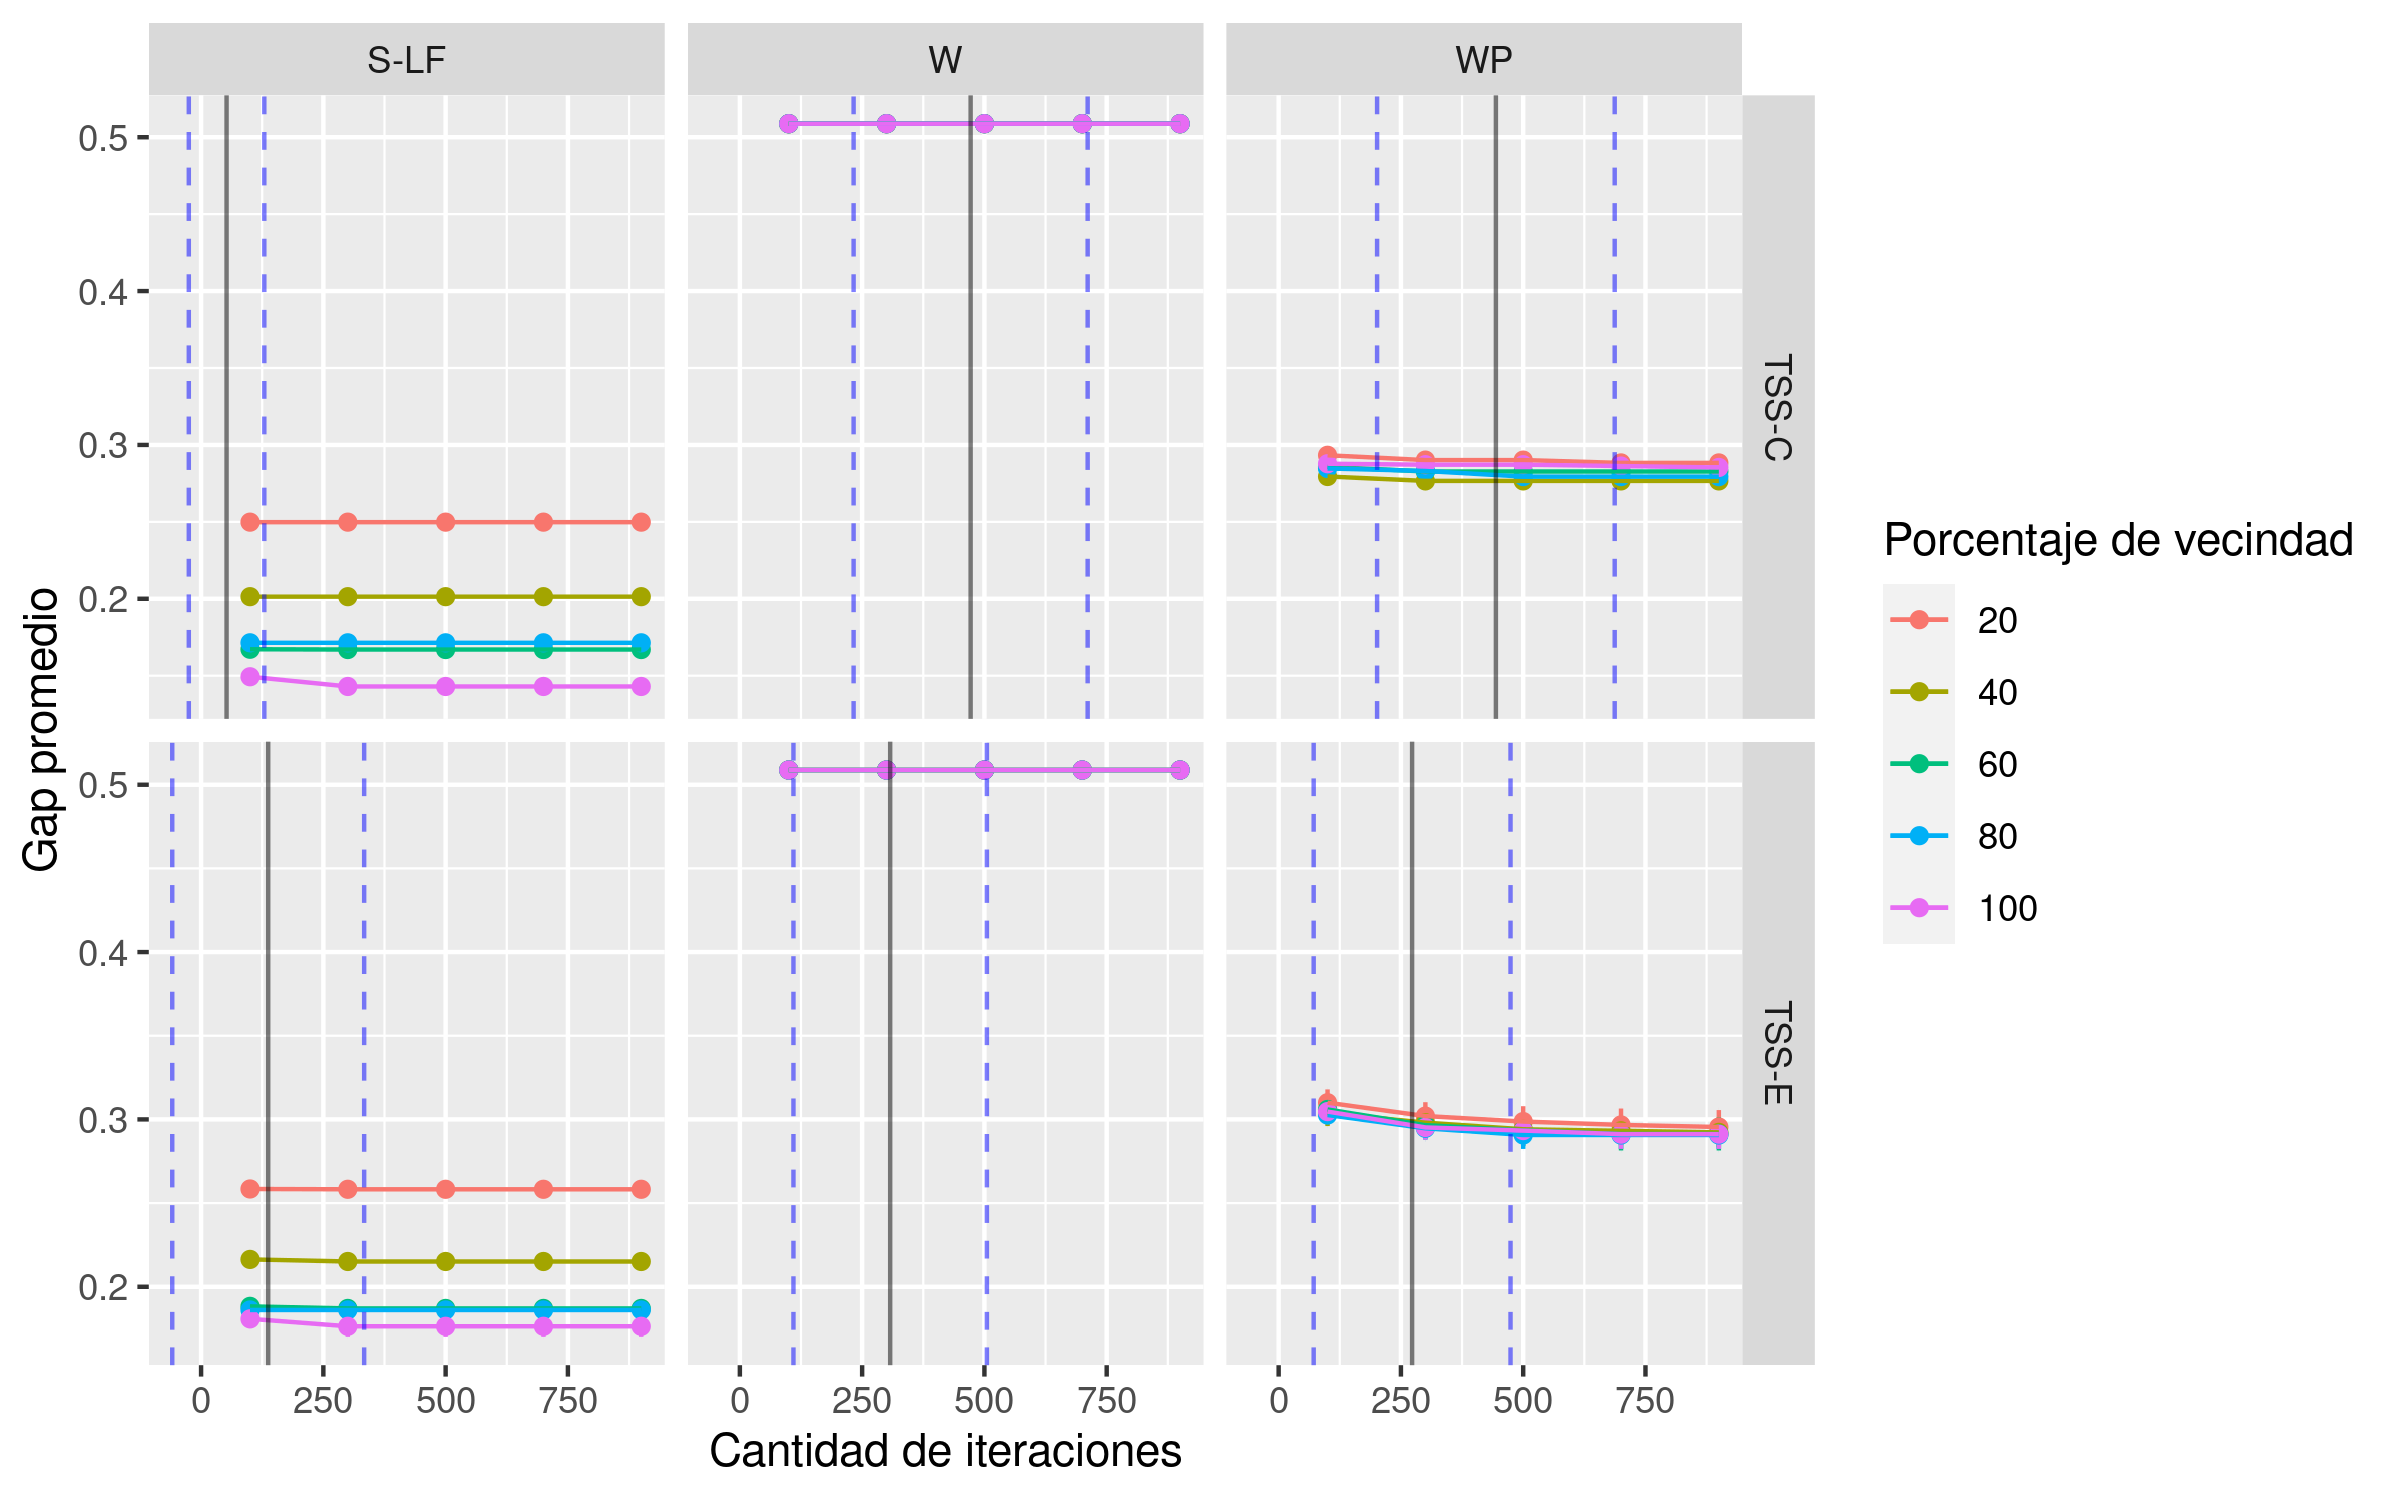
\includegraphics[width=0.8\textwidth]{plots/iteraciones_tss.png}
    \caption{Se observa el gap promedio en función de la cantidad de memoria para todas las combinaciones de tabú search swap y los algoritmos heurísticos iniciales. En todos los casos, se grafican los resultados obtenidos para valores de porcentaje de vecindad en [5, 20, 40, 60, 80, 100]. Se realizaron 5 repeticiones por instancia.}
    \label{plot:iteraciones tss}
\end{figure}

Considerando está sección y la anterior, ahora resulta más claro por qué había muchas combinaciones de parámetros que dan el mismo resultado en las Figura~\ref{plot:histogramas}. En general, se puede concluir que corridas con alta memoria o altas iteraciones terminan siendo equivalentes a las corridas que tienen valores cercanos a la cantidad de iteraciones efectivas.


\subsection{Evaluación}

Finalmente, para cada combinación de Tabú y heurística constructiva inicial, se eligieron las combinaciones que dieron mejor Gap en el set de datos de entrenamiento. En caso de que más de una configuración de parámetros diera resultados equivalentes se desempató por el tiempo de ejecución. Se detallan en la Tabla~\ref{tabla:ranking}.

En lineas generales no se observó correlación entre el tiempo de ejecución y la calidad de las soluciones entre los diferentes algoritmos de \textit{Tabú Search}. Esto puede observarse más en detalle en la fig. \ref{plot:correlacion gap tiempo}

Se puede observar que hay al menos un orden de magnitud de diferencia entre TSC usando heurística W o WP y el resto de los algoritmos, por lo que S-LF resulta la peor heurística constructiva para los TSC pero la mejor para los TSS por lo que explicado en la Sección 6.5. A su vez, notar que para TSC-E WP el número de iteraciones que da el mejor resultado es alto pero la diferencia en tiempo con las corridas que dan el resultado óptimo es muy chica, por lo que haber elegido ésta puede ser resultado de fluctuaciones experimentales. Sería interesante aumentar la cantidad de repeticiones y ver si se sigue eligiendo esta combinación de parámetros.

Por último, pareciera ser que la elección de estructura de Memoria no afecta el gap de TSS (salvo cuando usa S-LF porque tiene más posibilidades de encontrar mejorías), sólo el costo temporal. Aquí se confirma una vez más la importancia e injerencia del algoritmo inicial elegido en el desempeño del \textit{Tabú Swap}.

\begin{table}[ht]
\centering
\begin{tabular}{p{.5cm}p{1.5cm}p{1.8cm}p{1.8cm}p{2cm}p{1.8cm}p{1cm}p{1cm}p{1cm}}
  \hline
 & Variante de tabu & Heurística Inicial & Iteraciones & Porcentaje de Vecindad & Cantidad de Memoria & Aspirar & Gap medio & Tiempo medio (s) \\ 
  \hline
1 & TSC-C & WP & 300 & 90 & 100 & Si & 0 & 4.50 \\ 
  2 & TSC-E & W & 100 & 90 & 35 & Si & 0.003 & 1.04 \\ 
  3 & TSC-C & W & 300 & 50 & 50 & No & 0.003 & 3.35 \\ 
  4 & TSC-E & WP & 900 & 100 & 50 & Si & 0.009 & 0.80 \\ 
  5 & TSC-C & S-LF & 300 & 100 & 50 & Si & 0.089 & 2.68 \\ 
  6 & TSC-E & S-LF & 300 & 70 & 35 & Si & 0.131 & 0.34 \\ 
  7 & TSS-C & S-LF & 300 & 100 & 50 & No & 0.137 & 3.37 \\ 
  8 & TSS-E & S-LF & 300 & 100 & 100 & Si & 0.154 & 4.47 \\ 
  9 & TSS-E & WP & 500 & 60 & 100 & Si & 0.271 & 10.56 \\ 
  10 & TSS-C & WP & 700 & 25 & 35 & Si & 0.271 & 15.29 \\ 
  11 & TSS-E & W & 100 & 5 & 20 & No & 0.509 & 1.85 \\ 
  12 & TSS-C & W & 100 & 5 & 20 & Si & 0.509 & 2.20 \\ 
   \hline
\end{tabular}
\caption{Cuadro comparativo que presenta la mejor combinación de metaparámetros para cada algoritmo evaluado (combinación de tabú search y heurísticas iniciales). Se ordenan las entradas según el valor de gap promedio obtenido.}
\label{tabla:ranking}
\end{table}

Para analizar el desempeño de los algoritmos en instancias de testeo y evitar así cualquier tipo de \textit{overfitting} se corrió cada combinación de algoritmo tabú con inicial, utilizando los parámetros óptimos encontrados en el entrenamieinito. Los resultados se detallan en la Figura~\ref{plot:ranking}.

\begin{figure}[H]
    \centering
    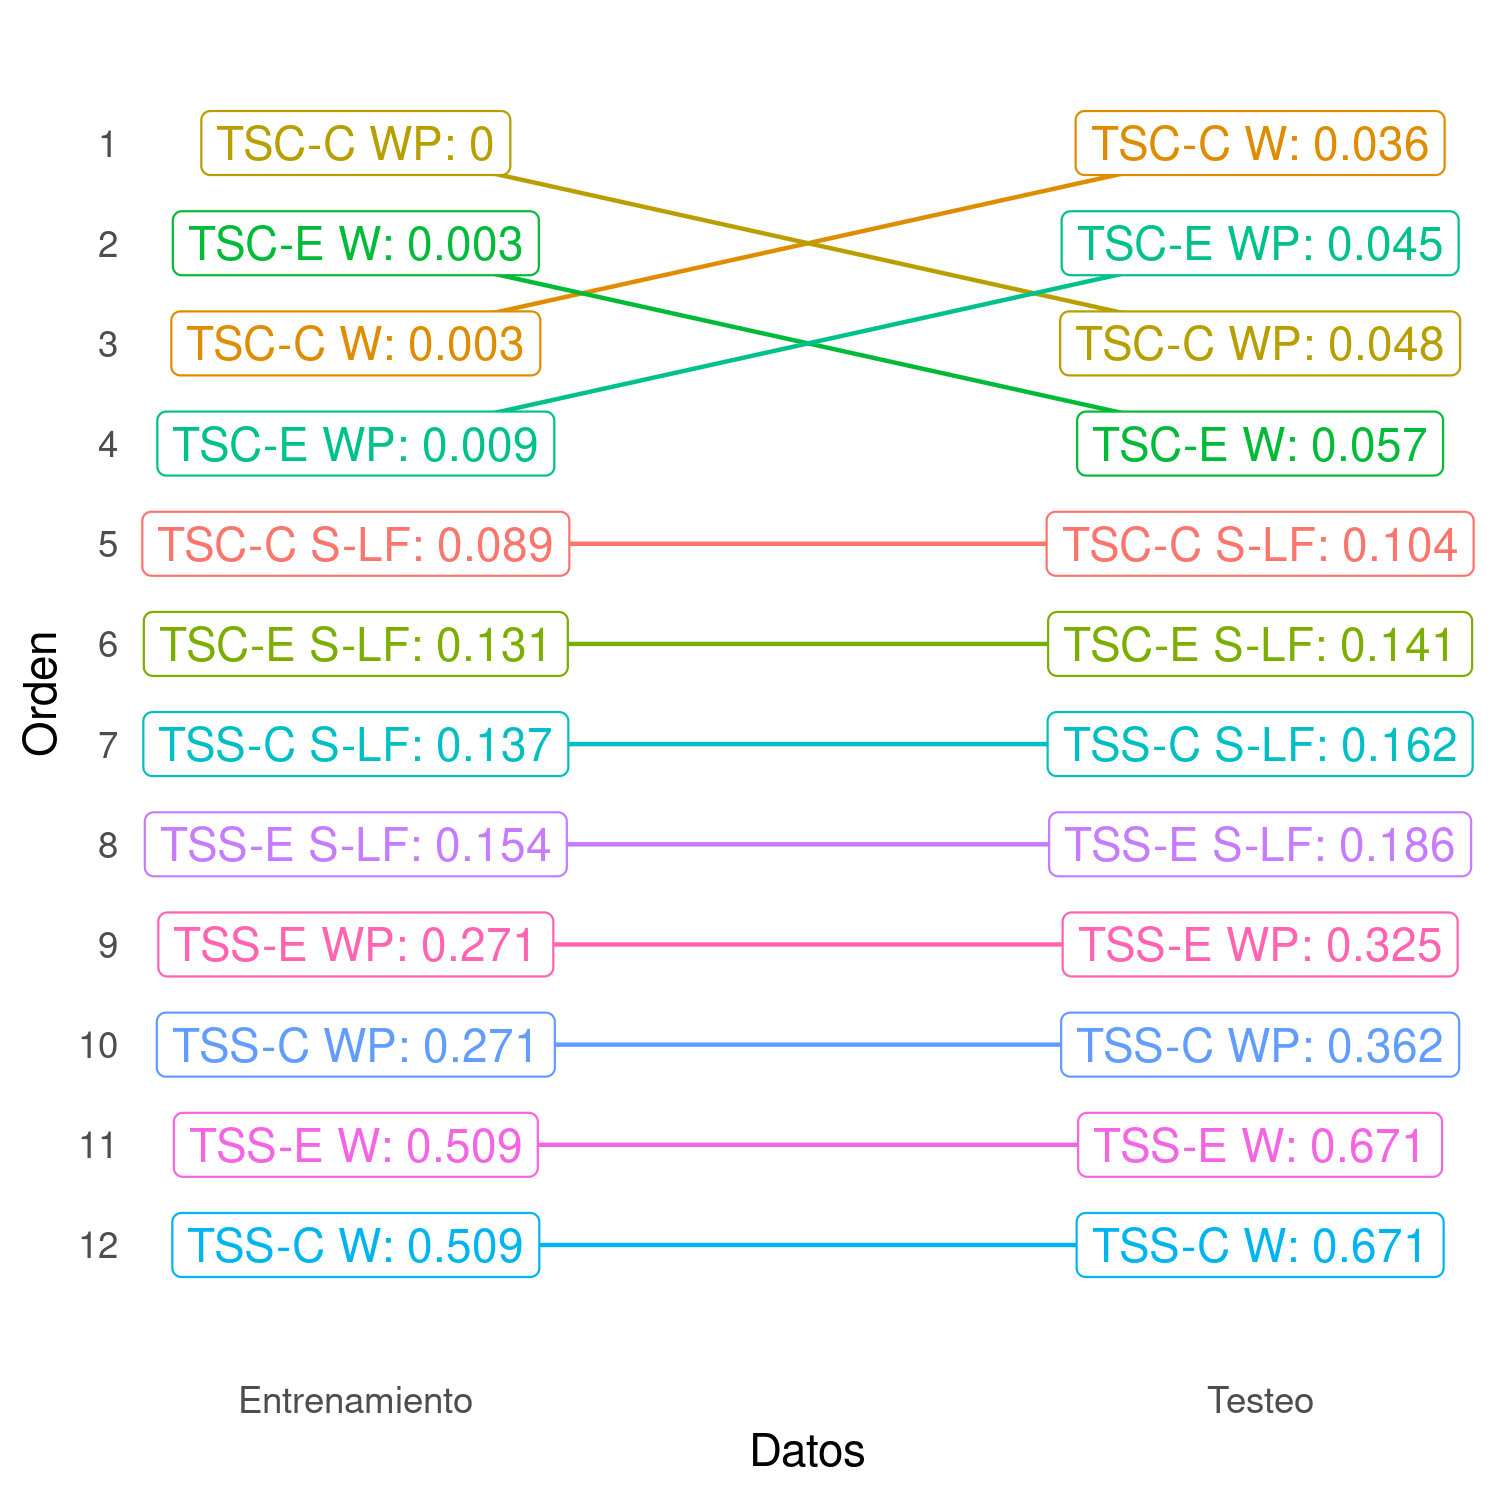
\includegraphics[scale = 0.7]{plots/ranking.png}
    \caption{Se observa el orden o ranking de algoritmos según los valores obtenidos de gap medio. A la izquierda se observa el ranking calculado para las instancias de entrenamiento, mientras que a la derecha, para las instancias de testeo.}
    \label{plot:ranking}
\end{figure}

Los resultados con el set de datos de testeo son peores, lo cual es esperable pero podría estar indicando \textit{overfitting} en el entrenamiento, sobre todo para TSC-C WP que da gap 0 en las instancias de entrenamiento. Sin embargo, se mantiene la diferencia de al menos un orden de magnitud entre TSC usando heurística W o WP y el resto de los algoritmos, por lo que el orden de eficiencia de los algoritmos se mantiene.

\section{Conclusiones}

En este trabajo se presentaron distintas técnicas para resolver PCMI, que resulta aplicable a problemas de la vida real. Se corrieron los algoritmos desarrollados para instancias de distintos tamaños, analizando y comparando el tiempo de ejecución y la calidad de las soluciones encontradas.

Se entrenaron los parámetros óptimos de Tabú Search (TS) en un subconjunto de instancias de \textit{train}, y se corroboraron en instancias de \textit{test} obteniendo buenos resultados.

Se pudo concluir que los algoritmos golosos son buenos para el costo computacional que implican, pero vale la pena invertir el tiempo extra por la calidad que brinda TS. Se probó que TS puede resolver el problema de forma satisfactoria cuando la generación de la vecindad emplea la estrategia de change. Cabe destacar que en este caso es importante emplear como heurística inicial a W o WP.

Sería interesante repetir la experimentación en un número de instancias mayor para poder determinar con mayor seguridad el ranking de las diferentes implementaciones de TSC que dieron un gap relativo muy similar.
\section{Apéndice}

\begin{figure}[H]
    \centering
    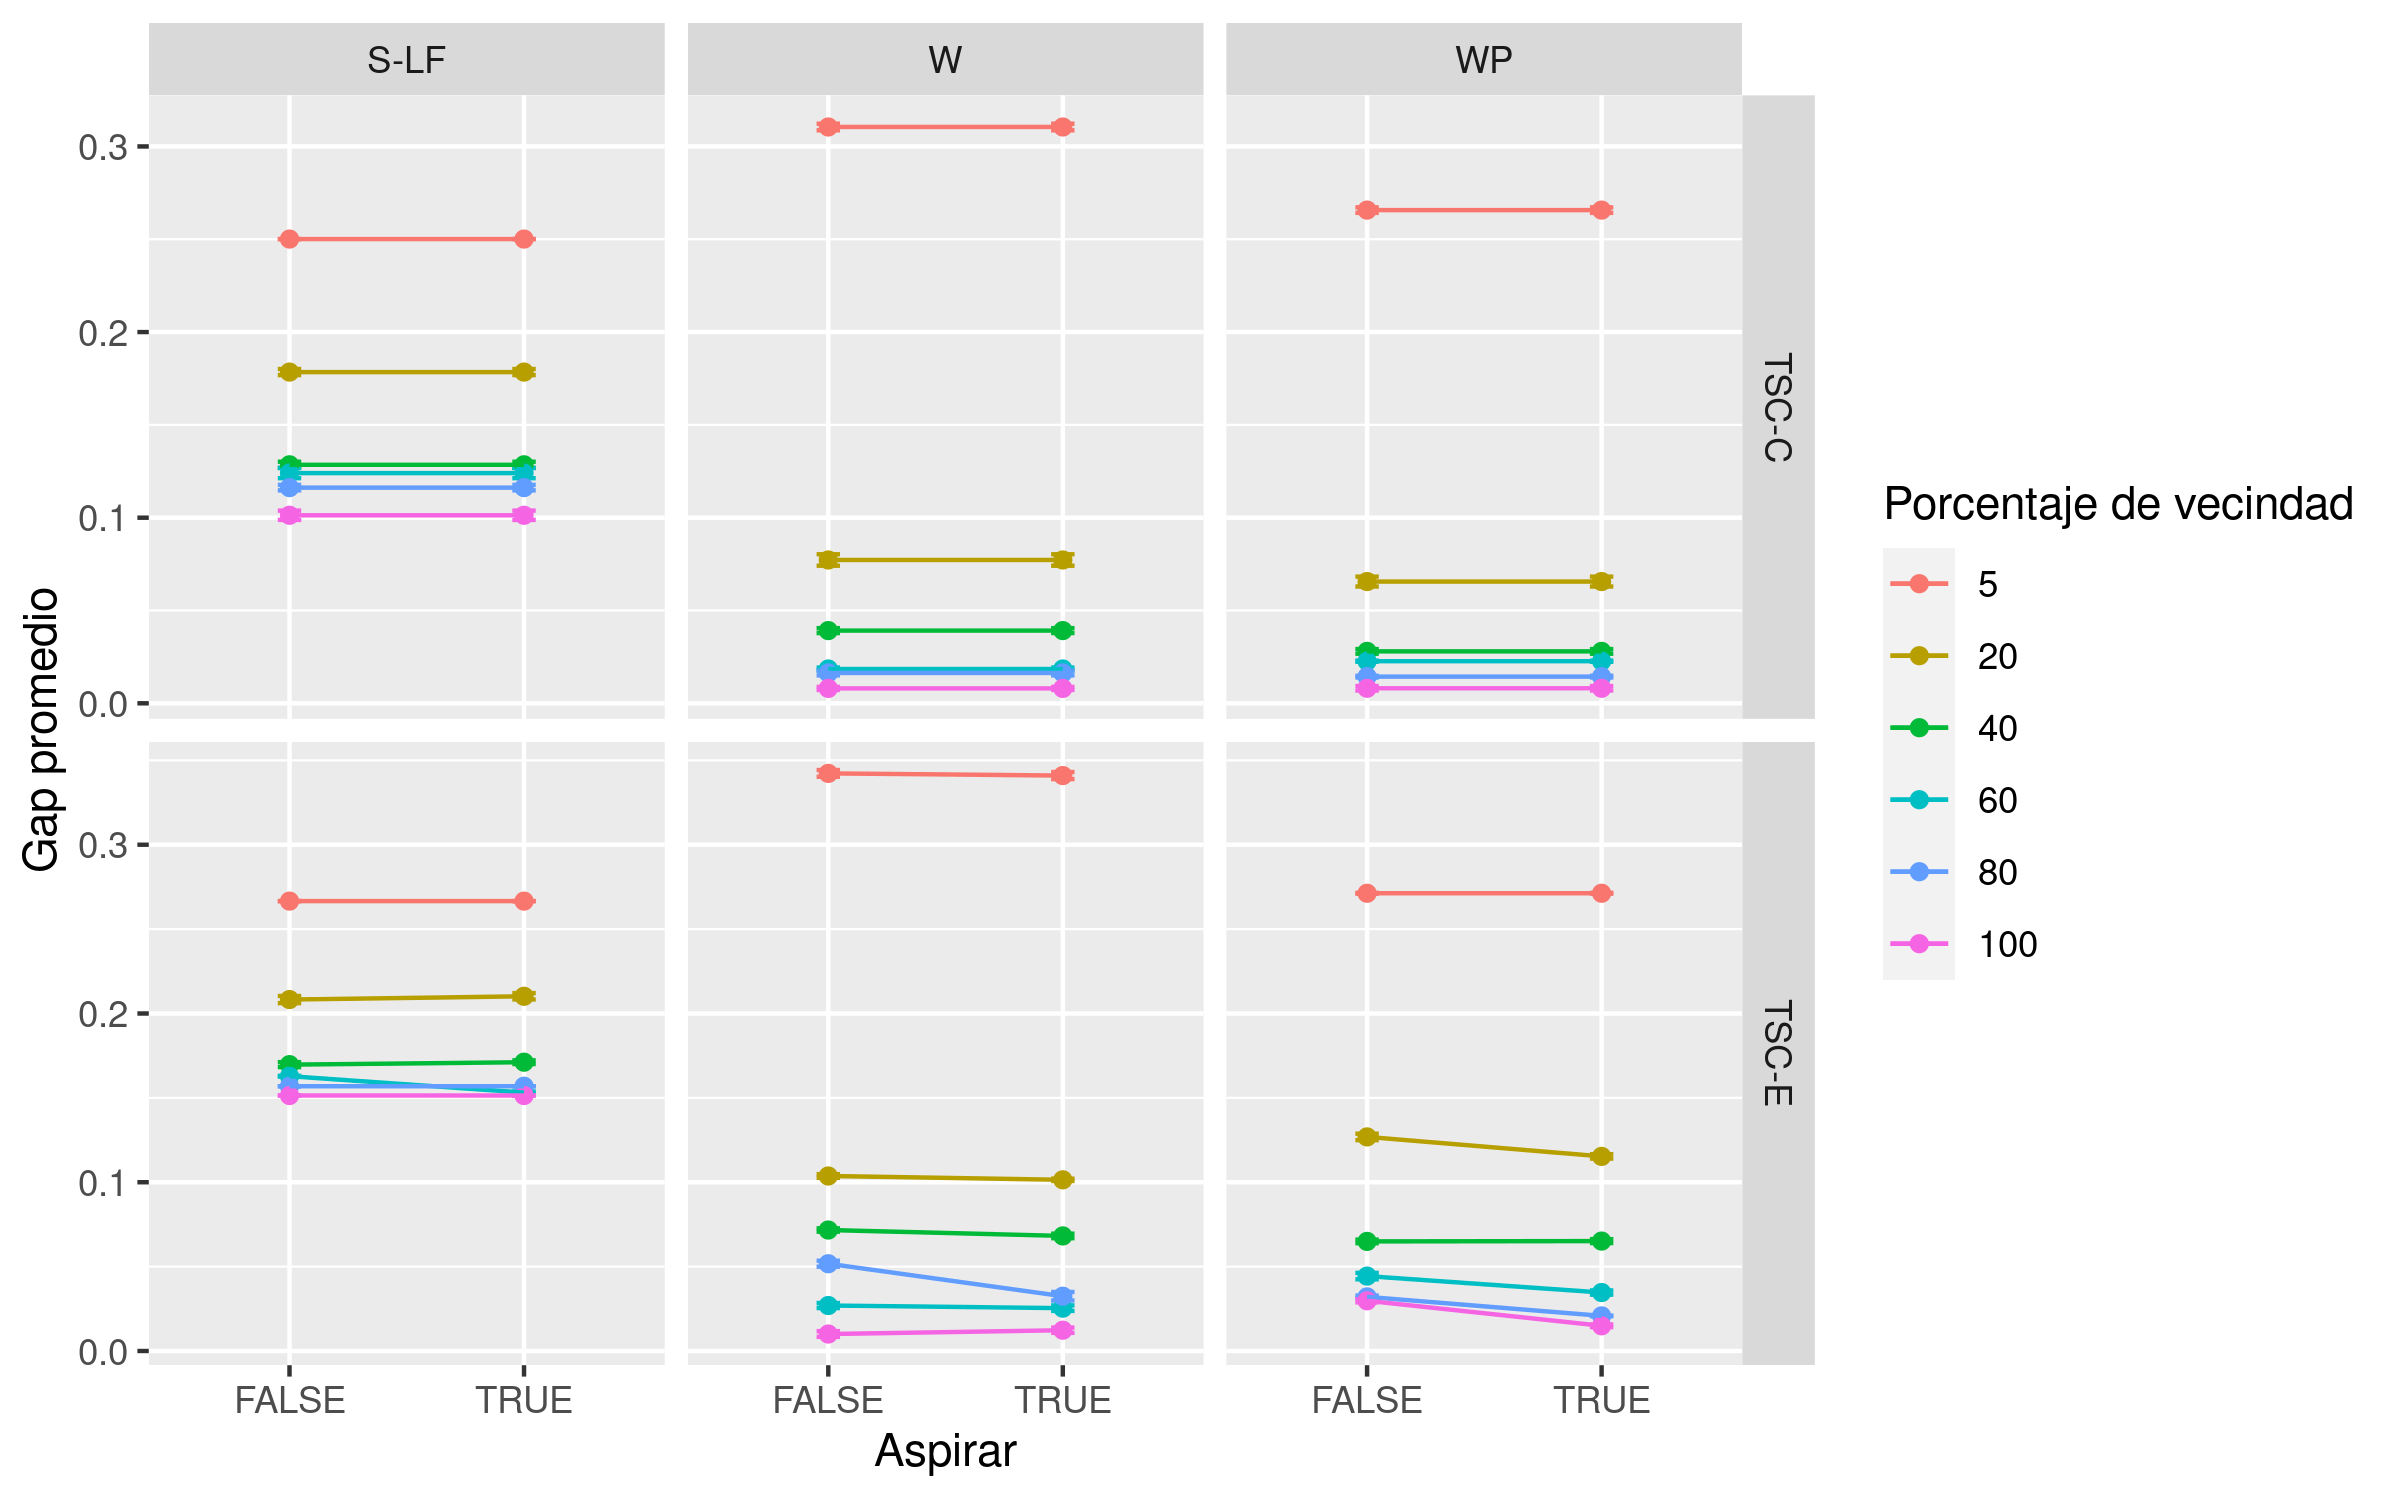
\includegraphics[scale = 0.7]{plots/suplementarias/aspirar_tsc.png}
    \caption{Gap relativo medio para ejecuciones de TSS activando o no la aspiración. Cada panel representa una combinación de heurística constructiva inicial y tipo de memoria. Los puntos representan el valor medio y las barras el error estándar. Se realizaron 5 repeticiones por instancia.}
    \label{plot:aspirar tsc}
\end{figure}

\begin{figure}[H]
    \centering
    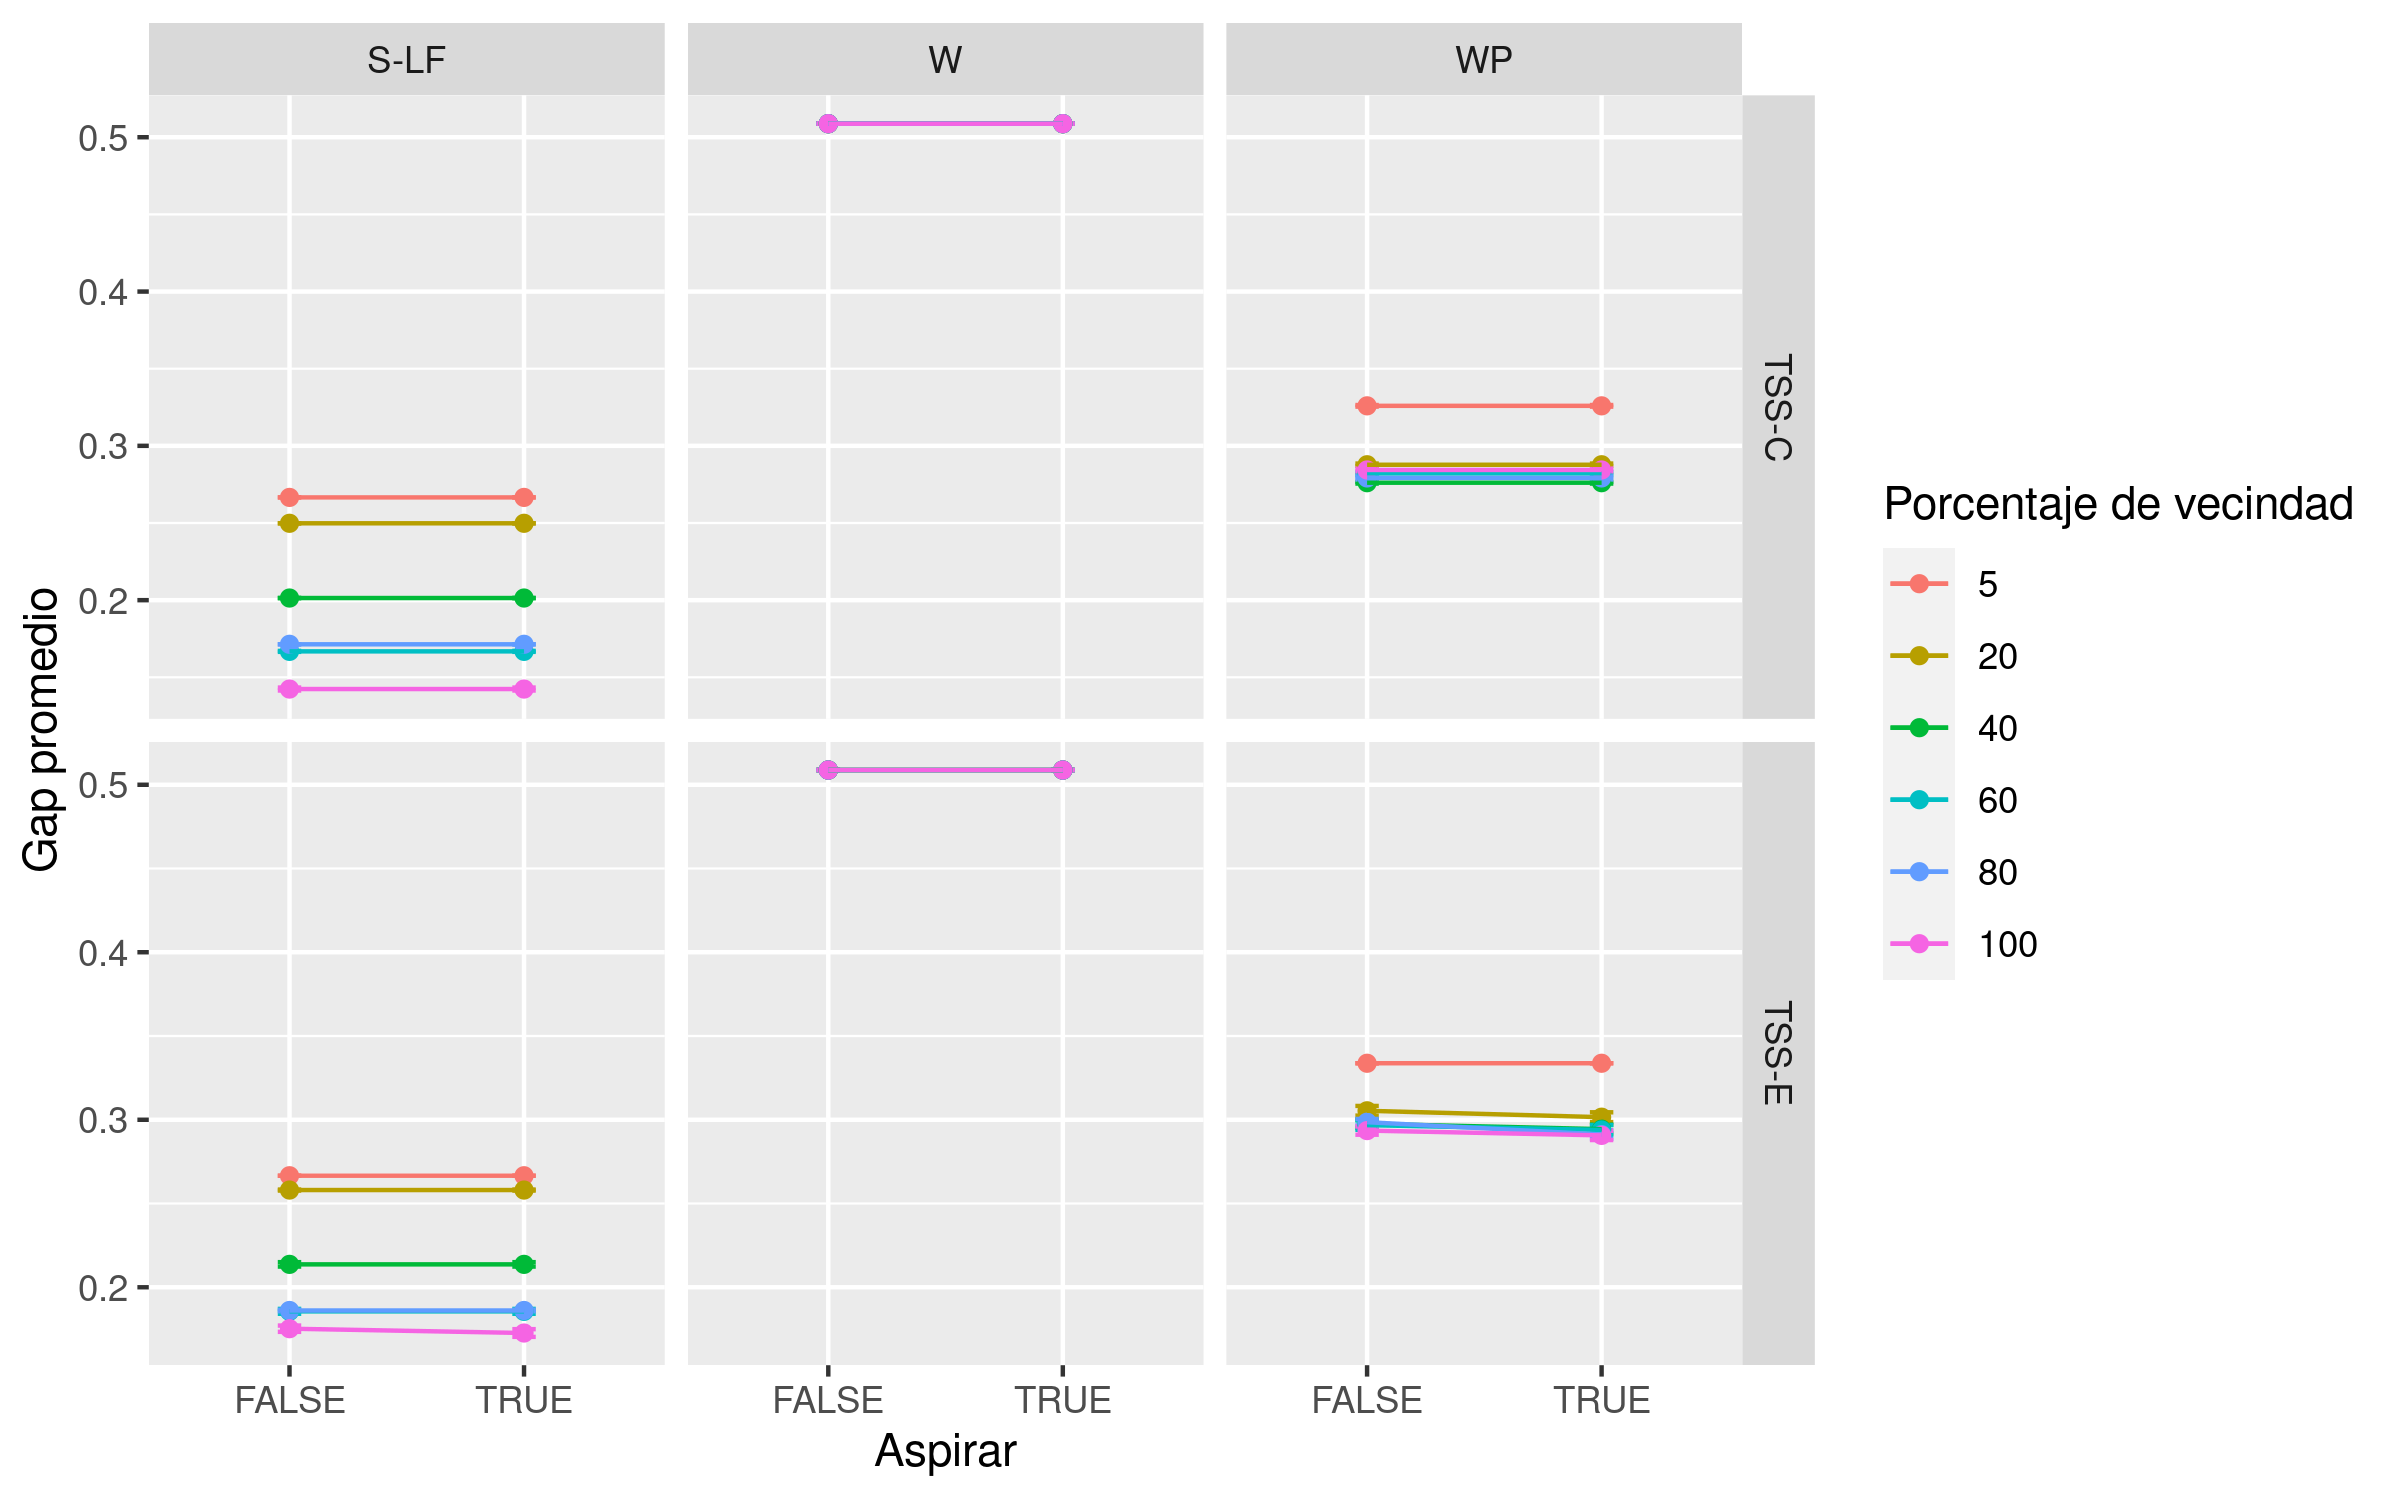
\includegraphics[scale = 0.7]{plots/suplementarias/aspirar_tss.png}
    \caption{Gap relativo medio para ejecuciones de TSS activando o no la aspiración. Cada panel representa una combinación de heurística constructiva inicial y tipo de memoria. Los puntos representan el valor medio y las barras el error estándar. Se realizaron 5 repeticiones por instancia.}
    \label{plot:aspirar tss}
\end{figure}


\begin{figure}[H]
    \centering
    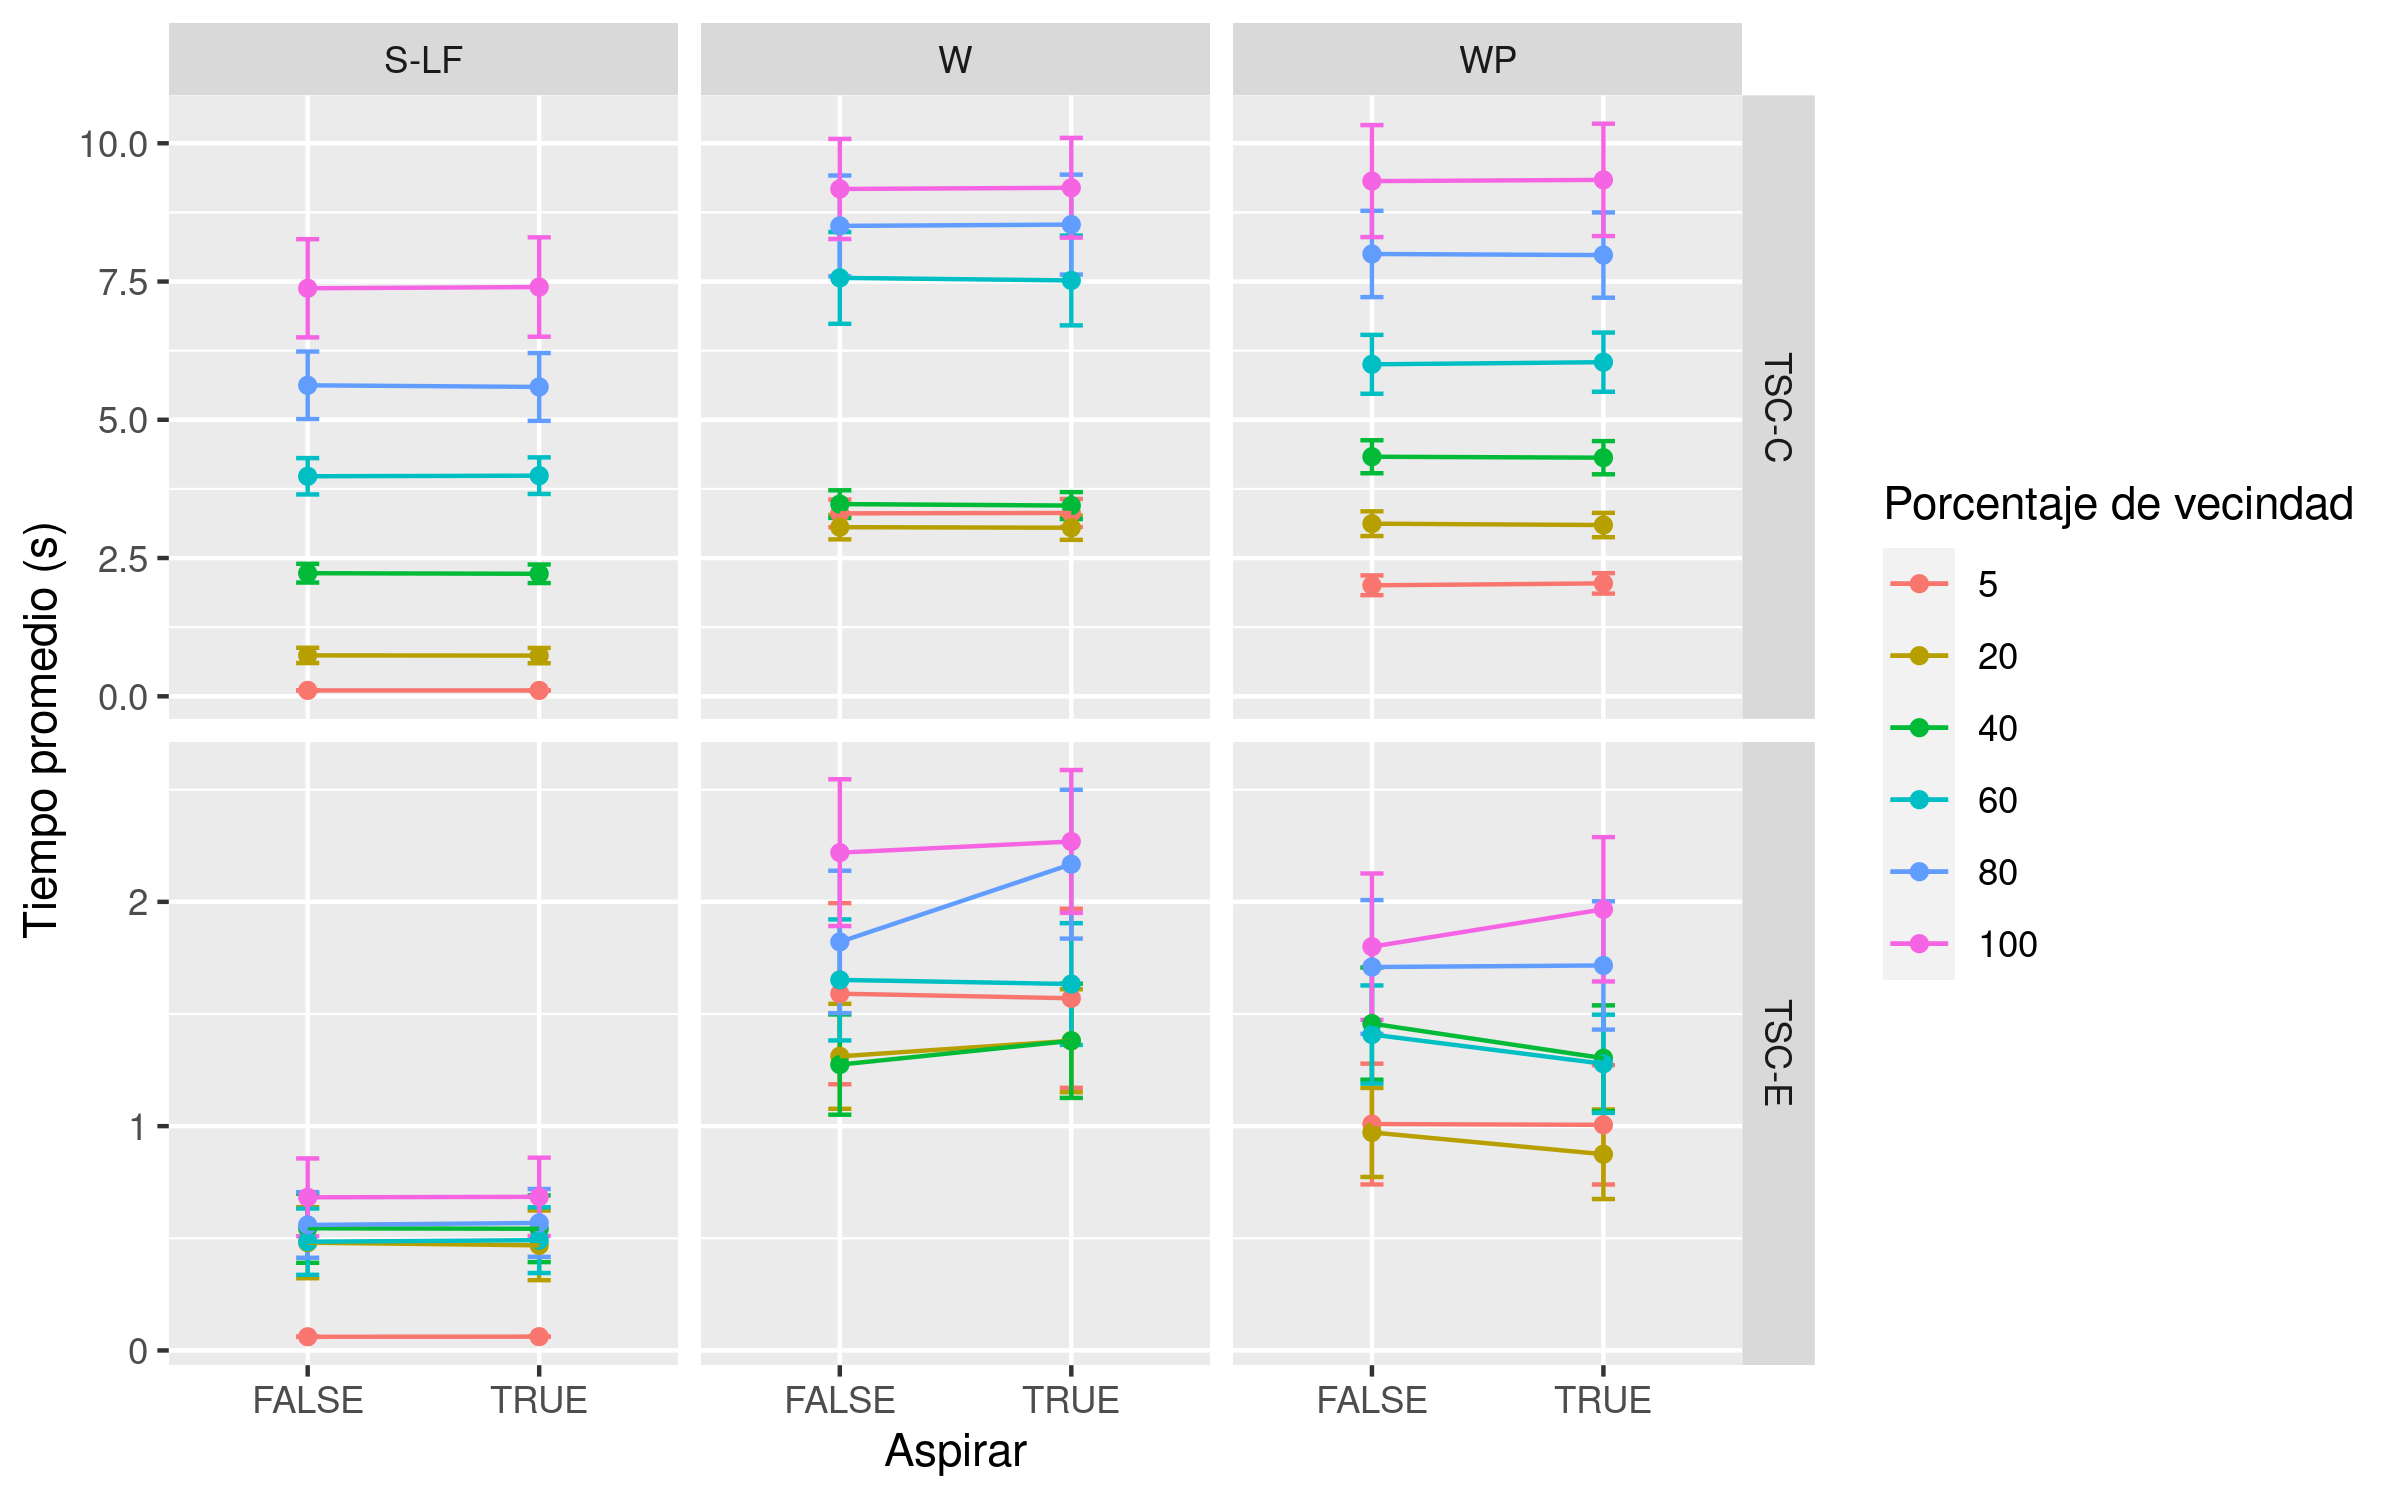
\includegraphics[scale = 0.7]{plots/suplementarias/aspirar_tiempo_tsc.png}
    \caption{Tiempo de ejecución medio para ejecuciones de TSC activando o no la aspiración. Cada panel representa una combinación de heurística constructiva inicial y tipo de memoria. Los puntos representan el valor medio y las barras el error estándar. Se realizaron 5 repeticiones por instancia.}
    \label{plot:aspirar tiempo tsc}
\end{figure}

\begin{figure}[H]
    \centering
    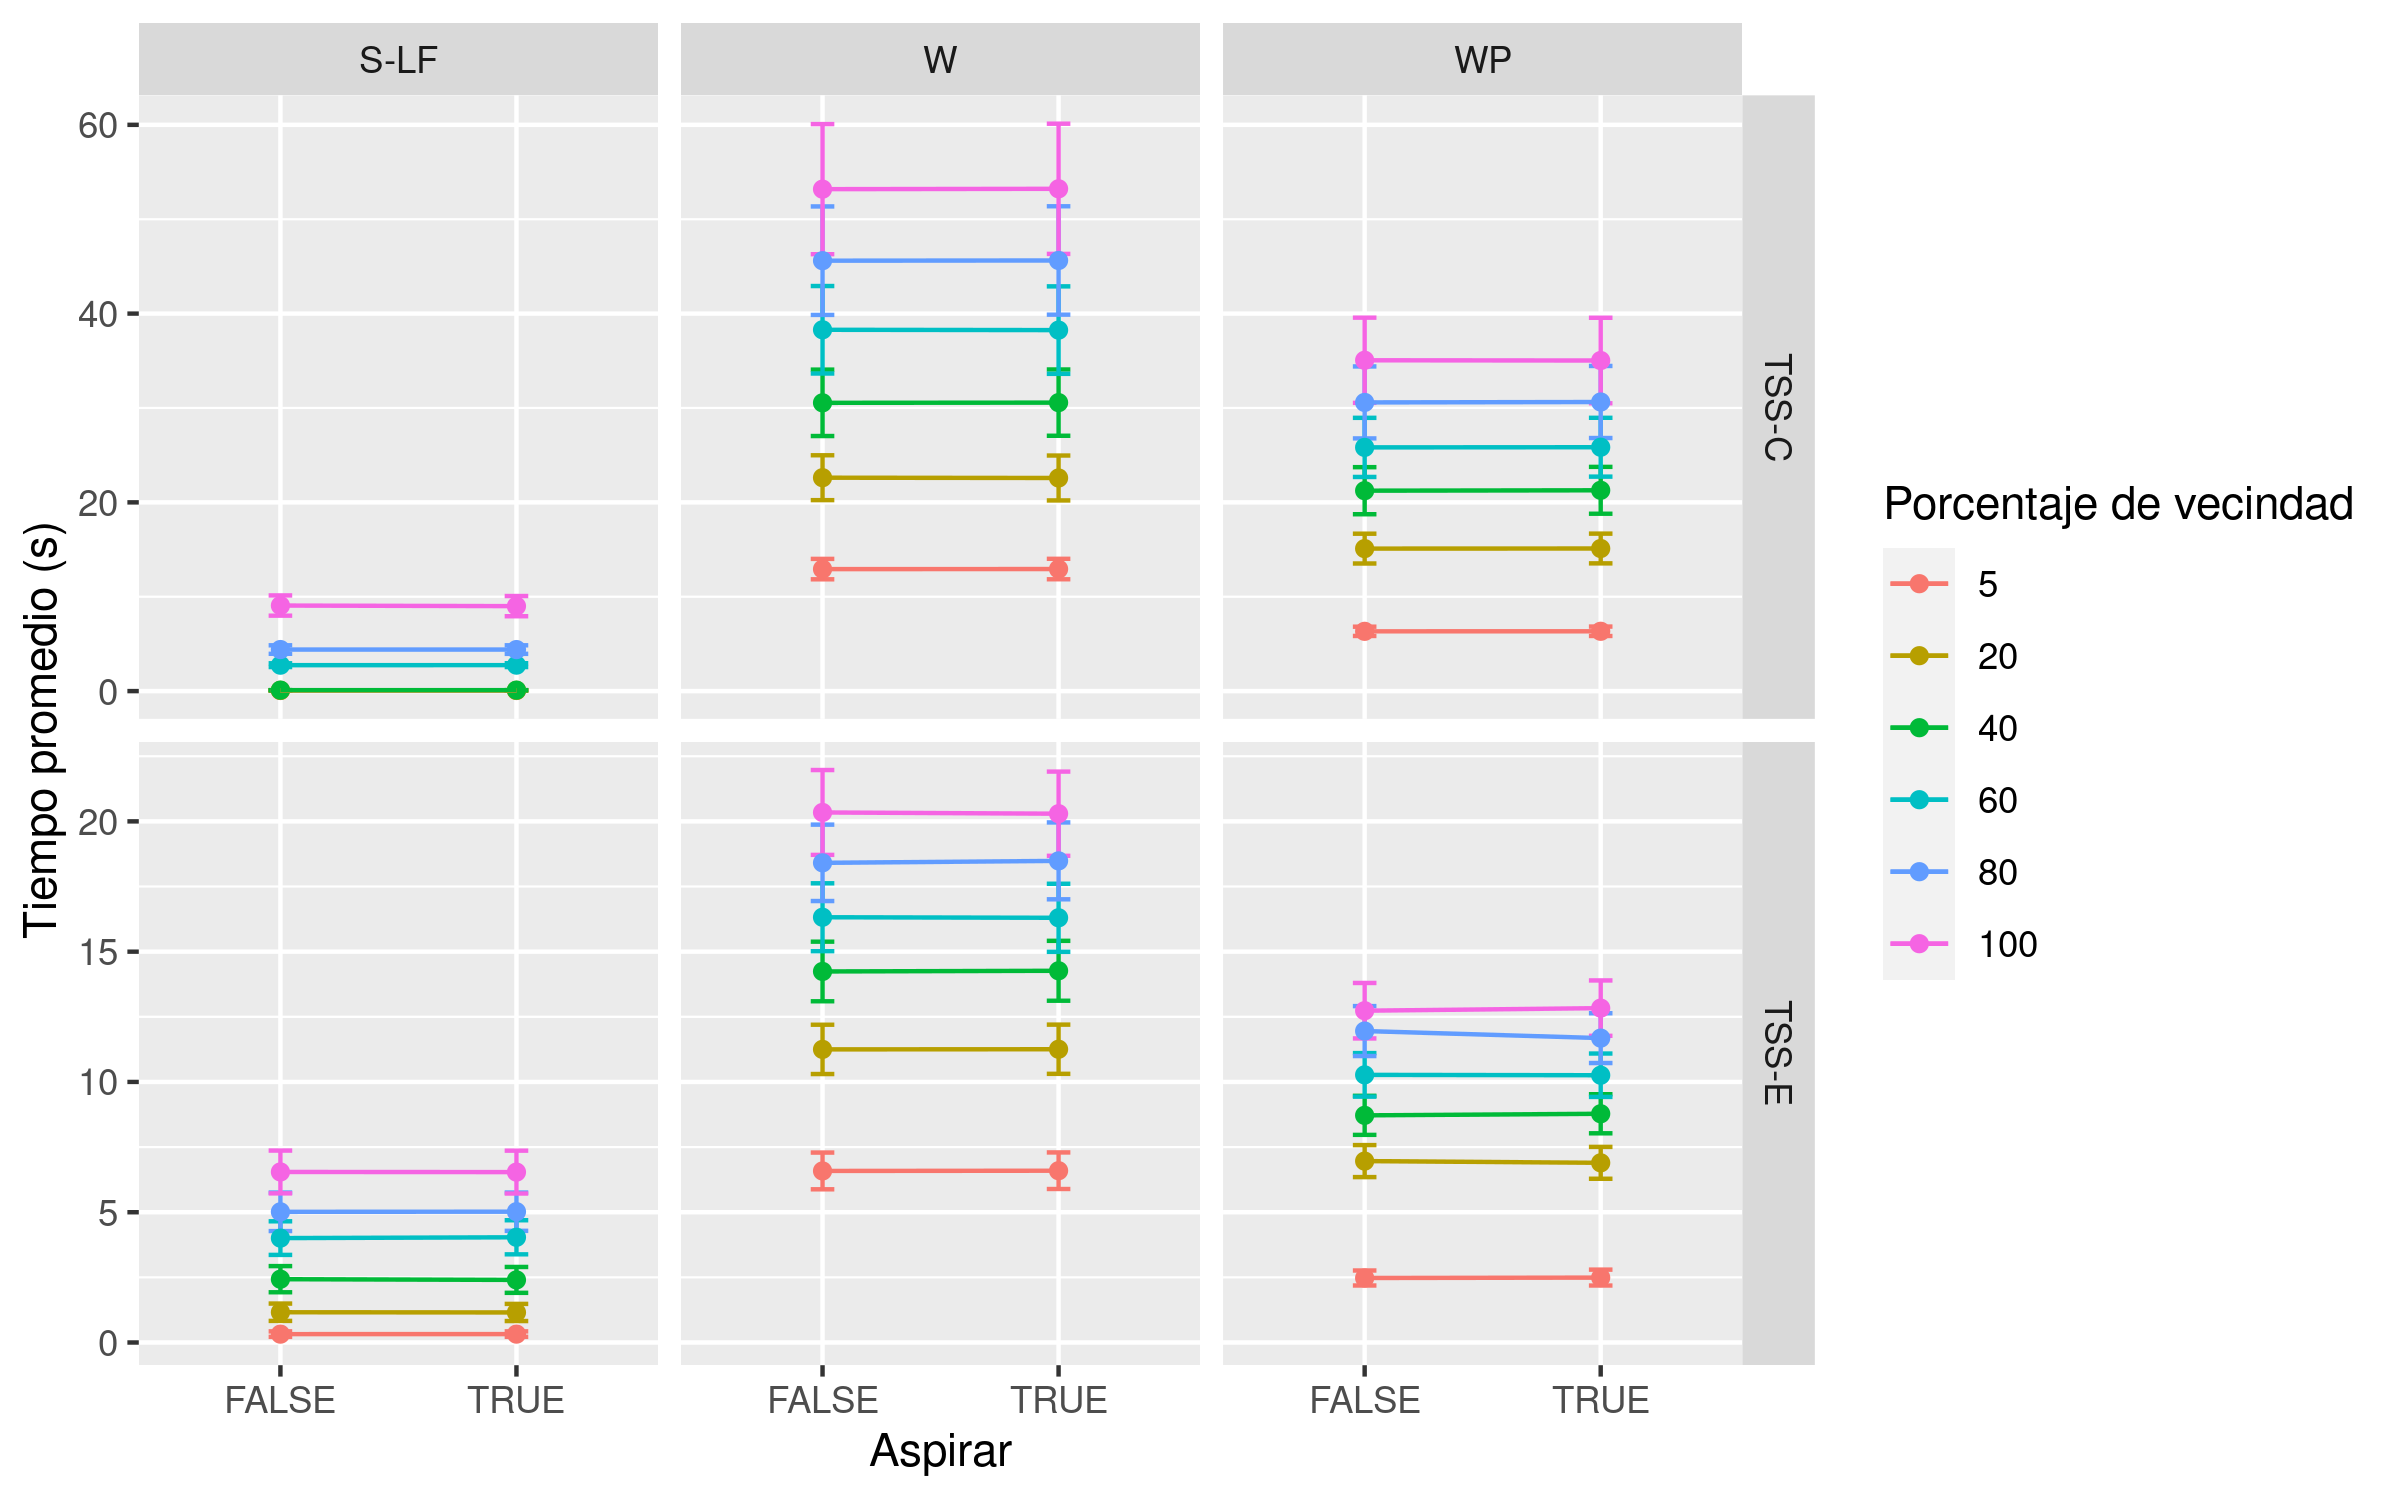
\includegraphics[scale = 0.7]{plots/suplementarias/aspirar_tiempo_tss.png}
    \caption{Tiempo de ejecución medio para ejecuciones de TSS activando o no la aspiración. Cada panel representa una combinación de heurística constructiva inicial y tipo de memoria. Los puntos representan el valor medio y las barras el error estándar. Se realizaron 5 repeticiones por instancia.}
    \label{plot:aspirar tiempo tss}
\end{figure}

\begin{figure}[H]
    \centering
    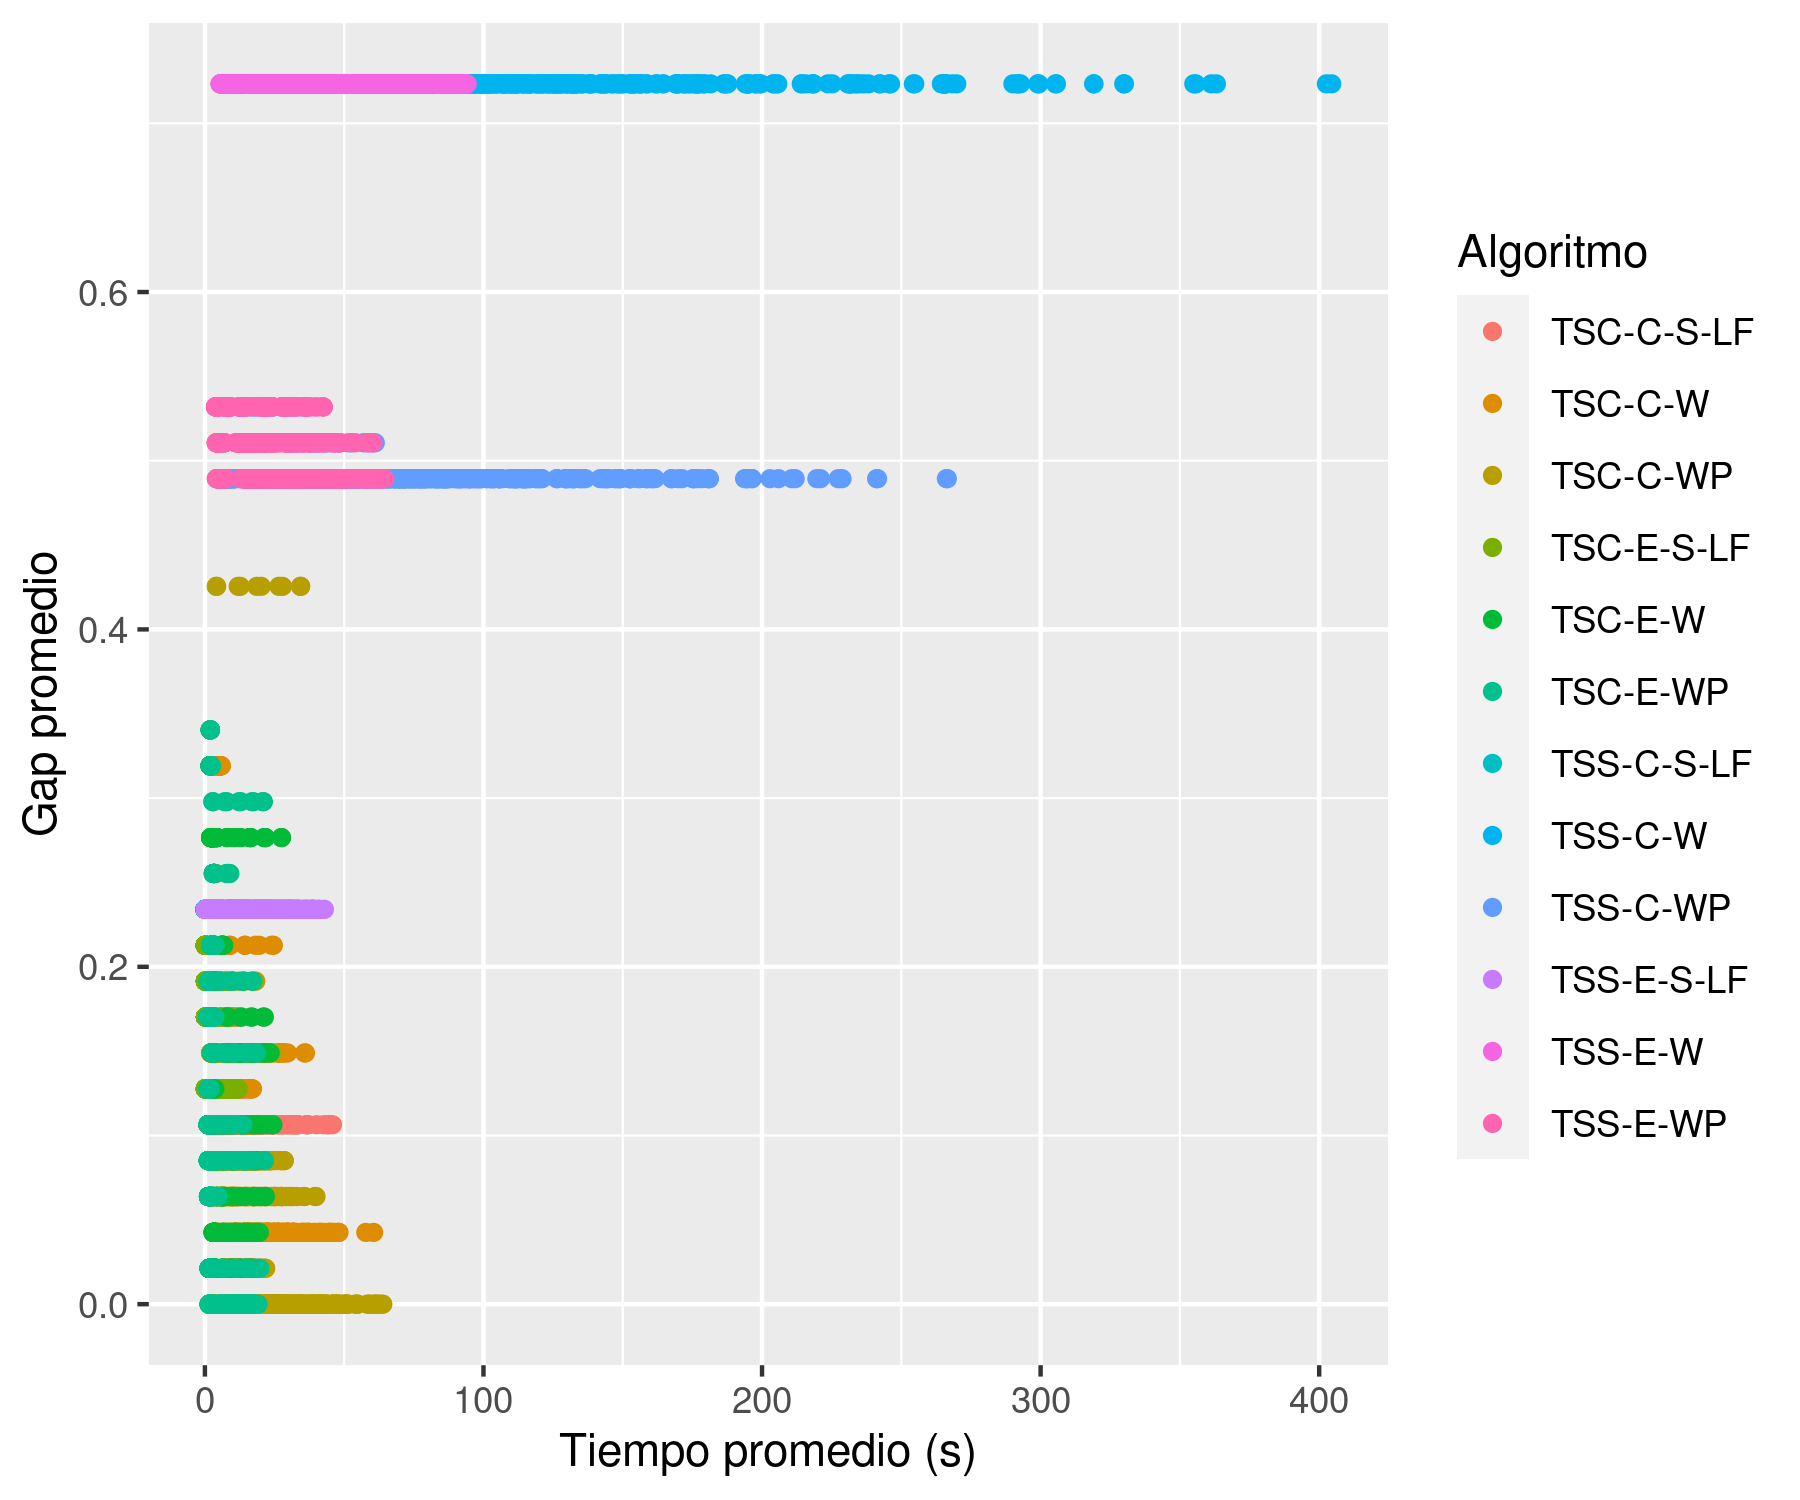
\includegraphics[scale = 0.7]{plots/suplementarias/gap_tiempo.png}
    \caption{Gap relativo promedio en función del tiempo promedio de ejecución. Los puntos representan el valor medio. Se realizaron 5 repeticiones por instancia. No se observa correlación.}
    \label{plot:correlacion gap tiempo}
\end{figure}

\end{document}